% Las imágenes ponerlas en la carpeta ./gfx

\documentclass[a4paper]{my_class}

\newcommand{\codigoMateria}{86.06}
\newcommand{\nombreMateria}{Circuitos Electrónicos}
\newcommand{\nroTP}{1}
\newcommand{\descripcionTP}{Amplificadores Operacionales: Usos y limitaciones}
\newcommand{\tituloTP}{Trabajo de Laboratorio N\grad \nroTP}
\newcommand{\facultad}{Facultad de Ingeniería}
\newcommand{\universidad}{Universidad de Buenos Aires}

\newcommand{\cuatri}{1er Cuatrimestre de 2015}

\usepackage{my_style}

% ---------------------------------------------------------------
% COMIENZO
\begin{document}
\nocite{*}
% ---------------------------------------------------------------
% TÍTULO Y PRESENTACIÓN
%******************************************************
%* Luciano Leonel Chamorro (FIUBA #95691)
%******************************************************
% Notas:
% Para cambiar el nombre de los integrantes, solo tocar los campos de "\teammember".
% El resto son comandos para compaginar la carátula
% -----------------------------------------------------

\thispagestyle{empty}
\newgeometry{twoside, left=2.5cm,top=2cm,right=2.5cm,bottom=1.5cm,bindingoffset=.5cm}
\begin{titlepage}

\begin{center}

\rule{\textwidth}{1.6pt}\vspace*{-\baselineskip}\vspace*{2pt}
\rule{\textwidth}{0.4pt}\\[.6\baselineskip]
{\LARGE
\textbf{\codigoMateria} \\[.6\baselineskip]
\nombreMateria} \\[.2\baselineskip]

\rule{\textwidth}{0.4pt}\\[.6\baselineskip]

{\Large
\tituloTP \\[.6\baselineskip]
\textbf{\descripcionTP} \\[.6\baselineskip]}

\rule{\textwidth}{0.4pt}\vspace*{-\baselineskip}\vspace{3.2pt}
\rule{\textwidth}{1.6pt}\\[\baselineskip]
\scshape

\vfill

\begin{figure}[H]
        \centering
        \begin{subfigure}[b]{0.4\textwidth}
        \noindent{
                
\includegraphics[width=.8\textwidth]{gfx/UBA.jpg}
        \hfill
        }
        \end{subfigure}
        \begin{subfigure}[b]{0.4\textwidth}
        \noindent{
        \hfill
                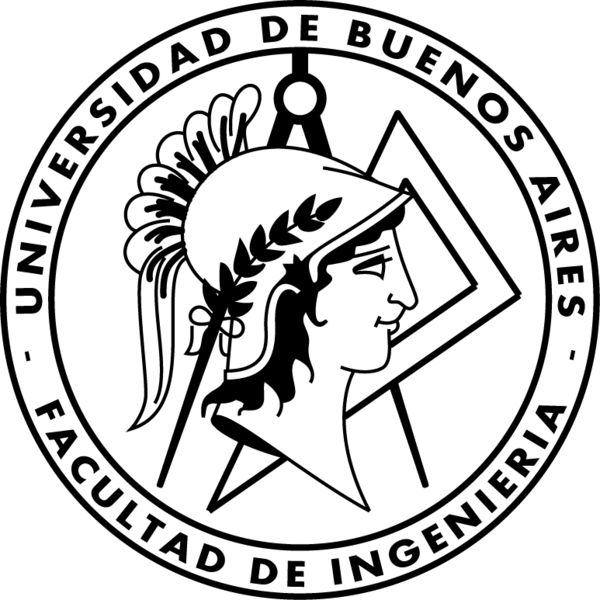
\includegraphics[width=.8\textwidth]{gfx/FIUBA.png}
        }
        \end{subfigure}
\end{figure}

%\vfill

\LARGE{\textsc{\underline{\universidad}}}\\[.6\baselineskip]
\Large{\textsc{\facultad}}\\[.6\baselineskip]
\large{\cuatri}

\end{center}

\vfill

\section*{Grupo de trabajo:}

\teammember
{Chamorro, Luciano L. \#95691}
{\href{mailto:luc.chamo@gmail.com}{$<$luc.chamo@gmail.com$>$}}

\teammember
{Corvalán, Hernán G. \#92780}
{\href{mailto:hgcorvala@gmail.com}{$<$hgcorvala@gmail.com$>$}}

\teammember
{Román, Santiago \#93947}
{\href{mailto:santiago_roman@outlook.com}{$<$santiago\_roman@outlook.com$>$}}


\section*{Docentes:}

\teammember
{Zola, Julio G.}
{}{}


\teammember
{Kelly, Juan M.}
{}{}

\teammember
{Ferro, Oscar R.}
{}{}




\vfill

\vspace{1cm}
\hrule
\vspace{0.2cm}

\noindent\small{\today \hfill Ciudad Autónoma de Buenos Aires, Argentina}

\end{titlepage}
\restoregeometry 
\thispagestyle{empty}
\cleardoublepage

\pagenumbering{Roman}

% ABSTRACT
%\include{S0}
%\thispagestyle{empty}
%\cleardoublepage

% TABLA DE CONTENIDOS
\tableofcontents 
\cleardoublepage
% ---------------------------------------------------------------
% PARTE PRINCIPAL
\pagenumbering{arabic}
\pagestyle{fancy}

\section{Introducción}
\label{sec:intro}


El presente trabajo se basa en el estudio de diversos tipos de circuitos que se pueden lograr utilizando amplificadores operacionales, buscando entender su funcionamiento, comportamiento ideal y, tras haber realizado las correspondientes mediciones en el laboratorio, concluir respecto de cuales son las limitaciones de ese modelo. Además, se analizan dos tipos de circuitos rectificadores de media onda, estudiando cómo varía su funcionamiento al modificar la carga, aumentar la frecuencia, entre otros.

{\bf El barrido en frecuencia de la figura 2.14 creo que convendría hacerlo en dB y el eje de la frecuencia logarítmico. De esa manera va a ser más fácil identificar el polo.}

\todo[inline, color=green!40]{Listo ahi lo arregle - Santiago.}

{\bf Che, estoy pensando en cómo justificar la respuesta del filtro logarítmico... y la verdad, no los entiendo del todo los gráficos de Vo/vi... son las señales que parten de las imágenes 39, 40 y 41. Si les llega a agarrar algo de interés, podrían chequearlo? - Osea, el gráfico hay que verlo al revés porque invierte, y se le ve "un poco la forma del logaritmo", pero no estoy seguro de eso...}

\todo[inline, color=green!40]{No se si cambiaste algo desde que hiciste este comentario pero no hay imágenes 39,40 y 41 jaja. Respecto de las figuras que hacen Vo vs Vi lo acabo de ver y tampoco lo entiendo, si se me ocurre algo aviso. - Santiago.

jaja, me estaba refiriendo a las imagenes que sacamos del osciloscopio SCD0000039,40,41. ahí escribí algo... pero creo que es chamuyo..}

\todo[inline, color=red!40]{che, hay algo de la Fig. \ref{fig:multipl_a_idealvsmed} que no me cierra.
Contra qué están comparando el desfasaje? Contra la señal de entrada? Yo no veo que la fig 2.5 esté desfasada.
%Porque lo que entiendo yo de ese punto es que el desfasaje no lo provocaría el AO, sino que la carga capacitiva del osciloscopio.
Y en la fig 2.6, no es que hay desfasaje, están a distinta frecuencia nomás. La medida está a una frecuencia apenas un poco menor a 1kHz - No quiero tocar por si me equivoco, pero fíjense en eso. - Lucho}


\todo[inline, color=red!40]{En la pregunta de "aumentar a más de 0.4V y ver qué pasa" de la parte del inversor no me acuerdo qué pasaba. Recortaba la señal? atenuaba? Podrás extender un toque la respuesta?}



\todo[inline, color=red!40]{En la caption de las figuras de barrido de frecuencia del inversor, convendría poner si es de las mediciones o de simulación. cómo es? la primera es simulación x10 y la segunda es medición x1? (figuras 2.15 y 2.17}


\todo[inline, color=red!40]{Entonces... hay que hacer la medición de corriente para el rectificador agregándole una resistencia pequeña

corregir lo que decís del gráfico de esas "senoidales desfasadas"

corregir la respuesta a la última pregunta del inversor, (agregar una foto del análisis de fourier quizás), y explicar el fenómeno de la deformación de la senoidal al transformarla en triangular.}

\todo[inline, color=green!40]{Ahi puse lo del método para medir corriente que circula por el diodo, por si acaso que alguno le pegue una leída.

También corregí lo de las figuras de barrido en frecuencia que no aclaraban que correspondían a una simulación}



\clearpage
\section{Amplificadores}
\label{sec:ampli}

\subsection{Multiplicador por una constante}

%Breve Reseña
Aquí se analiza el amplificador operacional $(AO)$ como un amplificador de tensión o multiplicador por una constante. Para esto, se dispone de la siguiente configuración circuital:


\begin{figure}[h]
  \centering
      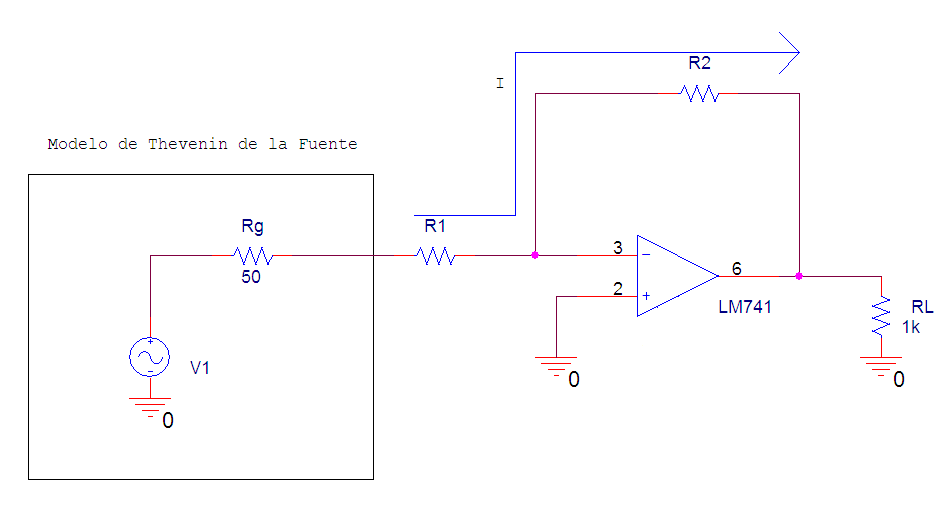
\includegraphics[width=0.7\textwidth]{gfxhernan/FIG21modif.PNG}
  \caption{Amplificador de Tensión o multiplicador por una constante}
  \label{circ:multipl}
\end{figure}
        
Para los cálculos se supondrá que el AO es ideal, de esta forma será sencillo obtener las corrientes y caídas de tensión en el circuito. Se calculan los valores de $v_{o}$ para distintos valores de $R_{1}$ y $R_{2}$. El valor de $R_{L}$, correspondiente a la carga, se mantiene fijo. Se comparan estos resultados con los obtenidos por una simulación en Spice que utiliza un modelo del LM741 otorgado por la cátedra y con los datos obtenidos a partir de las mediciones realizadas en el laboratorio.\\

\subsubsection{Señal de Salida con Amplificador Operacional como ideal}
Se parte del circuito de la figura \ref{circ:multipl}, donde la tensión de entrada es $ v_{i1}=\hat{V}_{1l} sen(wt)$, tal que $\hat{V}_{1l} = 0,2 V$ y la frecuencia es 1 $kHz$.

Para obtener el valor de $v_{o}$, se supone un AO ideal, es decir:
\begin{itemize}
\item la diferencia de tensión entre sus terminales de entrada es cero,
\item no circula corriente por los terminales de entrada,
\item la diferencia de tensión entre ambos nodos es 0 V,
\item la ganancia de tensión es infinita,
\item la impedancia de salida es infinito,
\item el operacional tiene una respuesta en frecuencia constante.
\end{itemize}
En la entrada hay una señal de valor pico 0,2 V y el terminal inversor se comporta como tierra virtual, por lo que se puede calcular la corriente que circula por $R_{1}$ :

$$i_{R1} = \frac{\hat{V}_{1l}.sen(wt)}{R_{1}}$$

El valor pico de la corriente es:

$$\hat{I}_{R1} = \frac{\hat{V}_{1l}}{R_{1}}$$

Por los terminales de entrada del operacional no circula corriente, la corriente $i_{R_{1}}$ circulará por $R_{2}$, provocando que en la carga caiga una tensión pico de:

$$ v_{o}=-i_{R1}R_{2}$$

La ganancia $Av = \frac{v_{o}}{v_{i}}$ resulta en $Av = \frac{-R_{2}}{R_{1}}$.

Al reemplazar por los valores de las siguientes resistencias:\\

\begin{center}
a) $R_{1}= 1k\Omega$ y $R_{2}=10 k\Omega$\\
b) $R_{1}= 1M\Omega$ y $R_{2}=10 M\Omega$\\
c) $R_{1}= 1k\Omega$ y $R_{2}=1 M\Omega$\\
\end{center}

De esta manera, se deberían obtener teórica e idealmente los siguientes valores de $v_{o}$:
\begin{center}
a) $v_{o} = -2Vsen(wt)$\\
b) $v_{o} = -2Vsen(wt)$\\
c) $v_{o} = -200Vsen(wt)$\\
\end{center}


\subsubsection{Simulación mediante Spice y Mediciones}
A continuación, se simula el circuito de la figura \ref{circ:multipl} mediante Spice. Se hace uso de un modelo del LM741, que luego se utilizará en las mediciones de laboratorio.

Se debe tener en cuenta que al medir la señal de salida haciendo uso del osciloscopio y las puntas de prueba directa (1x), se están agregando impedancias provenientes de los instrumentos. Es por ello que se puede modelar al osciloscopio y su correspondiente punta a través de un circuito equivalente, como el que se presenta en la siguiente figura \ref{circ:multipl_punta1x}:\\\\

\begin{figure}[h]
  \centering
      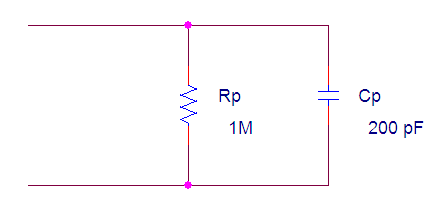
\includegraphics[width=0.5\textwidth]{gfx/fig2.png}
  \caption{Circuito equivalente del osciloscopio junto a la punta 1x}
  \label{circ:multipl_punta1x}
\end{figure}        


\begin{figure}[H]
  \centering
      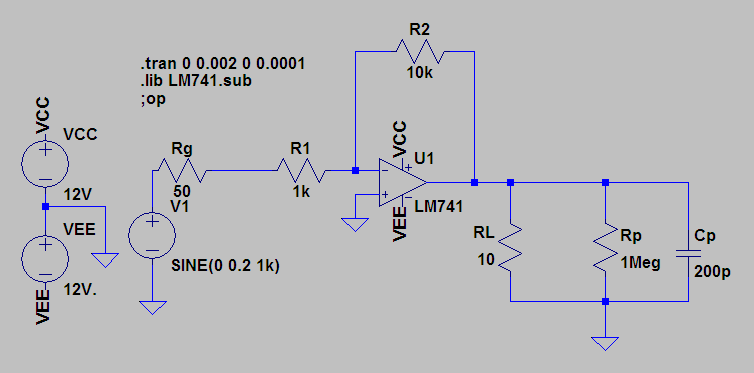
\includegraphics[width=0.7\textwidth]{gfxhernan/fig23.PNG}
  \caption{Banco de simulación en Spice}
  \label{circ:multipl_banco_sim}
\end{figure}        

\begin{figure}[H]
  \centering
      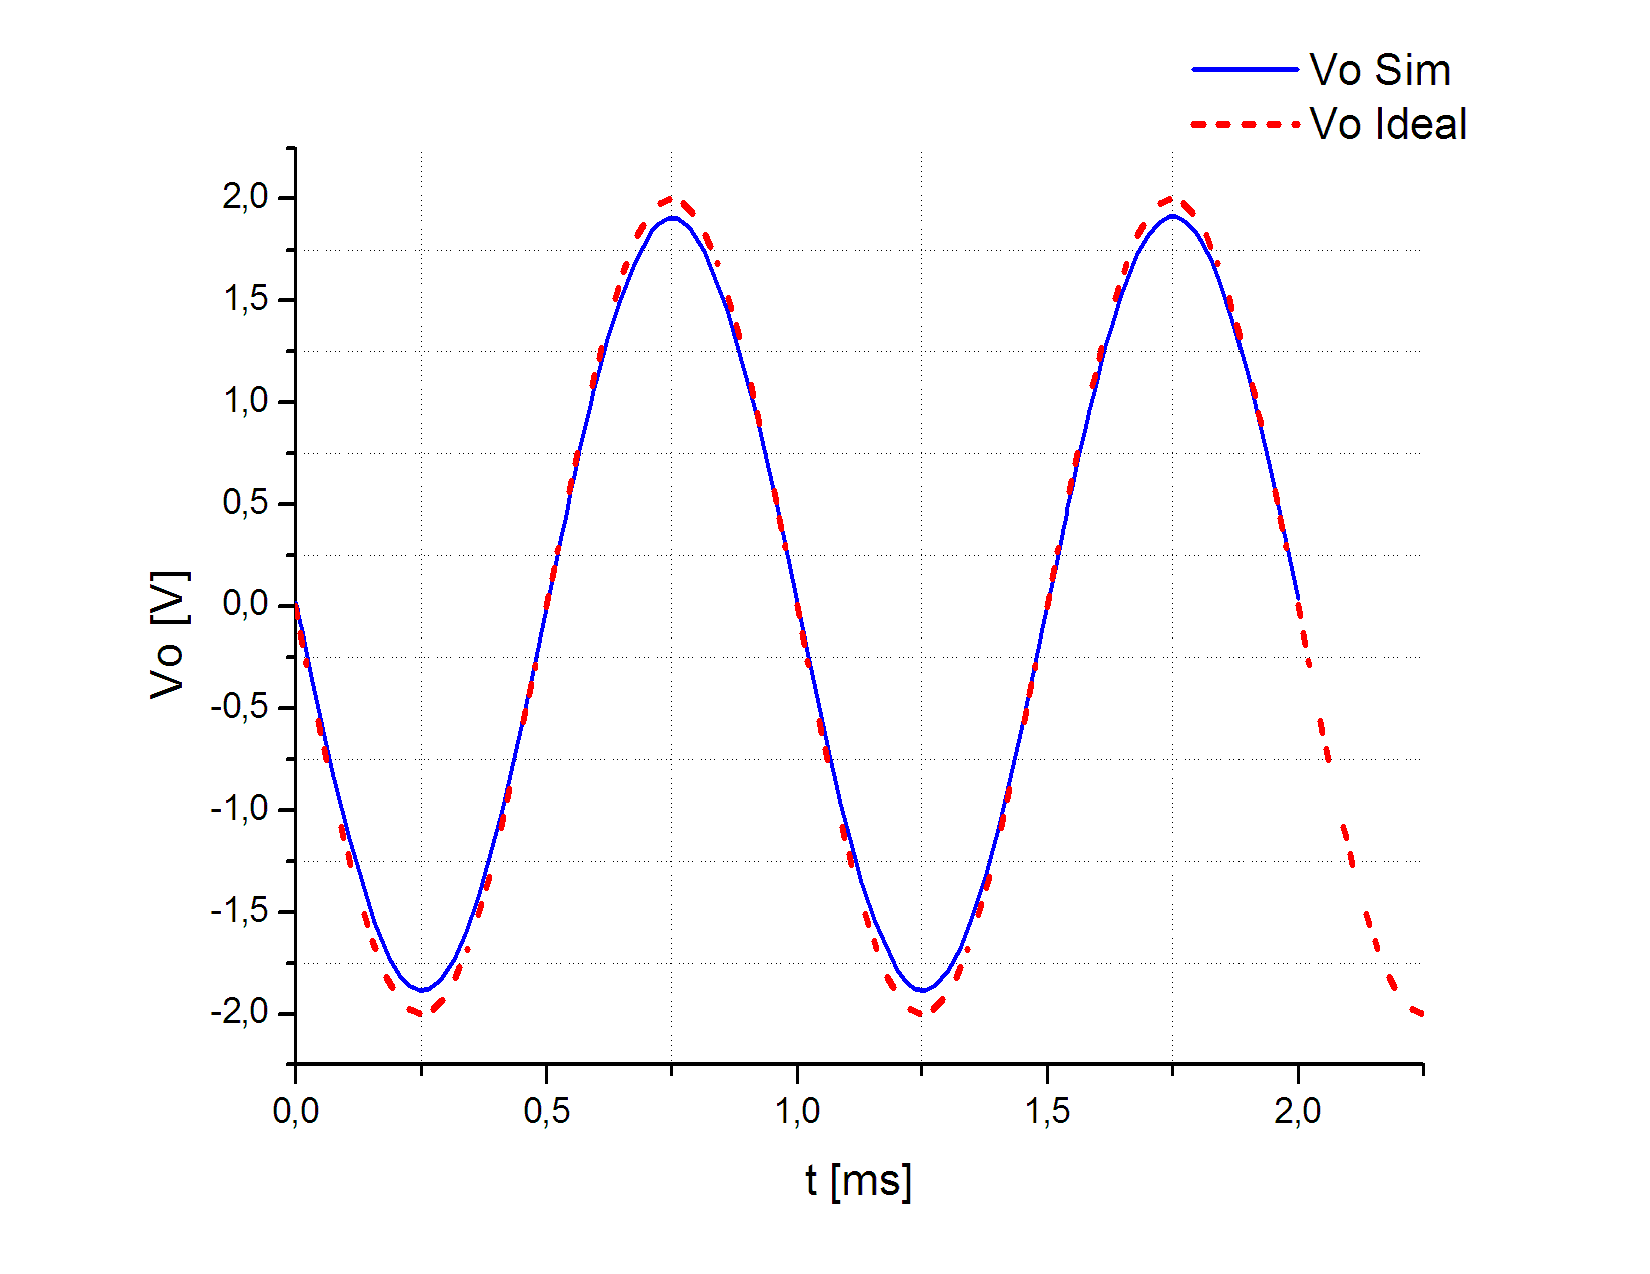
\includegraphics[width=0.8\textwidth]{gfxhernan/fig24.PNG}
  \caption{Señal ideal (rojo) comparada con la señal obtenida en la simulación (azul) para el caso a}
  \label{fig:multipl_simvsideal}
\end{figure}


En la simulación se agrega este circuito equivalente a la salida, en paralelo con la carga $R_{L}$, que será donde luego se medirá la señal en el osciloscopio. Finalmente se procede a simular el circuito, y se obtiene la señal de salida para los distintos valores de $R_{1}$ y $R_{2}$ como se ve en la Figura \ref{circ:multipl_banco_sim}.


\noindent$\blacktriangle$\textbf{ Observar que en el caso b) su valor se aparta más que en a) del predicho por el modelo ideal, al comenzar a influir el valor de $R_{i}$ del AO}

Para comparar las señales obtenidas en forma teórica (considerando al operacional como ideal) y las señales obtenidas mediante las simulaciones en Spice se colocarán ambas señales en un mismo gráfico con el fin de ver las similitudes y diferencias entre estas. Como puede verse en la Figura \ref{fig:multipl_simvsideal}, con la primera combinación de valores de $R_{1}$ y $R_{2}$ (caso a), lo que predice el circuito usando al AO como ideal es similar a lo obtenido en la simulación.


Si bien puede verse una pequeña diferencia de tensión, esto se debe a que en la simulación se utilizó un modelo de Thevenin del generador, por lo que en ésta se considera su resistencia interna.\\

Se procedió a medir la salida del AO bajo las mismas condiciones en el laboratorio. Como se puede observar en la Figura \ref{fig:multipl_a} se obtuvo una salida con los valores esperados.

\begin{figure}[H]
  \centering
      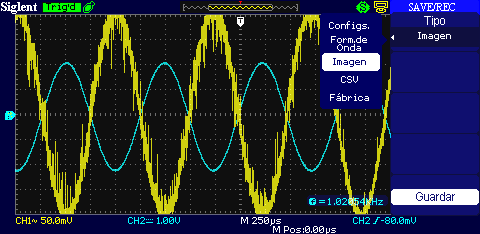
\includegraphics[width=0.6\textwidth]{gfxhernan/ampliparta.PNG}
  \caption{Pantalla de osciloscopio: señal de entrada (Canal 1) y señal de salida (Canal 2) obtenida en la medición}
  \label{fig:multipl_a}
\end{figure}

Trasladando los valores obtenidos en la medición y comparándolos con la salida predicha por el modelo ideal (Figura \ref{fig:multipl_a_idealvsmed}) puede verse que la tensión se invierte y es amplificada como fue estimado.

\begin{figure}[h]
  \centering
      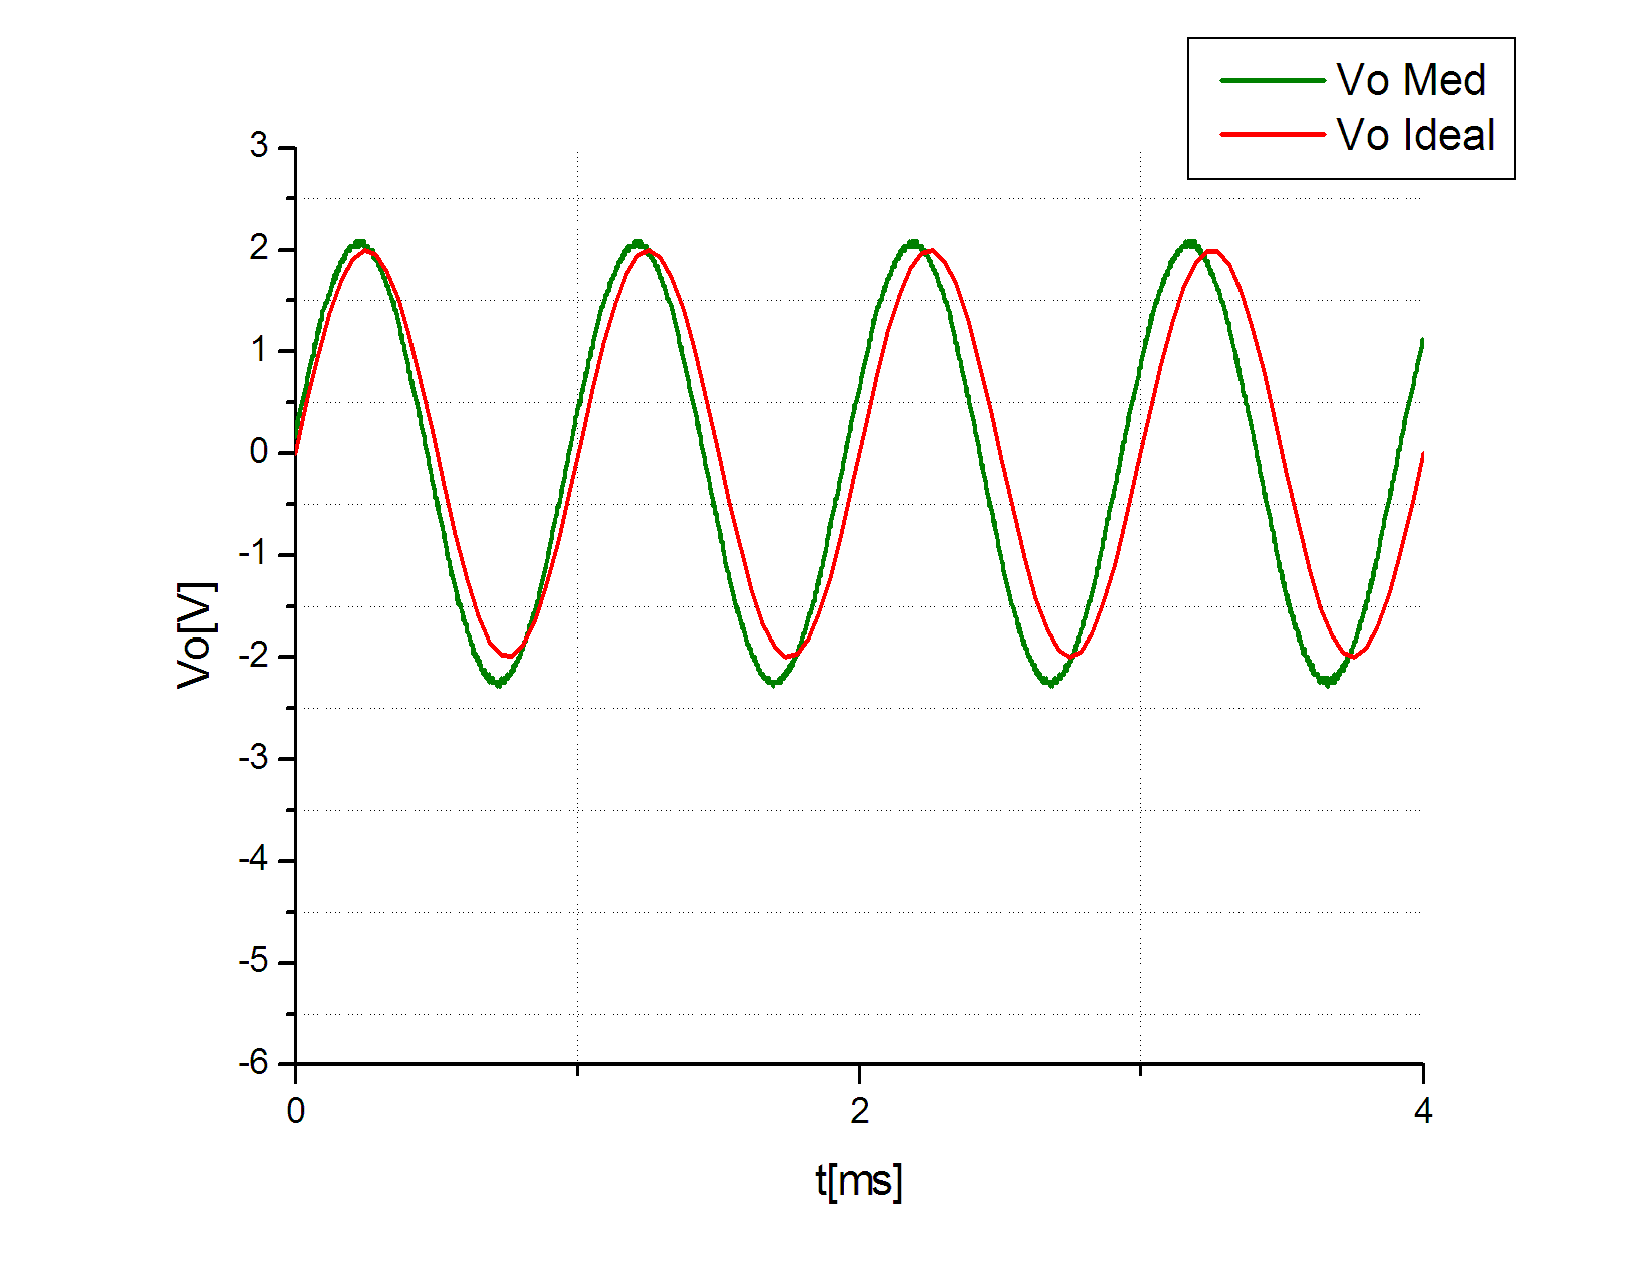
\includegraphics[width=0.7\textwidth]{gfxhernan/idealvsmedicionamplia.PNG}
  \caption{Señal ideal vs señal medida en el laboratorio}
  \label{fig:multipl_a_idealvsmed}
\end{figure}


%..............................CASO B, EL SIMULADOR DIVERGE......................................%
A pesar de que se pide comparar el caso a) con el b), se tuvo que obviar este paso puesto que al simular el punto b) el método numérico aplicado diverge en LTspice.
%Se pide comparar el caso a) con el caso b). Al simular el caso b) el LTSpice no logra simular el circuito, por lo que se obvió este paso.\\\\

\noindent$\blacktriangle$\textbf{ Para el caso b), modificar la base de tiempo hasta determinar cuál es la fuente de ruido que enmascara el valor útil a medir.}
\todo[inline, color=green!40]{No se si esto estará bien, chequear. - Santiago.

Quizás convenga agregar la imagen en la que se ve esa interferencia. No me acuerdo bien... Cómo era? el ruido viajaba por la masa del osciloscopio? - Luciano

Ahi esta la imágen, si haces 1/20ms da 50 Hz :) - Santiago}


La modularización de la señal por este ruido pudo ser captado cuando se cambió la fuente de trigger del osciloscopio a la tensión de línea.

Tras modificar la base de tiempo en el osciloscopio para apreciarlo en detalle, se pudo determinar que la fuente de dicha interferencia es la tensión de línea, lo que producía una convolución entre la señal deseada y otra de frecuencia aproximada de $50Hz$. Esto último puede apreciarse en la Figura \ref{fig:med_amplif_ruido}.

\begin{figure}[h]
  \centering
      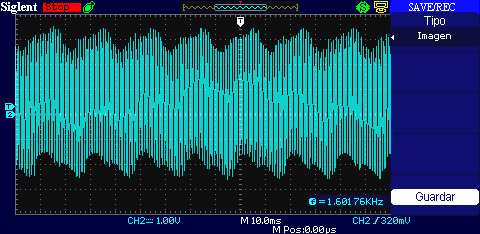
\includegraphics[width=0.7\textwidth]{gfxhernan/FIG_MED_Multipl_ruido.png}
  \caption{Reconocimiento de la tensión de línea como la fuente de interferencia.}
  \label{fig:med_amplif_ruido}
\end{figure}

\noindent$\blacktriangle$\textbf{ Observar que en el caso c) es imposible amplificar la señal a los valores que predice el modelo ideal, al alcanzarse los niveles de tensión máximos de funcionamiento, determinados por los valores de las tensiones de alimentación}

En el caso c, en donde $R_{1} = 1 k\Omega$ y $R_{2} = 1 M\Omega$ la señal de salida dada por el operacional ideal es de 200 V de amplitud. Analizando el gráfico de las dos señales claramente se observa que en la simulación esto no es así. Esto sucede debido a que la máxima tensión de funcionamiento esta dada por las tensiones de alimentación, en este caso 12V, y no se podrá superar ésta a la salida (en caso contrario estaríamos creando energía). Esto puede verse claramente en la Figura \ref{fig:multipl_c_idealvssim}:

\begin{figure}[h]
  \centering
      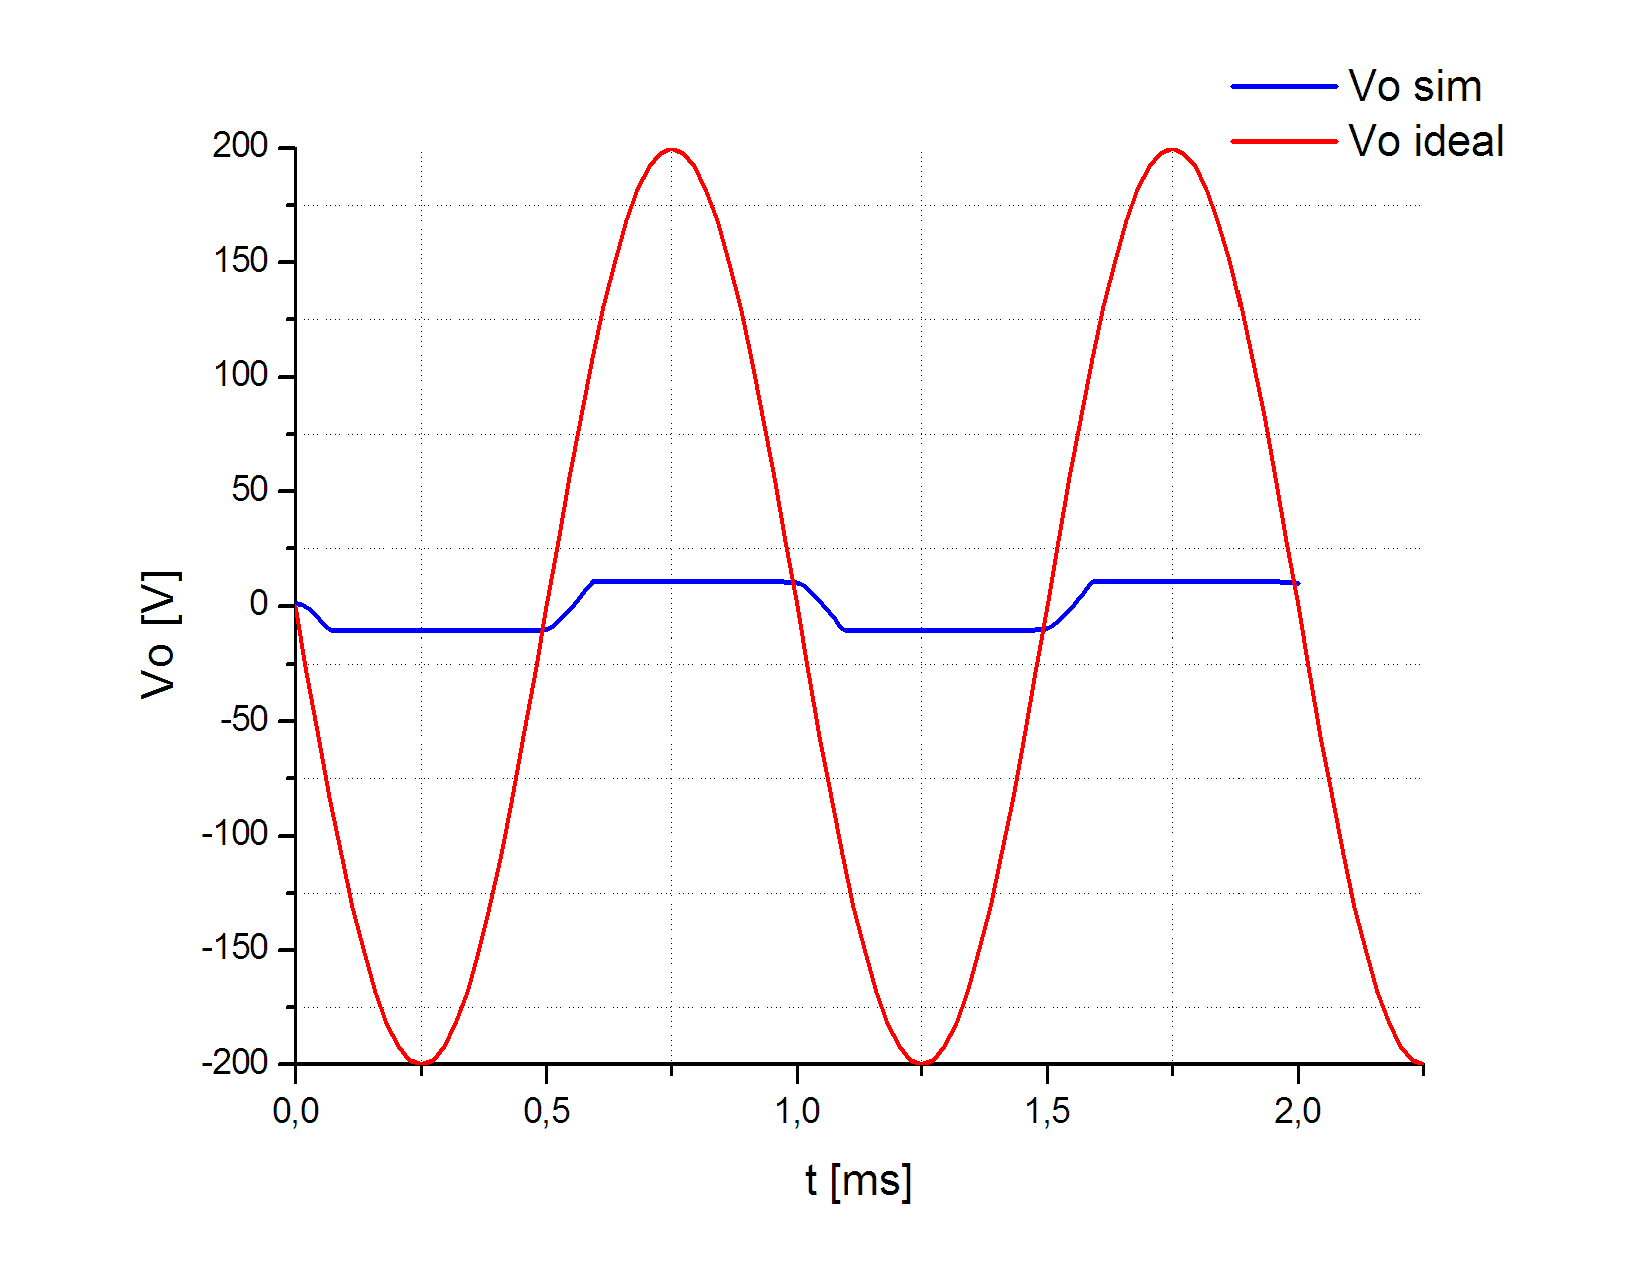
\includegraphics[width=0.6\textwidth]{gfxhernan/fig27.PNG}
  \caption{Señal ideal(rojo) comparada con la señal obtenida en la simulación (azul) para el caso c}
  \label{fig:multipl_c_idealvssim}
\end{figure}

Se procedió a la medición para este caso, obteniéndose el siguiente resultado en pantalla (Fig. \ref{fig:multipl_c_med}):

\begin{figure}[H]
  \centering
      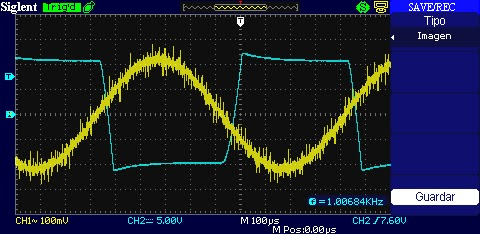
\includegraphics[width=0.6\textwidth]{gfxhernan/amplipartecmed.jpg}
  \caption{Pantalla de osciloscopio: puede verse que la salida se invierte pero no amplifica lo esperado por el modelo ideal, sino que aumenta como máximo 12 V}
  \label{fig:multipl_c_med}
\end{figure}

Como era de esperarse, no se logra la amplificación que predice el modelo ideal. Al trasladar los datos obtenidos mediante el osciloscopio y comparar con lo predicho por el AO (Fig. \ref{fig:multipl_idealvsmed}) se ve claramente que sucede lo que se observó en la simulación: el AO se satura, y al llegar a la tensión de alimentación en la salida corta y mantiene la tensión constante de 12 V todo el tiempo en el que la señal de entrada es tal que $v_{o}$ supera este valor.

\begin{figure}[H]
  \centering
      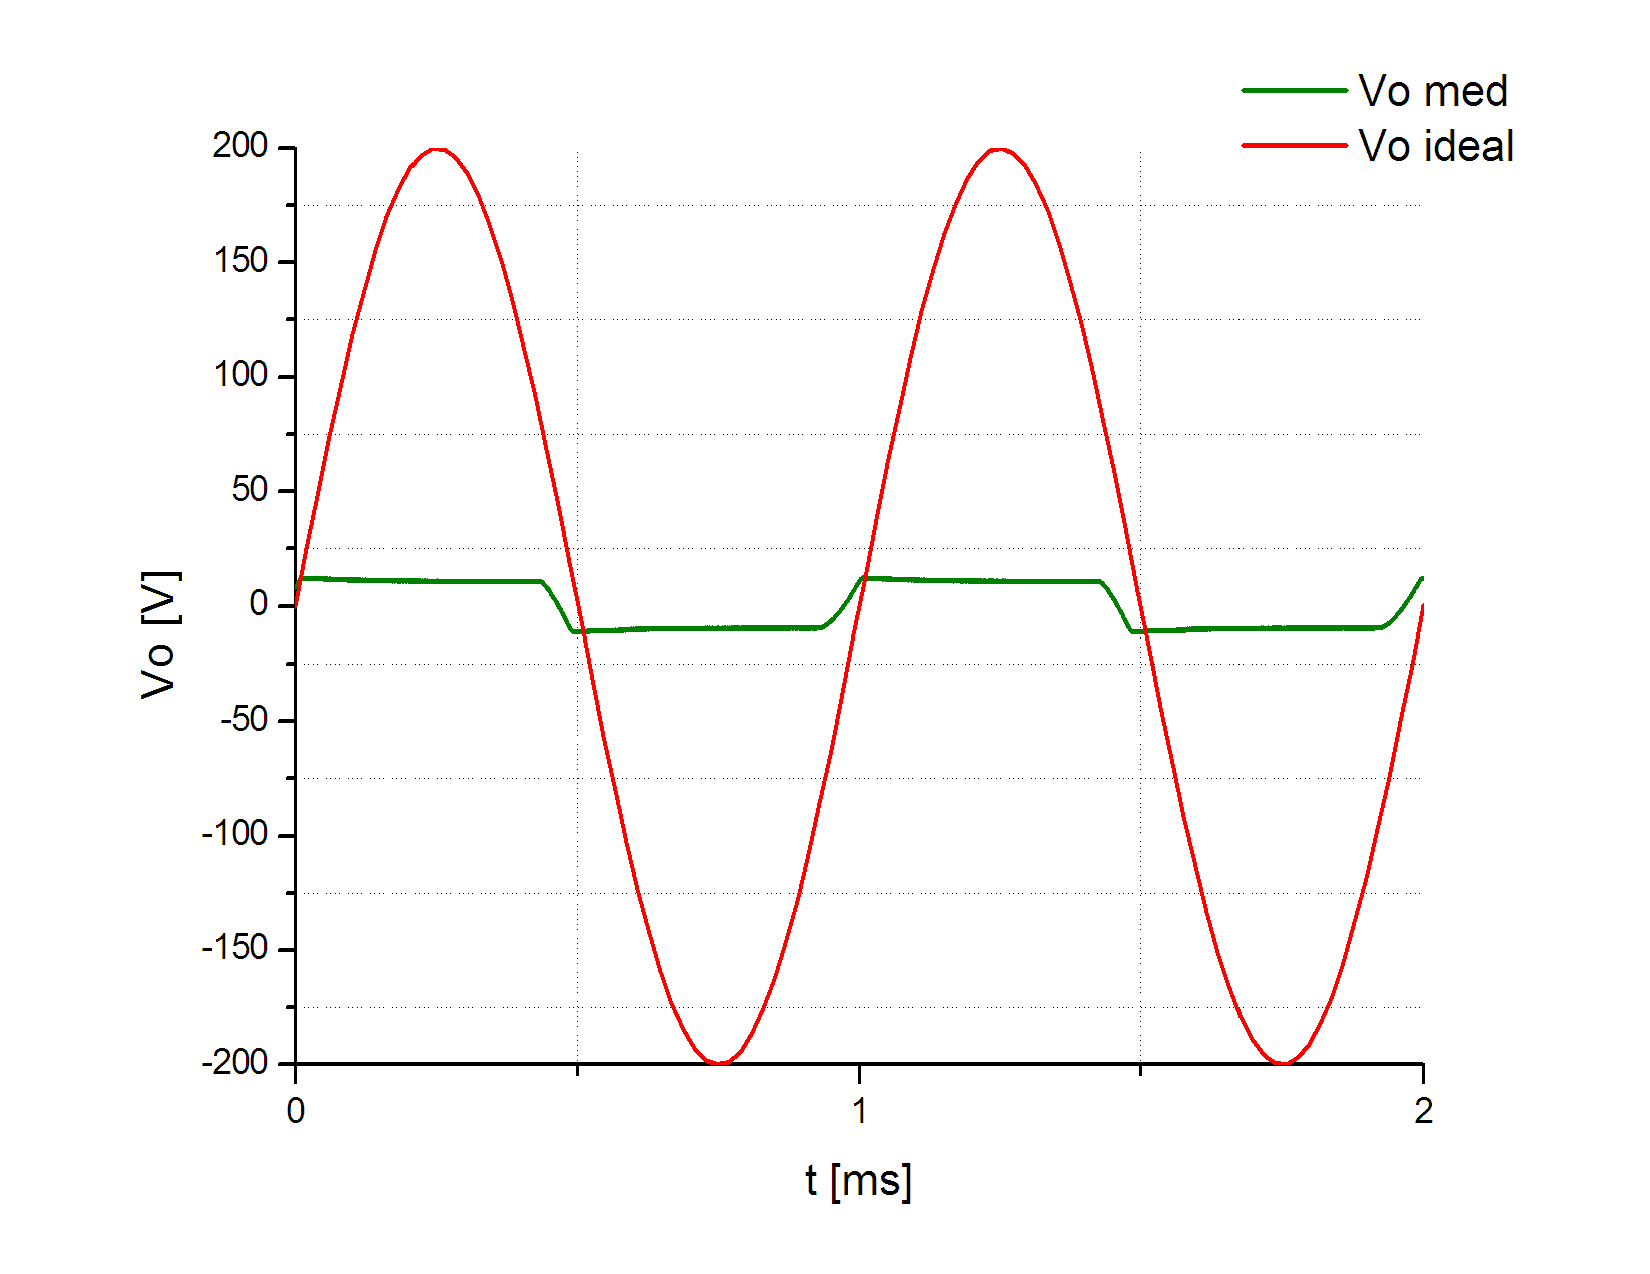
\includegraphics[width=0.6\textwidth]{gfxhernan/idealvsmedicionamplic.PNG}
  \caption{Señal ideal (rojo) comparada con la señal obtenida en las mediciones (verde) para el caso c}
  \label{fig:multipl_idealvsmed}
\end{figure}   

\noindent$\blacktriangle$\textbf{ Para el caso a), reemplazar la carga por otra de $10\Omega$ y ver que, si $R_{L}$ se hace comparable con la $R_{o}$ del AO, el valor de la amplificación de tensión se aparta del predicho por el modelo ideal}

Si ahora modificamos el valor de la carga $R_{L}$ por un valor comparable con $R_{o}$ (resistencia de salida del operacional) nos alejamos de lo predicho por el modelo ideal y por ello el operacional no amplifica lo esperado como se ve en la siguiente figura:

\begin{figure}[H]
  \centering
      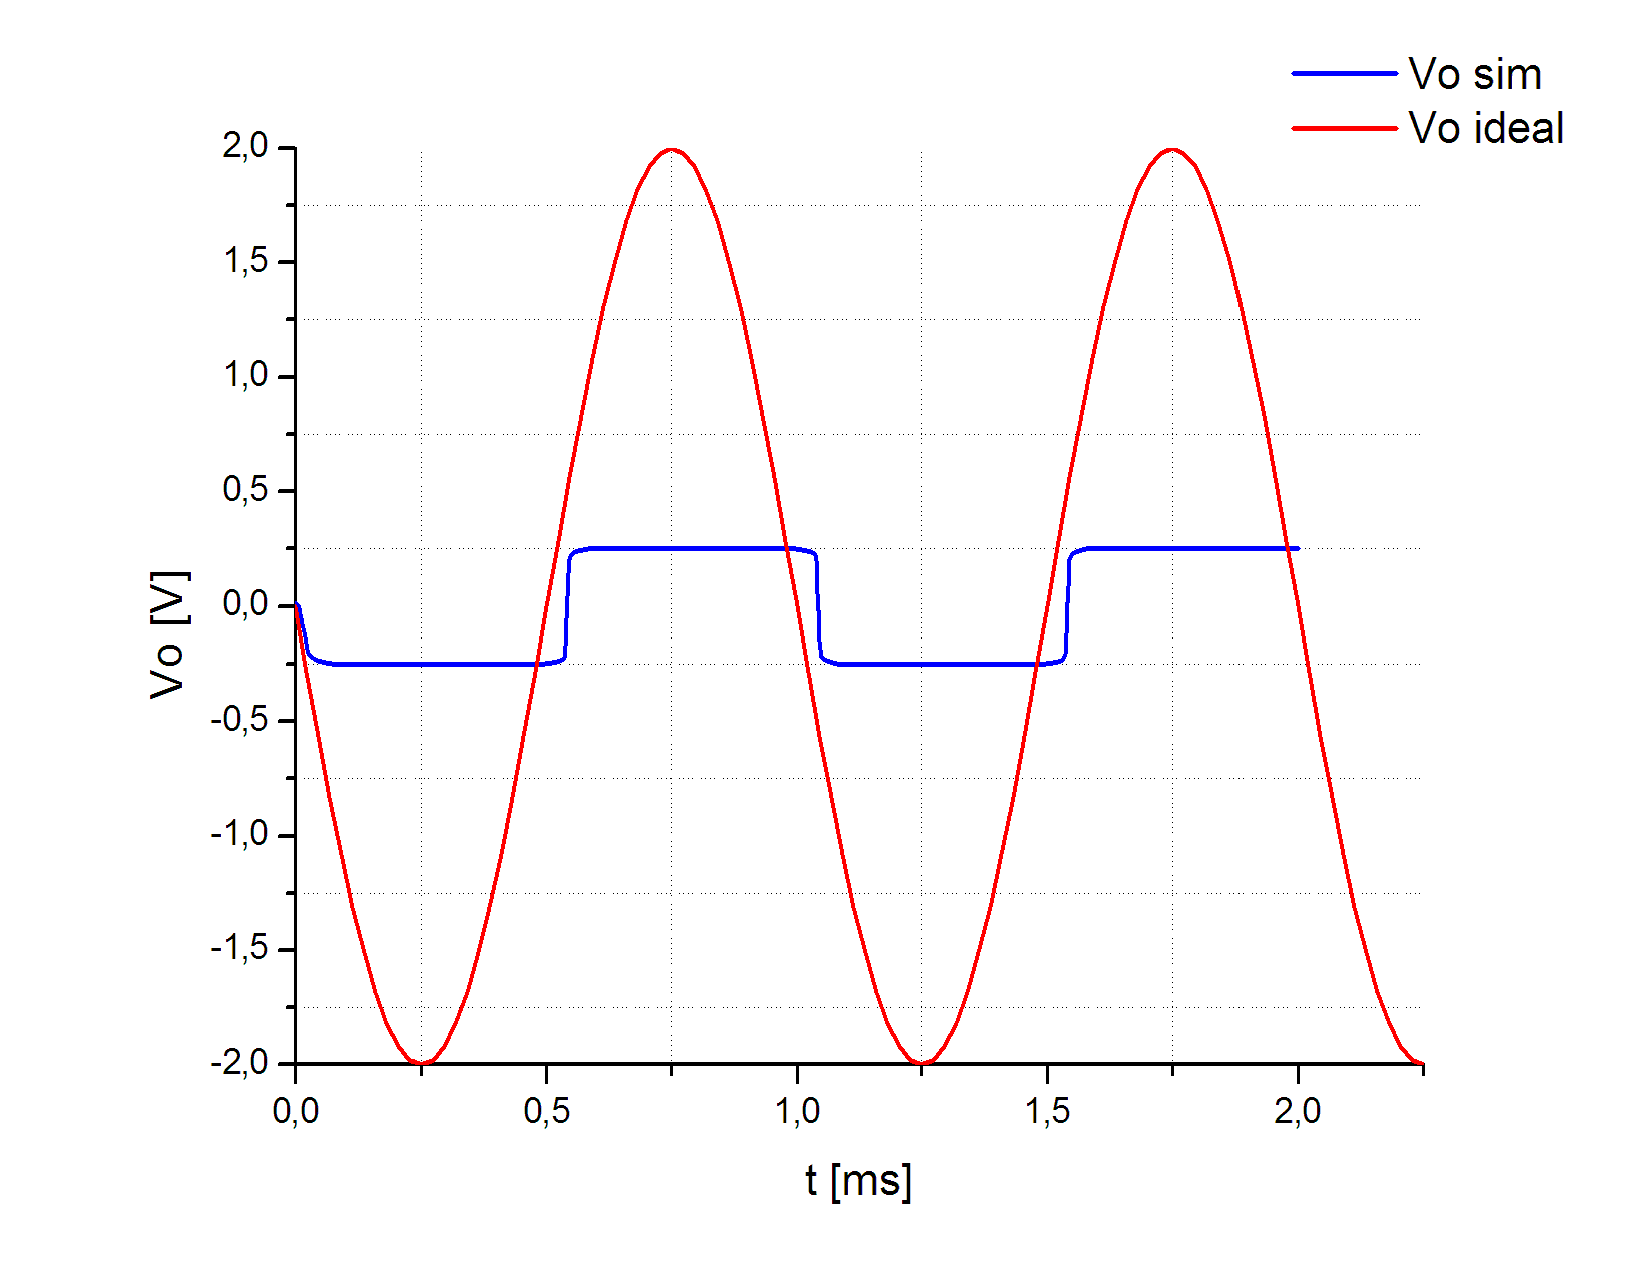
\includegraphics[width=0.8\textwidth]{gfxhernan/ampli4.PNG}
  \caption{Señal ideal (rojo) comparada con la señal obtenida en la simulación (azul) con $R_{L} = 10 \Omega$}
\end{figure}

Al ser la cargar $R_{L}$ comparable con la resistencia de salida, el AO debe entregar a la carga una corriente mayor a la máxima que puede ofrecer, esto provoca que se sature y no amplifique lo esperado.

\subsubsection{Variación de la tensión de salida en función de la frecuencia}
Vamos a proceder dejando la salida en vacío, es decir, sin ninguna carga conectada. Al momento de simular, debemos tener en cuenta nuevamente las influencia de los instrumentos. En este caso el osciloscopio y una punta 10x, las cuales agregan a la salida un circuito equivalente compuesto de una resistencia y una capacidad en paralelo:

\begin{figure}[H]
  \centering
      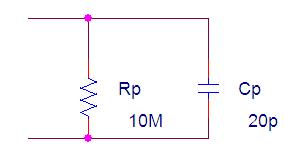
\includegraphics[width=0.5\textwidth]{gfx/puntax10.png}
  \caption{Circuito equivalente del osciloscopio junto a la punta 10X.}
\end{figure}

Lo que vamos a hacer, es fijar la tensión pico de entrada entre 50 mV y 100 mV e ir variando la frecuencia de la señal entre 0 Hz y 10 MHz, es decir, haremos un barrido en frecuencia mediante Spice.\\
En forma teórica, si analizamos el circuito de la Figura \ref{circ:multipl}, colocando el circuito equivalente de los instrumentos de medición, nos queda un circuito como el de la siguiente figura:

\begin{figure}[H]
  \centering
      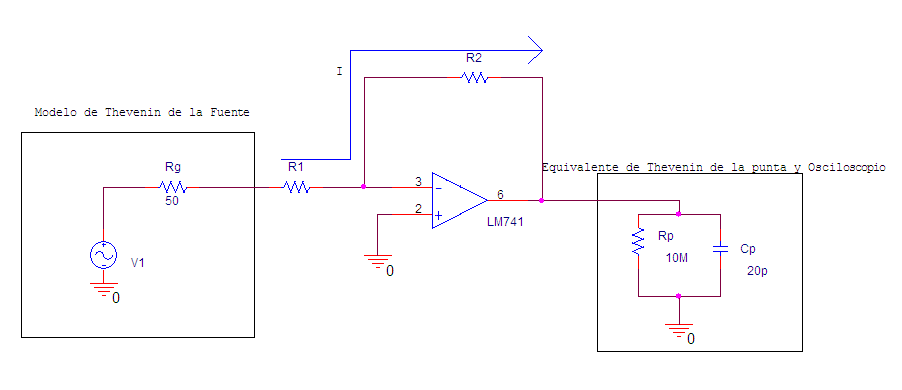
\includegraphics[width=0.8\textwidth]{gfxhernan/FIG28modif.PNG}
  \caption{Circuito utilizado para el barrido de frecuencia desde $0Hz$ a $10Mhz$.}
\end{figure}

Si suponemos al AO ideal, a corriente continua el capacitor $C_{1}$ actuaría como un circuito abierto ya que su impedancia da infinito, por lo que no circulará corriente por este. La tensión de salida se hallará de forma similar a como ya se hizo anteriormente. Aplicando en la entrada $v_{i}$ habrá en la salida $v_{o} = - i_{R1} R_{2}$. De esta manera, haciendo los cálculos se obtiene que en la salida habría - 500 mV con una entrada de 50 mV y - 1 V con una entrada de 100 mV.\\
A muy alta frecuencia el capacitor actuaría como un corto (su impedancia sería cero), y la tensión de salida sería 0 V ya que estaría en corto con tierra. Como no existe una frecuencia infinita podemos ver que pasaría si es muy grande, por ejemplo en este caso: 10 Mhz. A esta frecuencia la impedancia del capacitor $C_{1}$ nos da $0.0002 \Omega$ $\angle-90\degree$, es decir, casi cero en su módulo, por lo que se podría despreciar y decir que la salida queda cortocircuitada con tierra.
Lo que se espera entonces es que al ir variando la frecuencia desde 0 Hz a 10 Mhz la señal amplificada se vaya atenuando hasta llegar a cero mediante la frecuencia llega a los 10 Mhz. Para corroborar esto se hizo la simulación mediante Spice, usando el siguiente circuito:

\begin{figure}[H]
  \centering      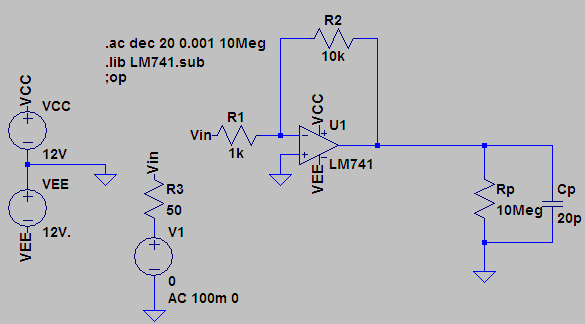
\includegraphics[width=0.8\textwidth]{gfxhernan/barrido2.PNG}
  \caption{Circuito utilizado para la simulación de barrido de frecuencia.}
\end{figure}


\begin{figure}[H]
  \centering      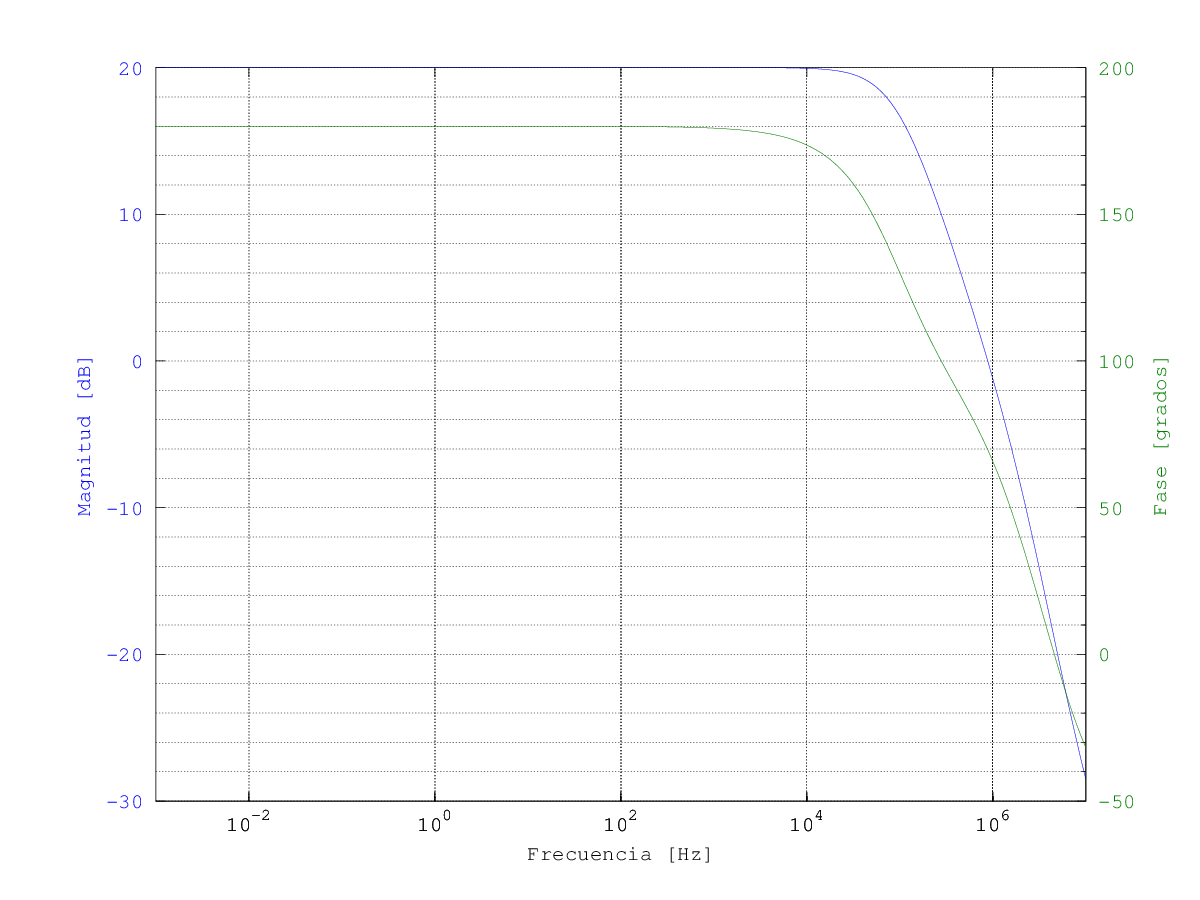
\includegraphics[width=0.8\textwidth]{gfxhernan/FIG_barrido_V_100.png}
  \caption{Simulación: Barrido de frecuencia.}
    \label{f:inv}
\end{figure}


Se realizó el correspondiente barrido de frecuencia en LTSpice para un solo valor de $\hat{V}_{i1}$, ya que por cuestión de tiempo en las mediciones se hizo para un solo valor: 100 mV. Se obtuvieron las siguientes curvas:\\

La frecuencia de corte por definición es aquel valor para el cual el módulo de la transferencia vale $\frac{1}{\sqrt{2}}$ multiplicado por el máximo valor que puede tomar el módulo de la transferencia. También es aquel valor para el cual la tensión cae 3 dB del valor máximo. Observando las curvas en el simulador, teniendo una amplitud de 100 mV se observa que a los 88 kHz caen 3 dB, por lo que la $f_{c} = 88 kHz$, aproximadamente.

%\begin{figure}[H]_punta1x
\begin{figure}[H]
  \centering      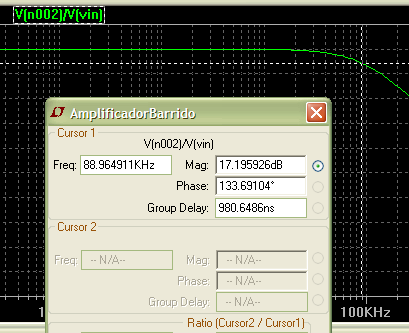
\includegraphics[width=0.6\textwidth]{gfxhernan/barrido1.PNG}
  \caption{Frecuencia para la cual caen 3 dB en la transferencia en el simulador}
\end{figure}

\noindent$\blacktriangle$\textbf{ ¿Por qué se debe medir también la tensión de entrada al obtener $f_{c}$ y no sólo ver si la tensión de salida cayó 3 dB?}

Debemos medir también la señal de entrada ya que hallamos la frecuencia de corte a partir en que caen 3 dB en la transferencia y no en la tensión de salida. La transferencia se la calcula como $H(jw) = \frac{V_{o}(jw)}{V_{i}(jw)}$, en el osciloscopio vamos viendo para distintas frecuencias los valores de $V_{i}$ y $V_{o}$ y hacemos su cociente para obtener la amplitud de la transferencia y luego poder trazar un gráfico.\\

\noindent$\blacktriangle$\textbf{ ¿Se esperaría medir el mismo valor de $f_{c}$ de utilizar la punta de prueba directa (1x)?}

Haciendo la misma medición, pero ahora utilizando una punta 1x, se ven cambios con respecto a la punta 10x en las simulaciones. Esto puede verse en las siguientes gráficas.\\

\begin{figure}[H]
  \centering      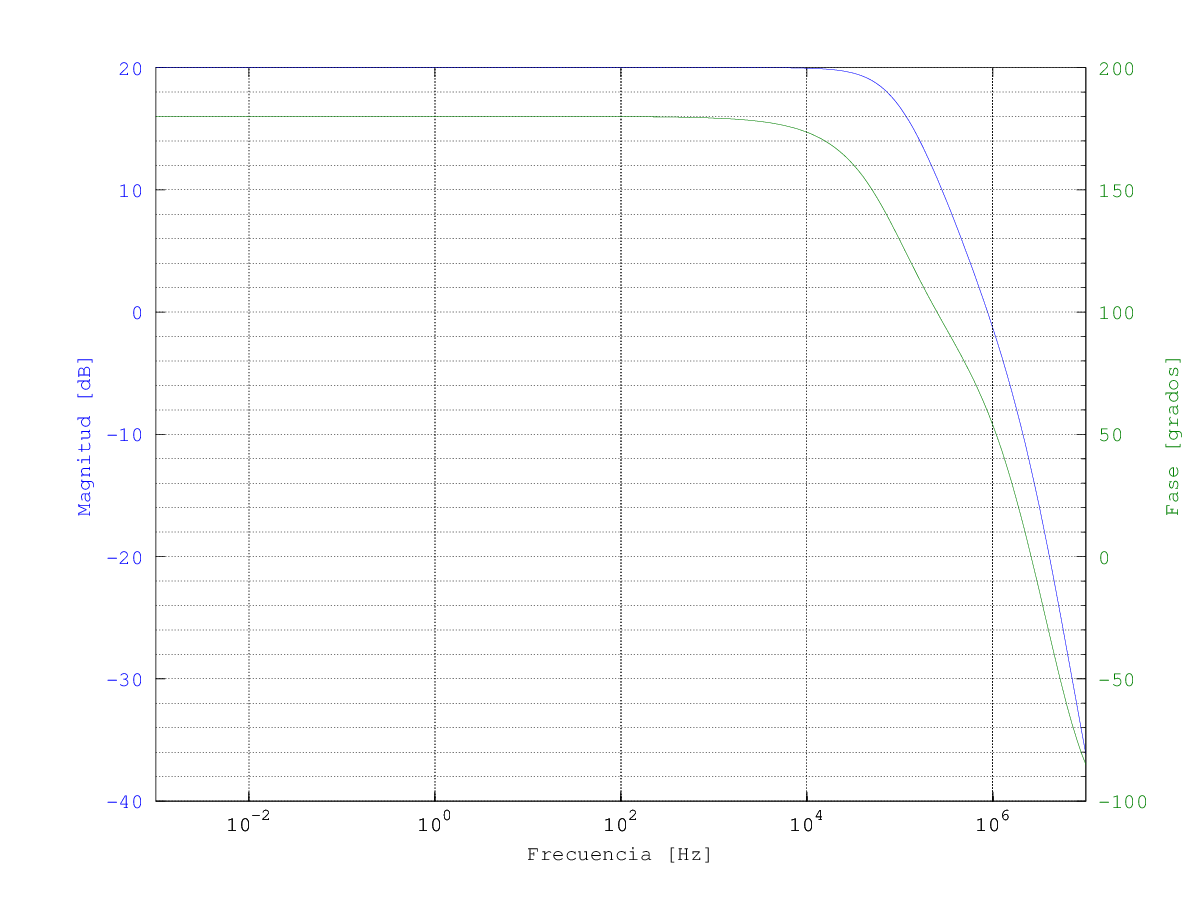
\includegraphics[width=0.8\textwidth]{gfxhernan/FIG_barrido_V_100_punta1x.png}
  \caption{Simulación: Barrido de frecuencia con punta 1x.}
\end{figure}

En este caso, para una amplitud de 100 mV a la entrada la frecuencia a la que caen 3 dB es aproximadamente a los $f_{c} = 92 kHz$. La frecuencia de corte aumentó casi $40kHz$.

%Antes habían escrito 4kHz, me parece que no es 4, sino que es 40 - fíjense si me equivoqué en lo que corregí - Lucho

\begin{figure}[H]
  \centering      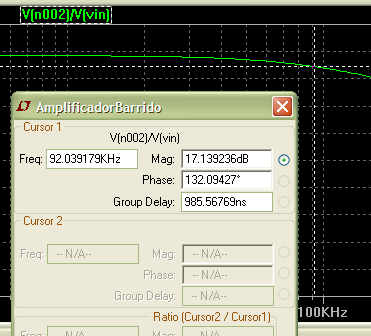
\includegraphics[width=0.6\textwidth]{gfxhernan/barrido3.PNG}
  \caption{Frecuencia para la cual caen 3 dB en la transferencia en el simulador utilizando punta directa (1X)}
\end{figure}

En caso de utilizar un tester digital, podríamos tener un problema. Estos instrumentos normalmente están fabricados para trabajar entre frecuencias encontradas en la red eléctrica (de 50 a 60 Hz). En este caso la frecuencia de entrada del circuito esta a 1 kHz por lo que el instrumento podría medir erróneamente  y mostrar valores erróneos en pantalla al estar trabajando a frecuencias para las cuales no fue diseñado.\\

\noindent$\blacktriangle$\textbf{ Aumentar la tensión de entrada más de 0,4 V. Verificar que a partir de esos niveles de tensión de entrada y frecuencia, el modelo del amplificador dejaría de predecir correctamente la forma de la tensión de salida}

Por último, se colocó a la entrada una amplitud mayor a 0,4 V. Se esperaba ver que las curvas cambiaran a medida que aumenta la frecuencia. Al simular esto no sucede, por lo que el error se le atribuye al modelo del operacional utilizado en las simulaciones.







\subsection{Integrador}


\subsubsection{Análisis teórico}


La siguiente etapa a analizar es el iintegrador compuesto por un operacional, una resistencia y un capacitor\footnote{Por no contar con el capacitor de $100 nF$ pedido en la consigna, el trabajo se realizó con uno de $100 pF$. Los resultados pueden ser extrapolados al otro caso.} como se muestra en la Figura \ref{circ:int1}.

\begin{figure}[H]
  \centering
      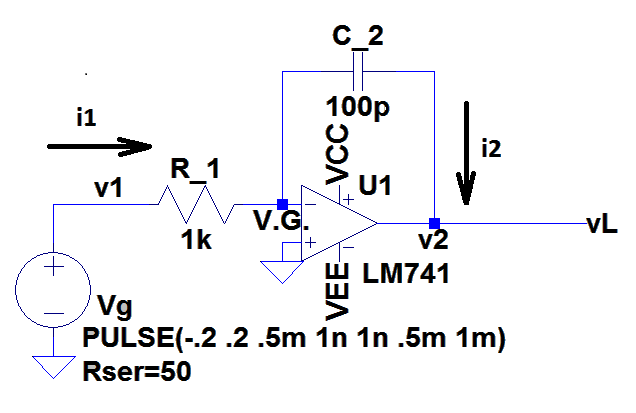
\includegraphics[width=0.5\textwidth]{gfx_22/circ_int1}
  \caption{Circuito integrador.}
  \label{circ:int1}
\end{figure}

Bajo la suposición de componentes ideales y generador con resistencia serie despreciable, se procede a realizar el análisis del circuito dado que $i_2(t) = \frac{q}{t}$.

Como $q = C.(V_{irtual}G_{round}-v_2(t)) \Rightarrow dq = d(C.(0V-v_2(t))) = -C.dv_2$.

Por lo que $i_2(t) = -C_2. \frac{d}{dt}v_2(t)$.

Asimismo, como la corriente que atraviesa a $C_2$ se considera igual a la que atraviesa a $R_1$ (por considerarse la resistencia de entrada del operacional infinita), se obtiene que $i_1(t) = \frac{v_1(t)}{R_1} = -C_2. \frac{dv_2(t)}{dt} = i_2(t)$.

Por ende,
\begin{equation}
v_o(t) = - \frac{1}{R_1.C_2}.\int_{-\infty}^{t}v_1(\tau)d\tau = -10^7\frac{1}{seg}.\int_{-\infty}^{t}v_1(\tau)d\tau
\end{equation}

La aplicación de este análisis tiene una serie de restricciones físicas del sistema, por lo que la salida no será la calculada para cualquier entrada. En principio, al ser el integrador un sistema inestable, cualquier variación de 0 puede disparar la salida ilimitadamente; pero las condiciones de borde impuestas por el sistema físico permite que $V_o$ solo pueda variar entre aproximadamente $\pm 11V$  definidos por la tensión de la fuente menos la caída sobre el operacional.



\subsubsection{Integrador con control de ganancia en continua}

Una variante del circuito anterior se obtiene al colocar una resistencia en paralelo al capacitor como se muestra en la Figura \ref{circ:int2}.

\begin{figure}[H]
  \centering
      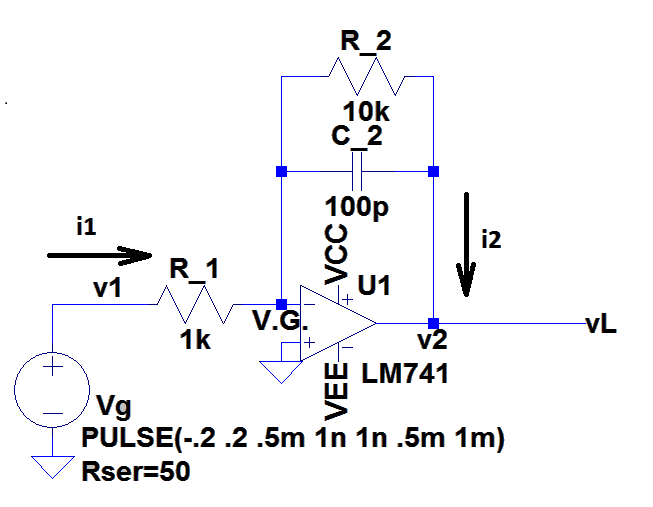
\includegraphics[width=0.5\textwidth]{gfx_22/circ_int2}
  \caption{Circuito integrador con control de ganancia en continua.}
  \label{circ:int2}
\end{figure}

Para este circuito, al hacer valer todas las condiciones anteriores de idealidad, también se puede hacer un análisis en el dominio de Laplace donde $ I(s) = \frac{V_1(s)}{R_1} = (V_{irtual}G_{round}-V_2(s)).\frac{1+s.C_2.R_2}{R_2}$.

Resultando en:

\begin{equation}
V_2(s) = - V_1(s) \frac{R_2}{R_1}.\frac{1}{1+s.C_2.R_2} = -\frac{1}{R_1.C_2}.\frac{1}{\frac{1}{R_2.C_2}+s} . V_1(s)
\end{equation}

Y su anti-transformada deriva en la siguiente ecuación diferencial:

\begin{equation}
\frac{d}{dt}v_2(t) = -\frac{v_2(t)}{R_2.C_2} -\frac{v_i(t)}{R_1.C_2} = -10^6\frac{1}{seg}.v_2(t) -10^7\frac{1}{seg}.v_1(t)
\end{equation}

En la Figura \ref{t:int2_RK4} presenta la respuesta a esta ODE para una entrada cuadrada de $0.2V$ pico. Esta ecuación diferencial fue resuelta por el método numérico Runge-Kutta de orden 4 con paso de $1ns$ a frecuencia $1MHz$.


\begin{figure}[H]
  \centering
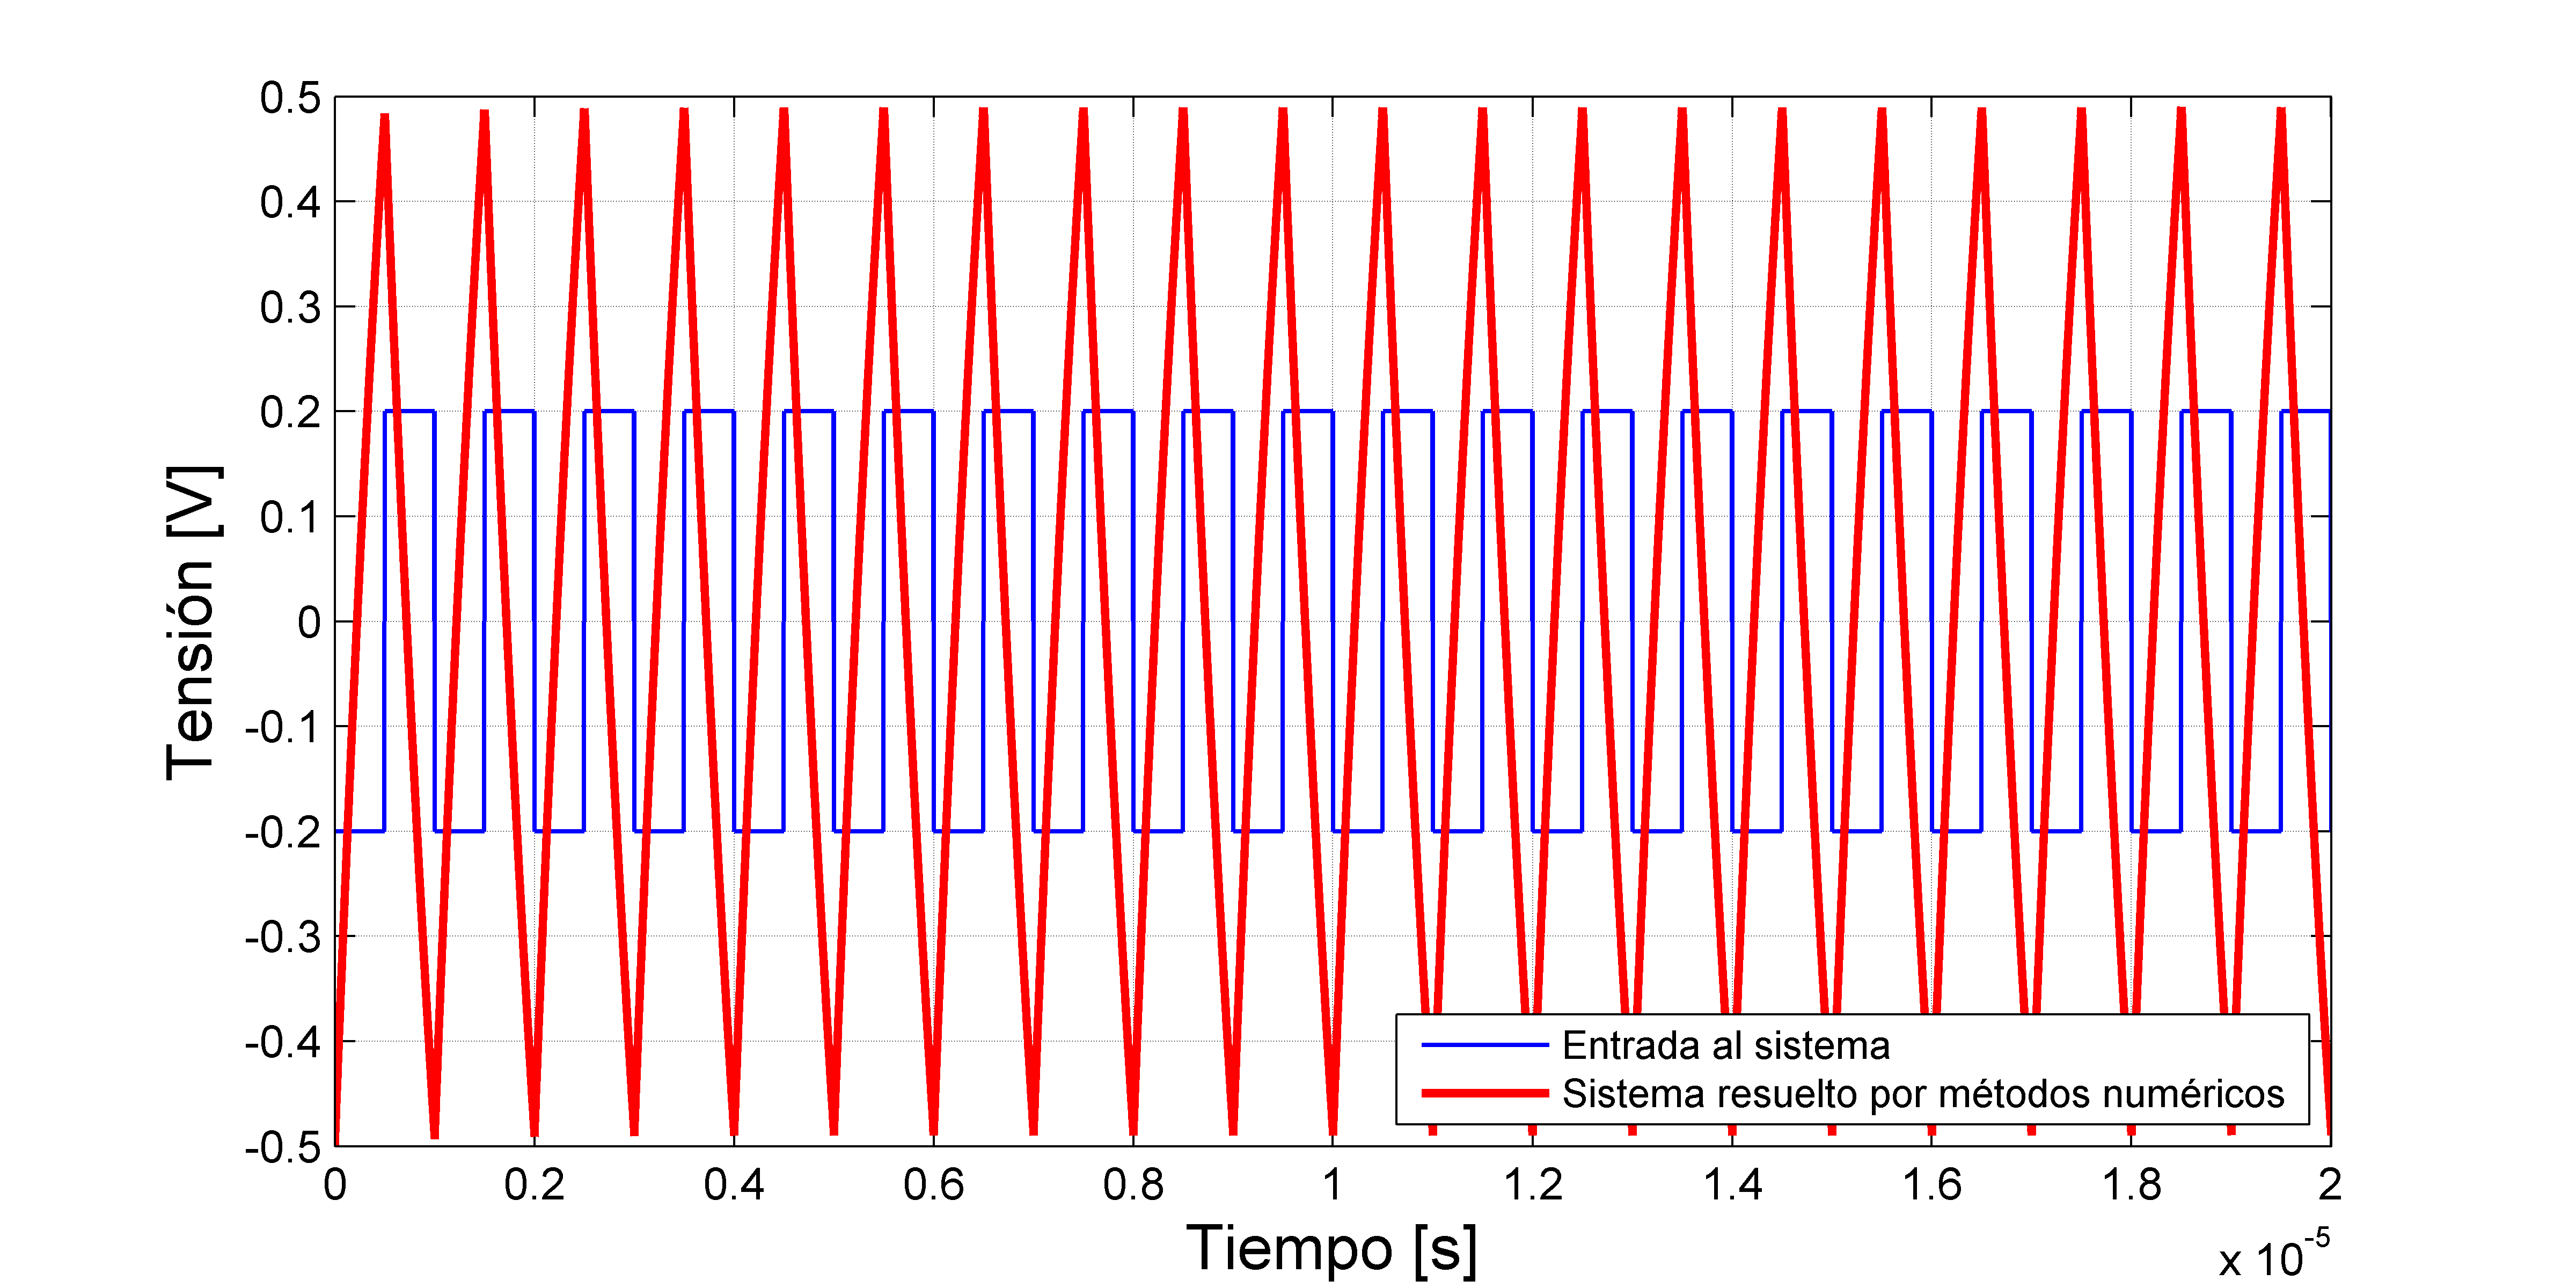
\includegraphics[width=.8\textwidth]{gfx_22/t_AMP2_RK4}
  \caption{Resolución por métodos numéricos de la ecuación diferencial de la respuesta temporal del circuito integrador con control de ganancia en continua.}
  \label{t:int2_RK4}
\end{figure}



\subsubsection{Simulaciones y respuesta de las etapas}

El integrador convencional tiene la respuesta en frecuencia mostrada en la Figura \ref{f:int1}, mientras que la simulación del segundo circuito se presenta el gráfico de la Figura \ref{f:int2}. Dichos gráficos muestran las simulaciones tanto sin carga como con los modelos de osciloscopio de la sección anterior con puntas $1x$ y $10x$.

\begin{figure}[H]
  \centering
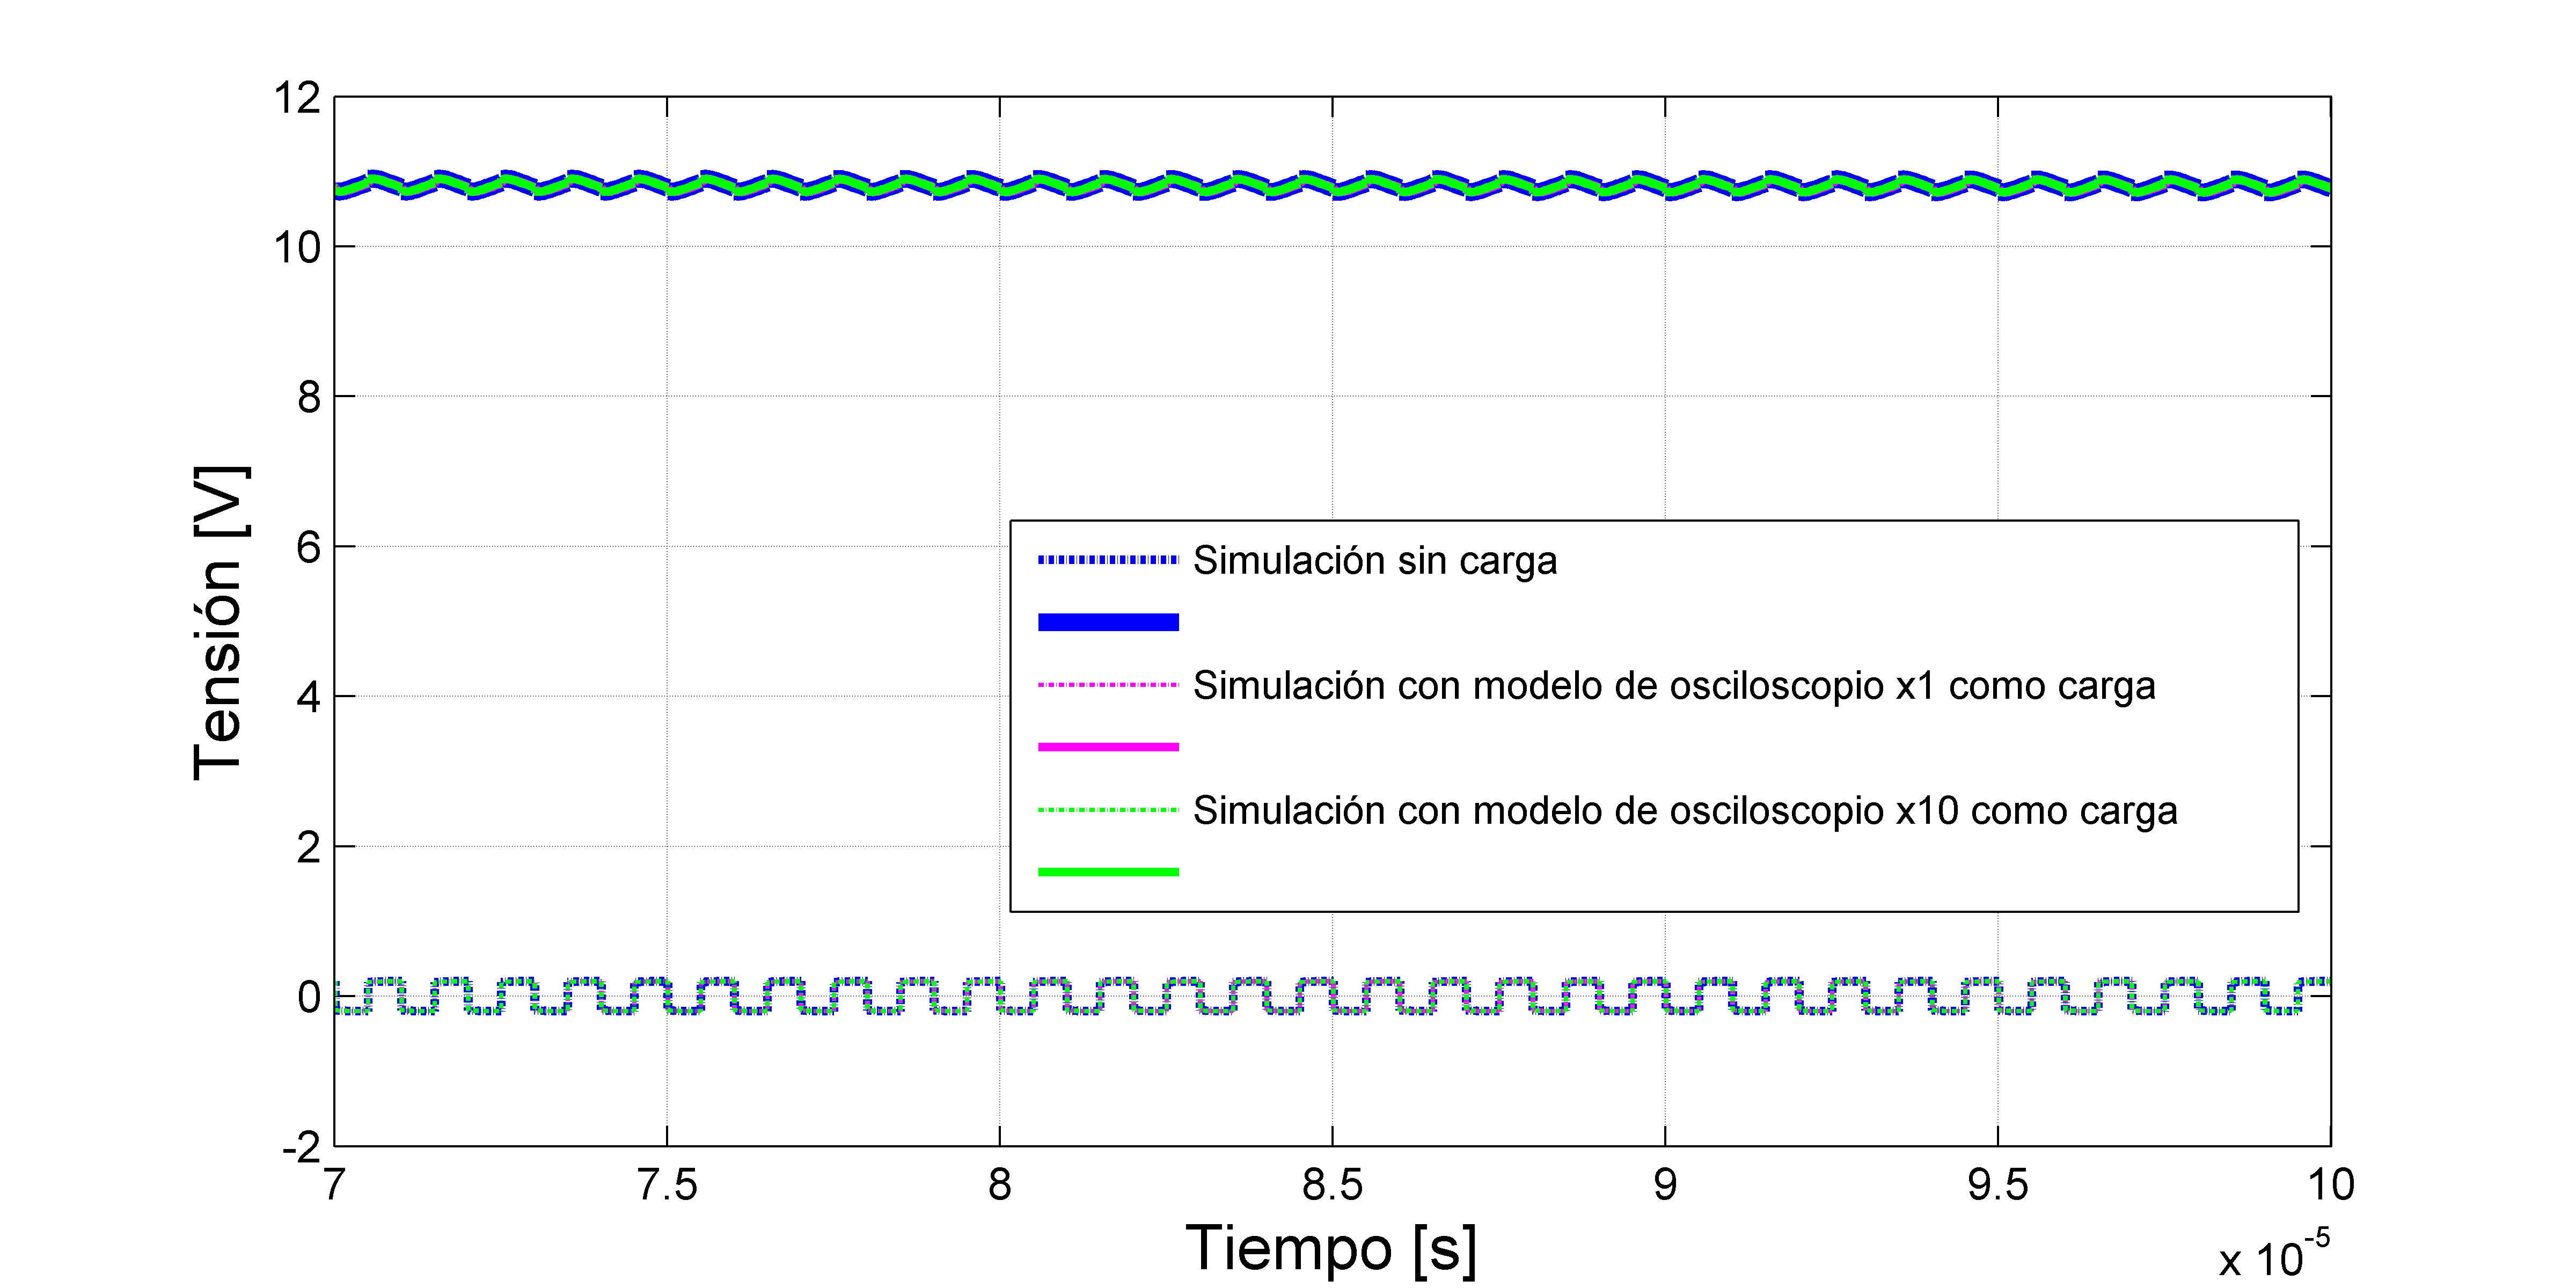
\includegraphics[width=1.1\textwidth]{gfx_22/INT1_T}
  \caption{Simulación de la respuesta temporal del circuito integrador. A baja frecuencia, para una entrada de $1V_p$, el sistema satura.}
  \label{t:int1}
\end{figure}

\begin{figure}[H]
  \centering
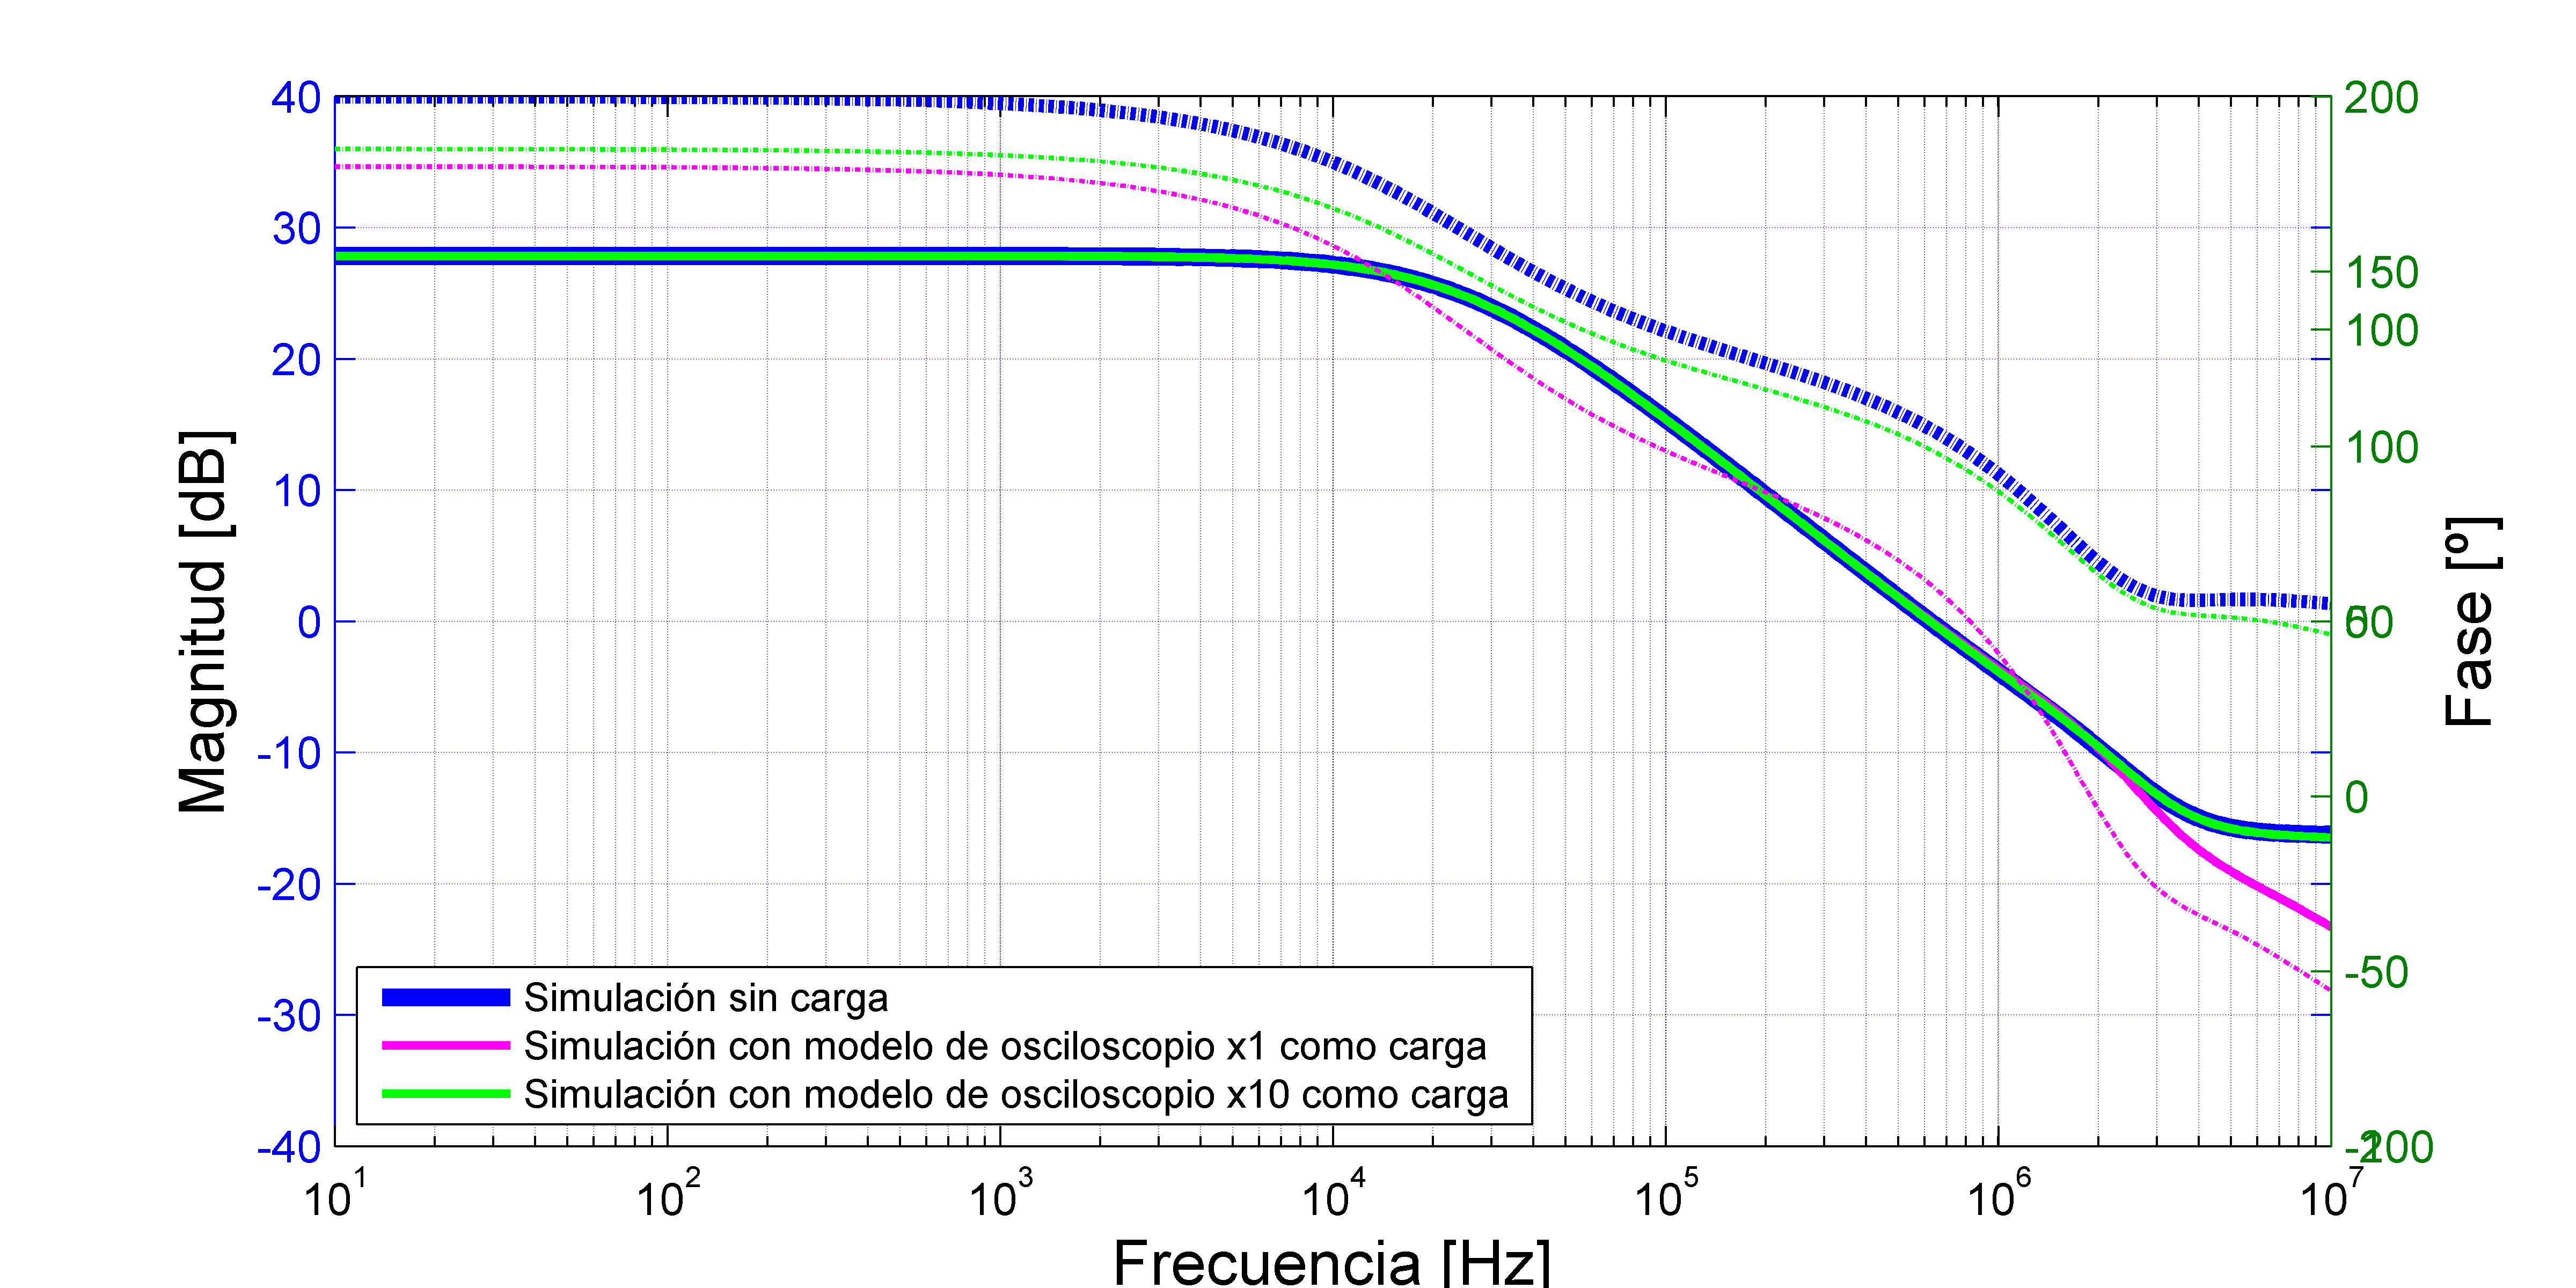
\includegraphics[width=1.1\textwidth]{gfx_22/INT1_F}
  \caption{Simulación de la respuesta en frecuencia del circuito integrador.}
  \label{f:int1}
\end{figure}



\begin{figure}[H]
  \centering
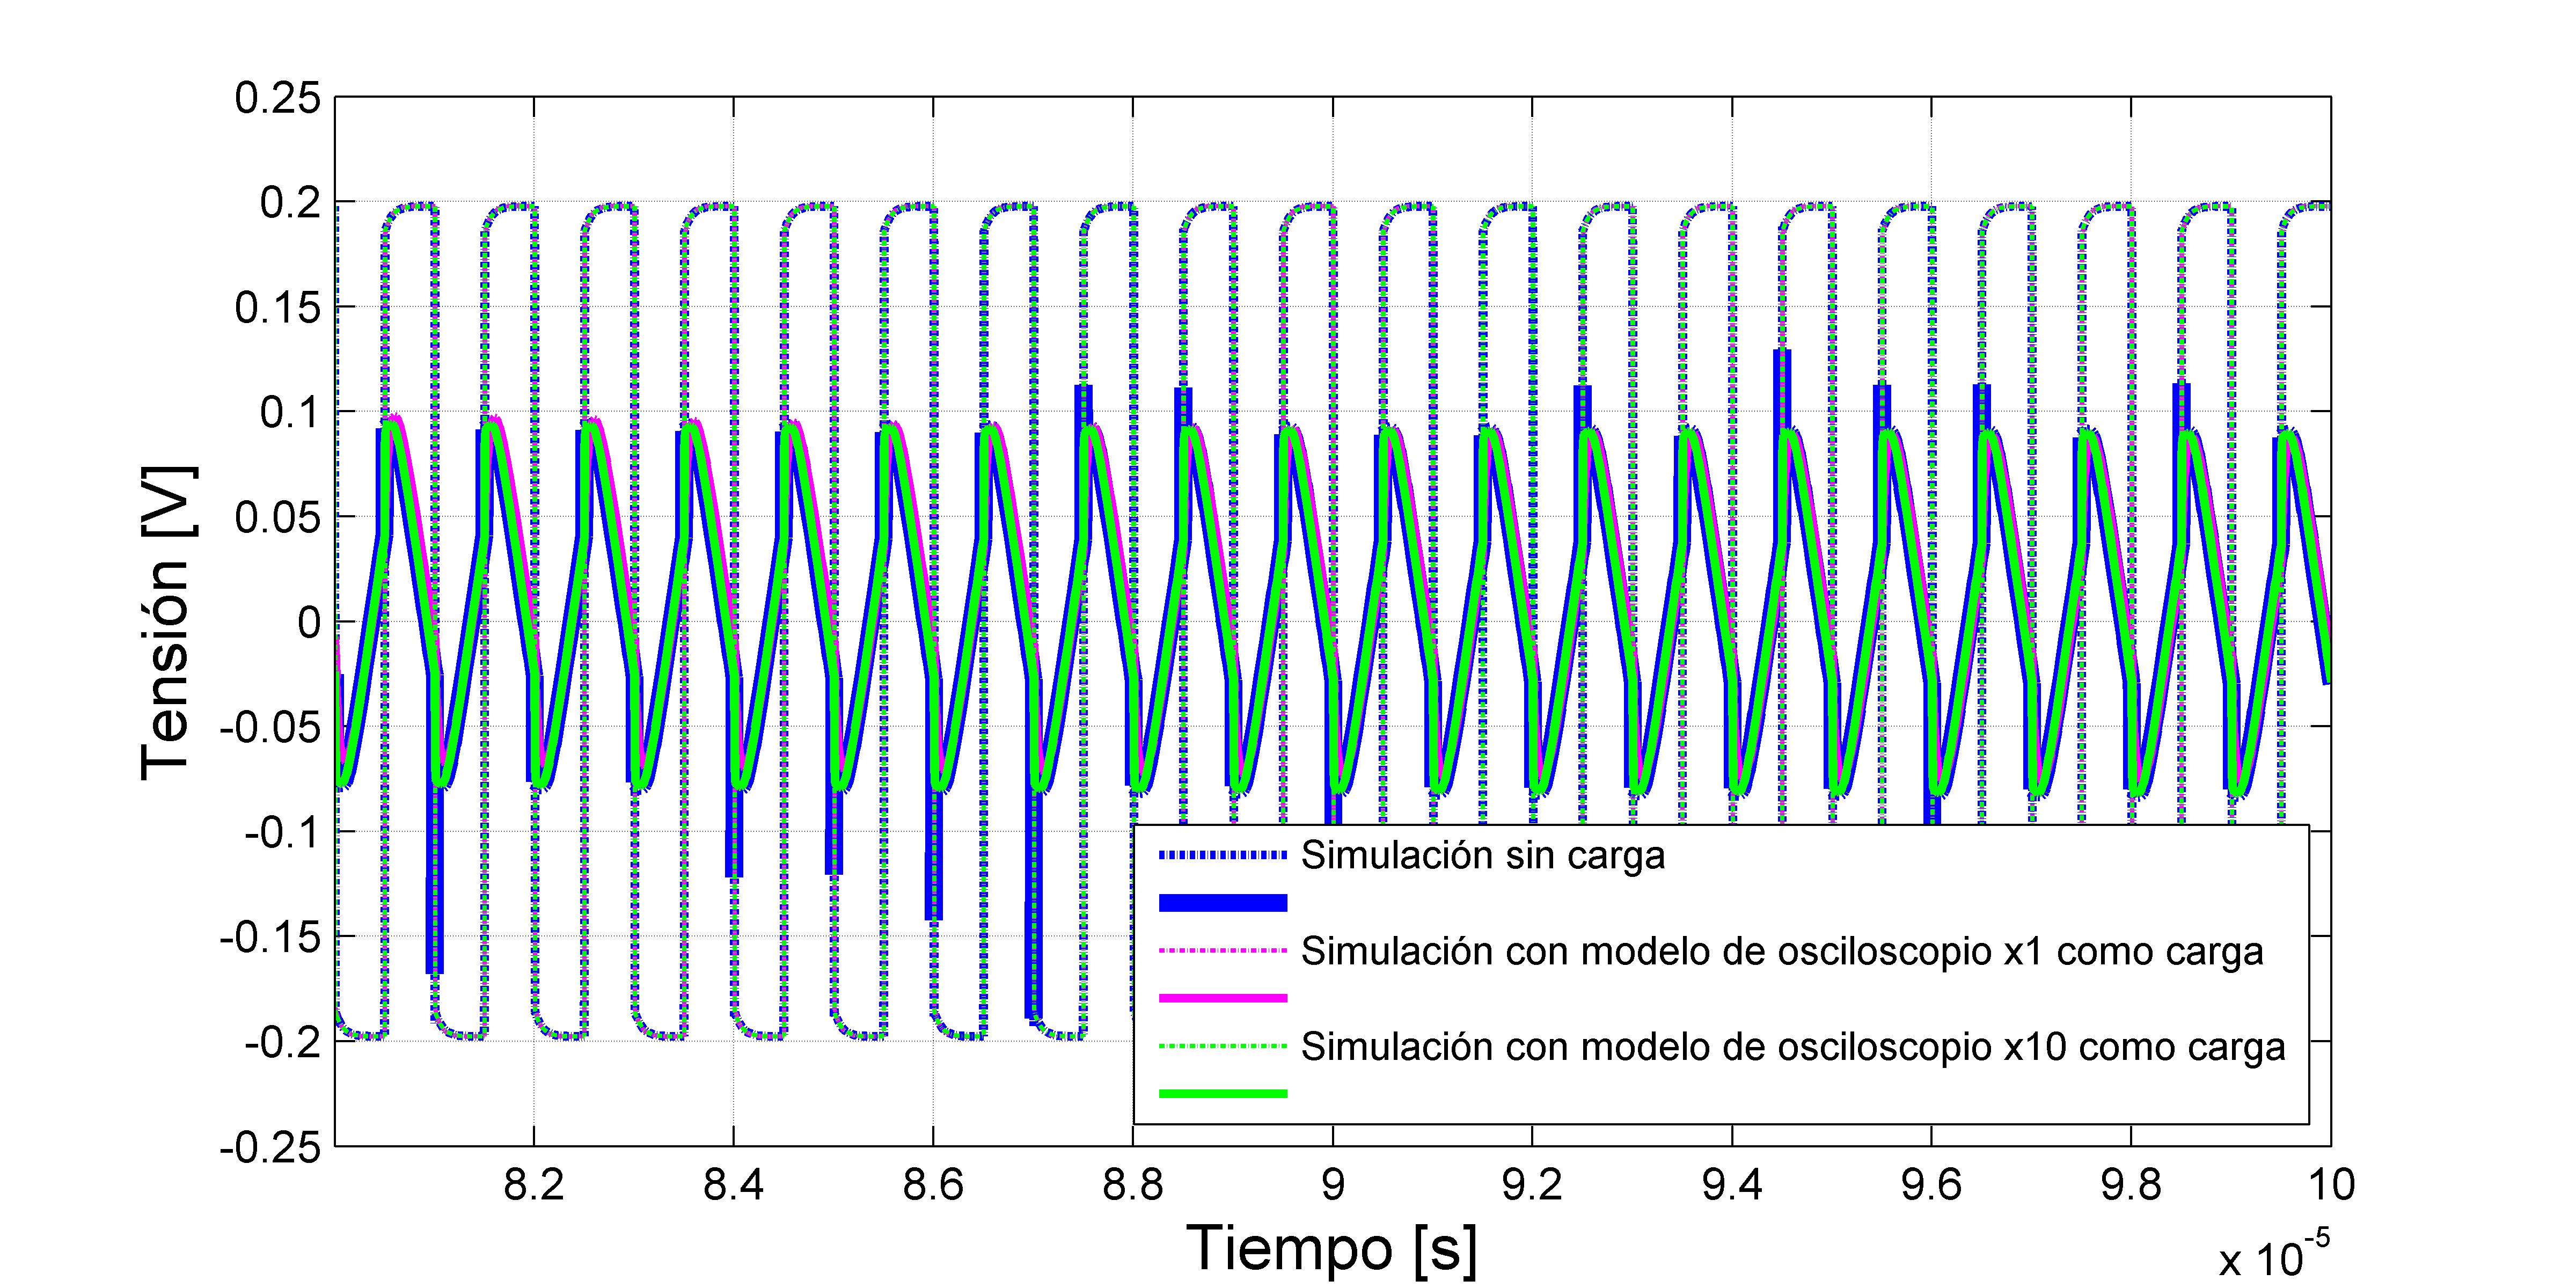
\includegraphics[width=1.1\textwidth]{gfx_22/INT2_T}
  \caption{Simulación de la respuesta temporal del circuito integrador con control de ganancia.}
  \label{t:int2}
\end{figure}

\begin{figure}[H]
  \centering
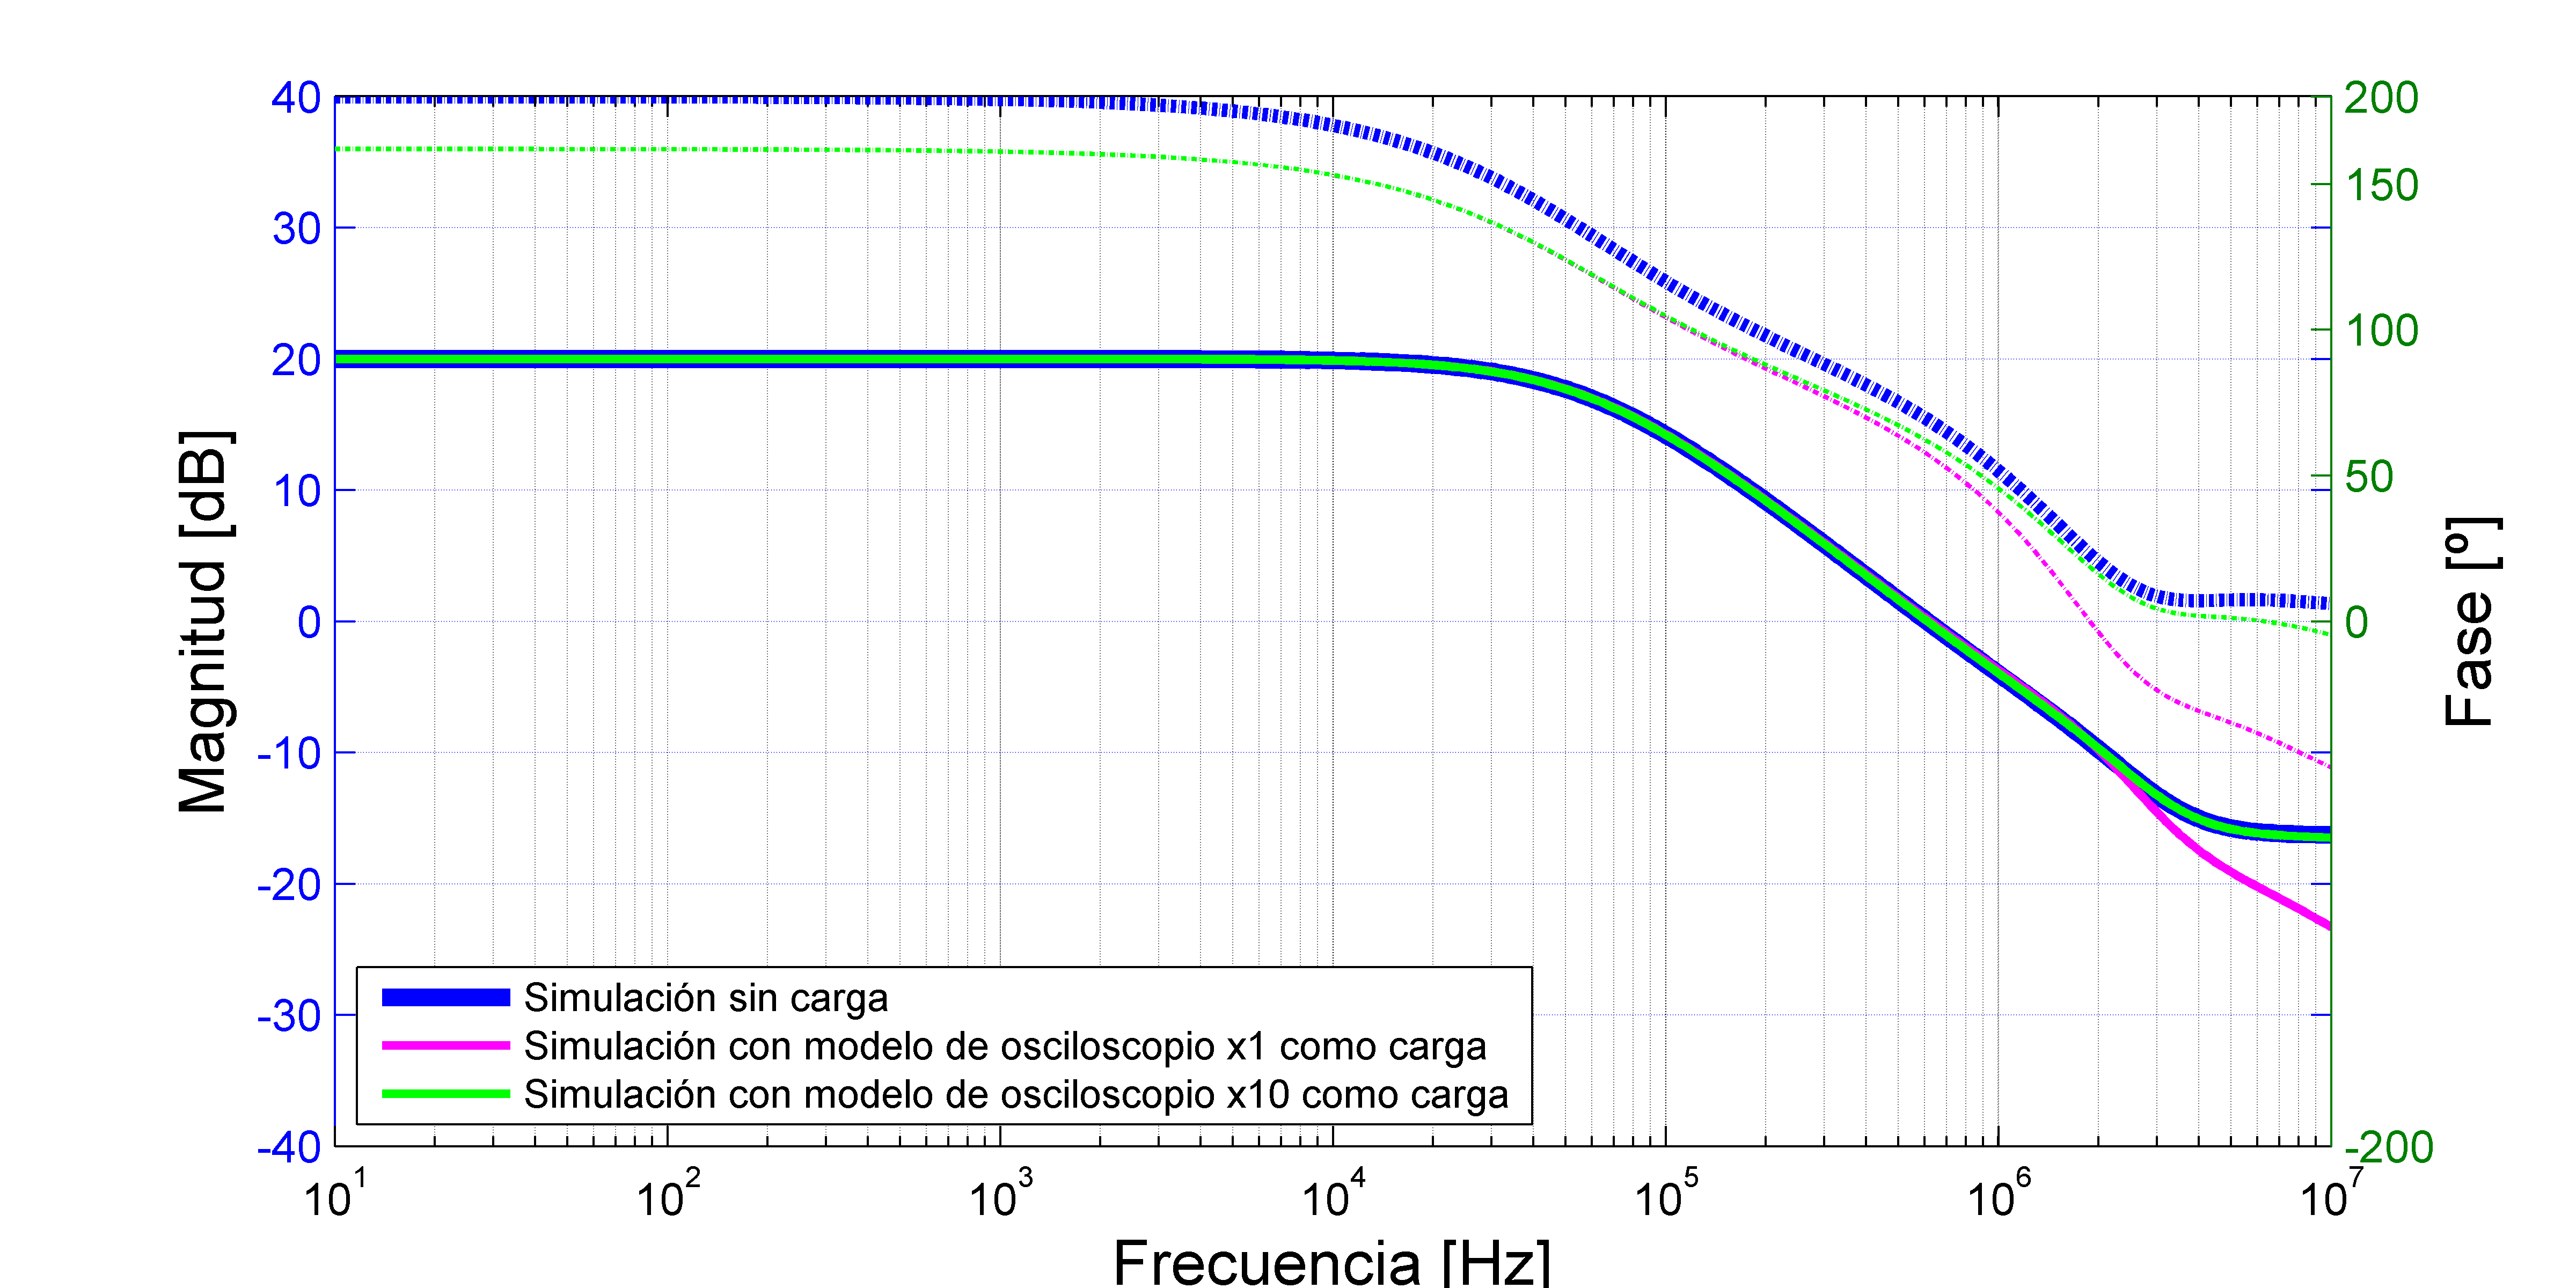
\includegraphics[width=1.1\textwidth]{gfx_22/INT2_F}
  \caption{Simulación de la respuesta en frecuencia del circuito integrador con control de ganancia.}
  \label{f:int2}
\end{figure}



El primer circuito satura en todo momento, ya que no tiene ningún tipo de compensación a la integración. Este sistema es altamente inestable.

Para compensar este problema, le es adicionada la $R_2$ en paralelo al $C_2$. Ésto impide que a bajas frecuencias el capacitor imponga una impedancia mucho más grande entre la entrada inversora y la salida del operacional, induciendo la transferencia $\frac{R_2}{R_1}$.




En la Figura \ref{f:int1} se ve cómo a frecuencias menores a $30kHz$ el circuito satura y la transferencia es limitada por los $\pm11V$, tal que $20.log(22V/1V)=26.8dB$. El polo de este primer circuito se encuentra a $0Hz$, pero la saturación del operacional no permite apreciarlo en el gráfico.

Como ha sido mencionado, la $R_2$ es introducida para limitar la ganancia a baja frecuencia, por lo que el polo es corrido a la frecuencia $\frac{1}{2\pi.R_2.C_2}$, permitiendo así introducir señales de amplitud hasta $10^{\frac{26.8dB-20dB}{20}}=2.2V_{pp}$ a frecuencias menores a la de corte antes de saturar el dispositivo.

%El polo fue transferido a $160kHz$, y esta es una frecuencia mayor a la frecuencia de corte del operacional (como fue visto en la Fig. \ref{f:inv}), por lo que la estimación realizada por el método numérico no se corresponderá con la medición.


%Aquí, debido al decrecimiento de la transferencia a partir de los $50kHz$, se puede apreciar que la simulación muestra que ambos circuitos poseen un polo no previsto por el análisis teórico. Esto hubiera sido posible visualizarlo si el análisis se realizaba considerando otro modelo en el que se contara con la impedancia de salida del amplificador operacional.




\subsubsection{Mediciones y comentarios}

Las mediciones de ambos circuitos se encuentran en las Figuras \ref{m:int1} y \ref{m:int2}, mientras que en la Figura \ref{mf:int2} se presenta la respuesta en frecuencia del segundo y su comparación contra la simulación.


Se puede apreciar que la frecuencia de corte del circuito medido se encuentra entre $90kHz$ y $100kHz$, ya que la amplitud máxima alcanzada es $20.441dB$, y en el rango mencionado se obtienen $3dB$ menos.


En ambas figuras sobre el dominio temporal se aprecia la integración realizada por el sistema. El período de crecimiento se encuentra en el semiciclo negativo de la señal cuadrada de entrada debido a la inversión que también ejecuta la etapa.


\noindent$\blacktriangle$\textbf{ ¿Cómo influye el ancho de banda del osciloscopio en el valor medido del tiempo de crecimiento?}

No es apreciable una diferencia en el ancho de banda del circuito, pero a  frecuencias mayores se identifica un gradiente mayor con el cual decrece la respuesta cuando la punta del osciloscopio se encuentra en $1x$.




\begin{figure}[H]
  \centering
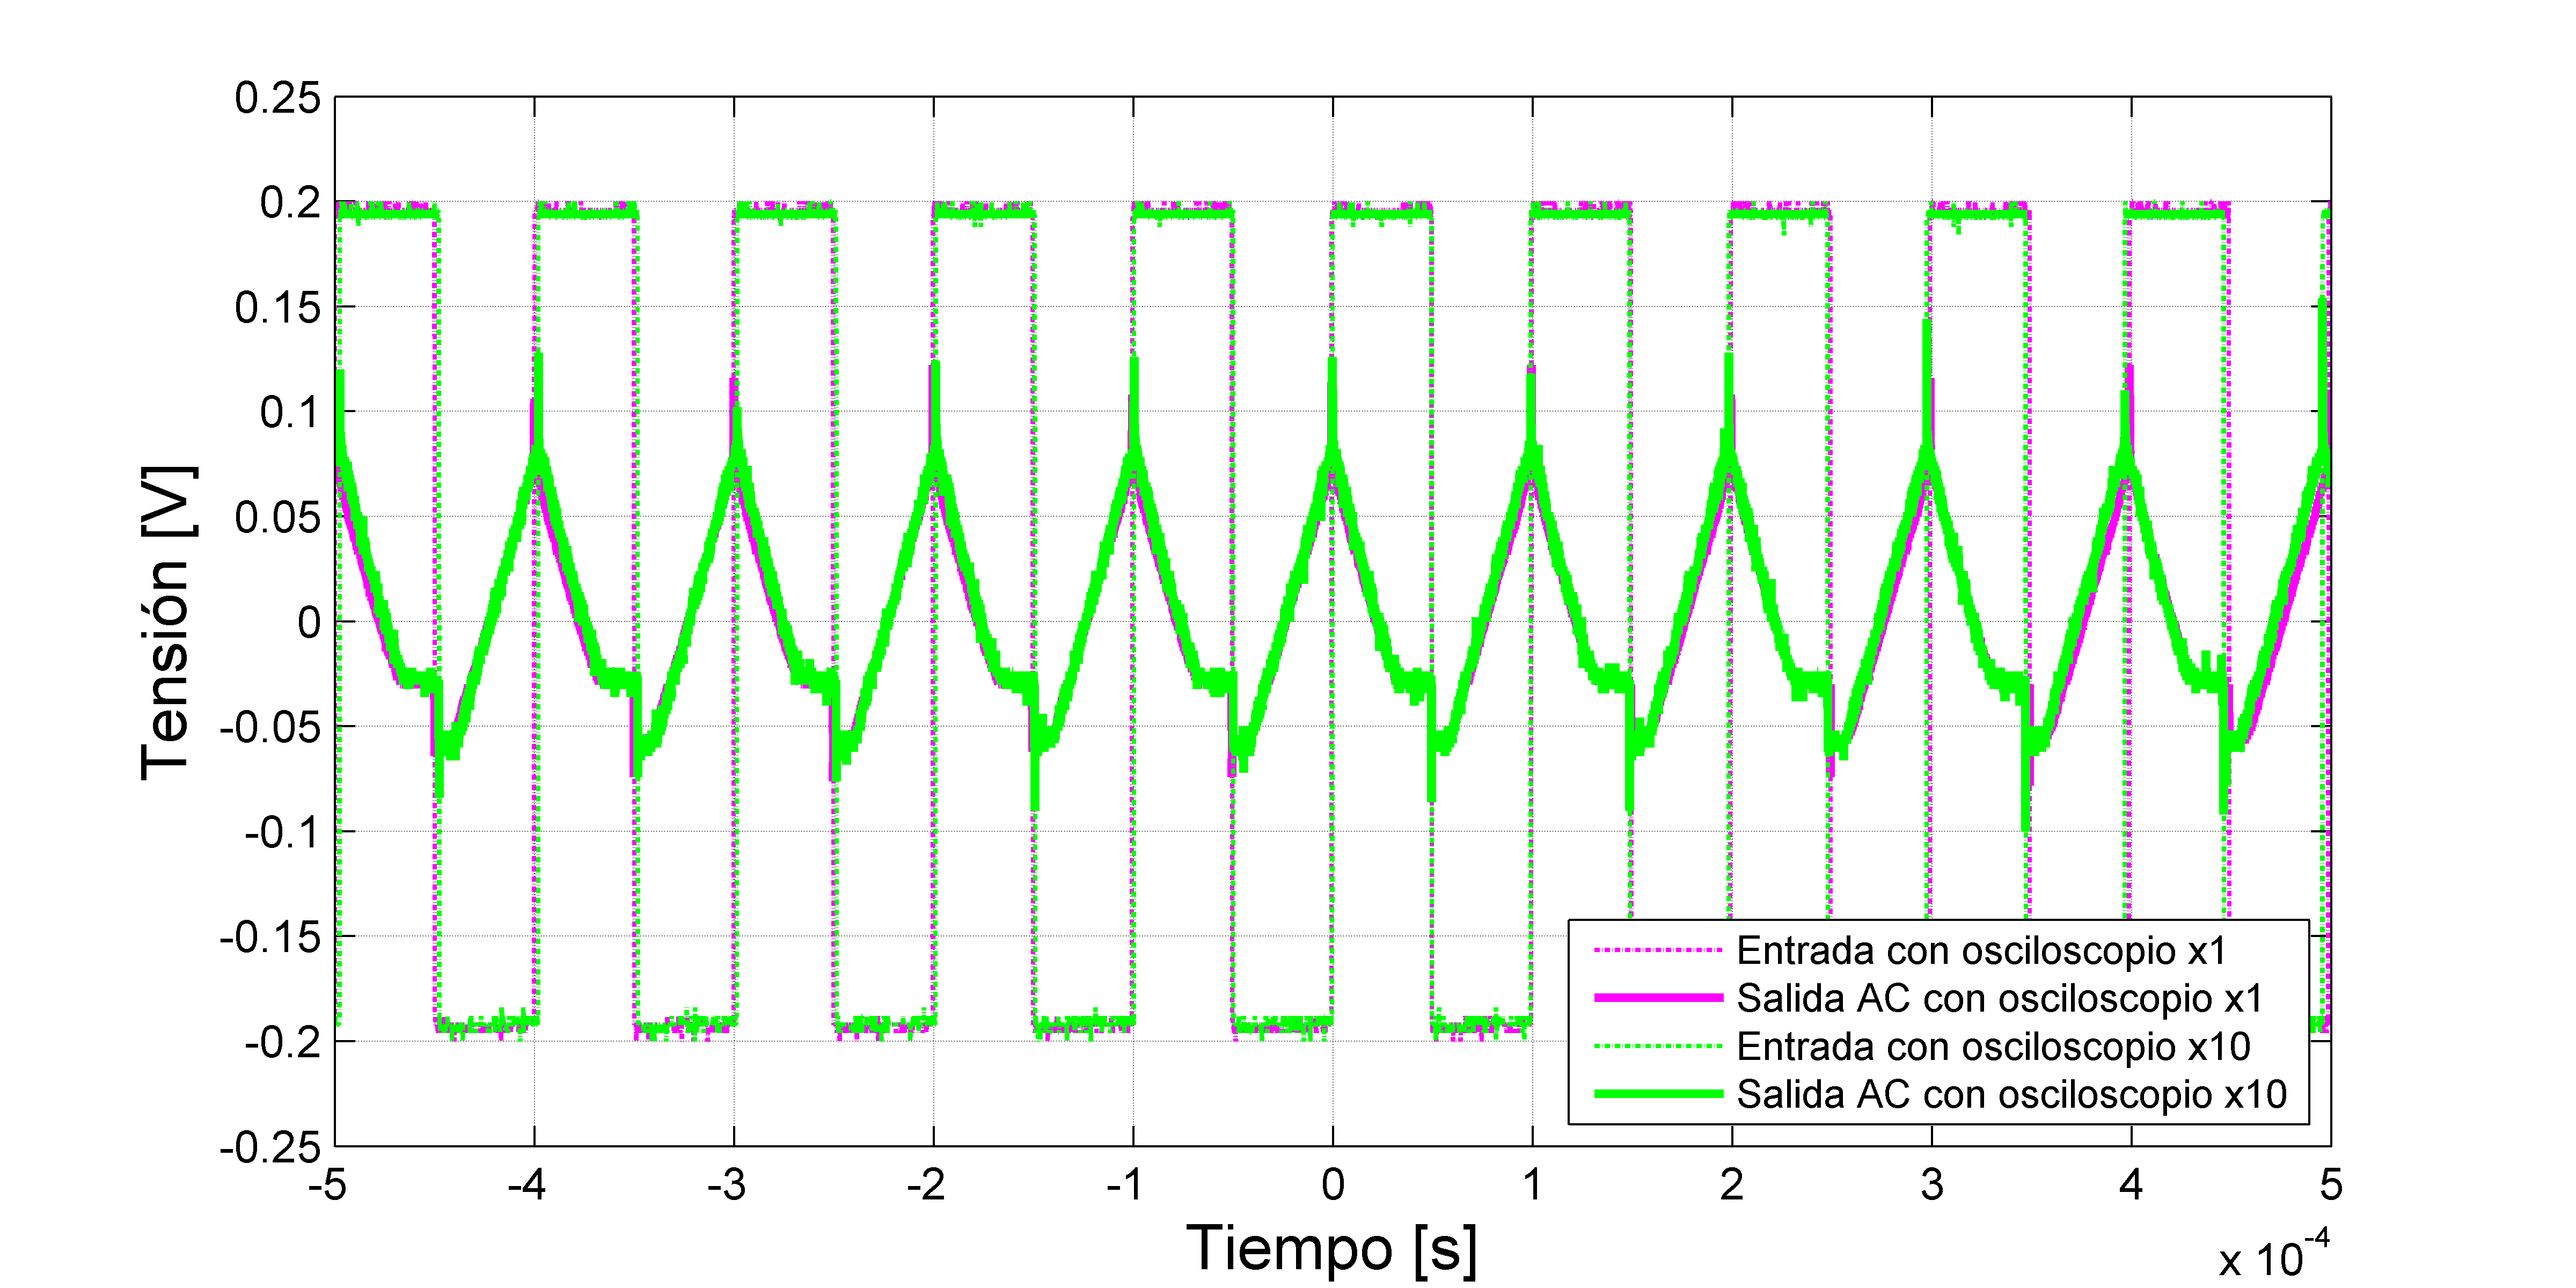
\includegraphics[width=1.1\textwidth]{gfx_22/INT1_M}
  \caption{Medición de la respuesta temporal del circuito integrador.}
  \label{m:int1}
\end{figure}

\begin{figure}[H]
  \centering
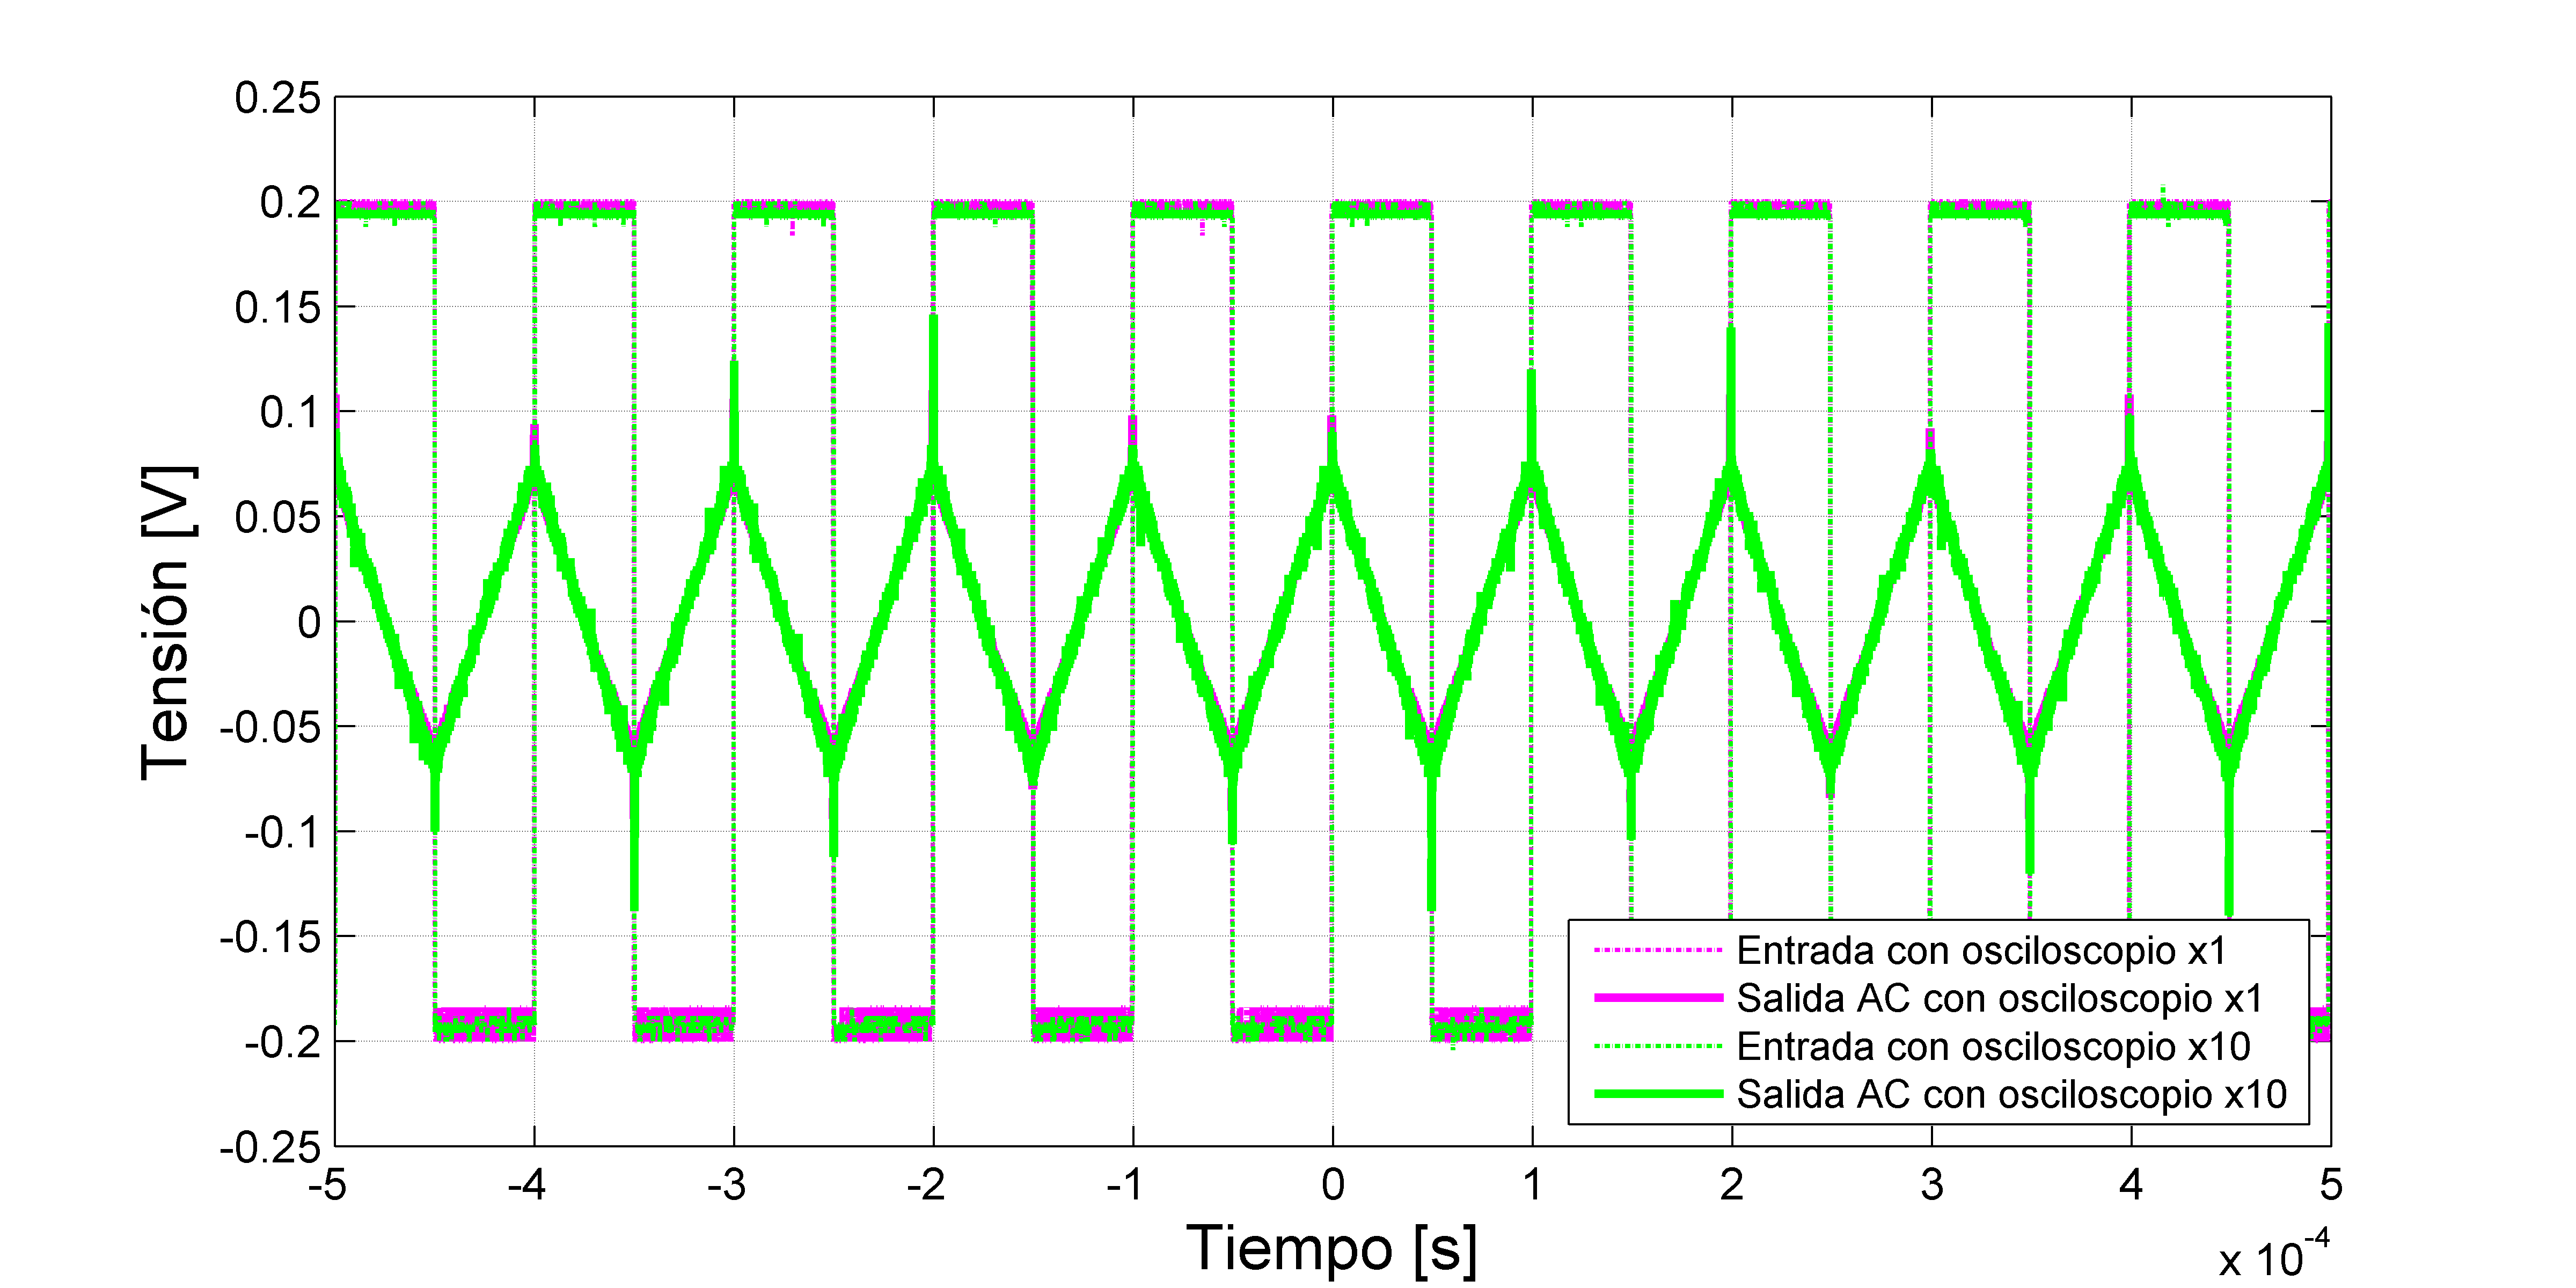
\includegraphics[width=1.1\textwidth]{gfx_22/INT2_M}
  \caption{Medición de la respuesta temporal del circuito integrador con control de ganancia.}
  \label{m:int2}
\end{figure}


\begin{figure}[H]
  \centering
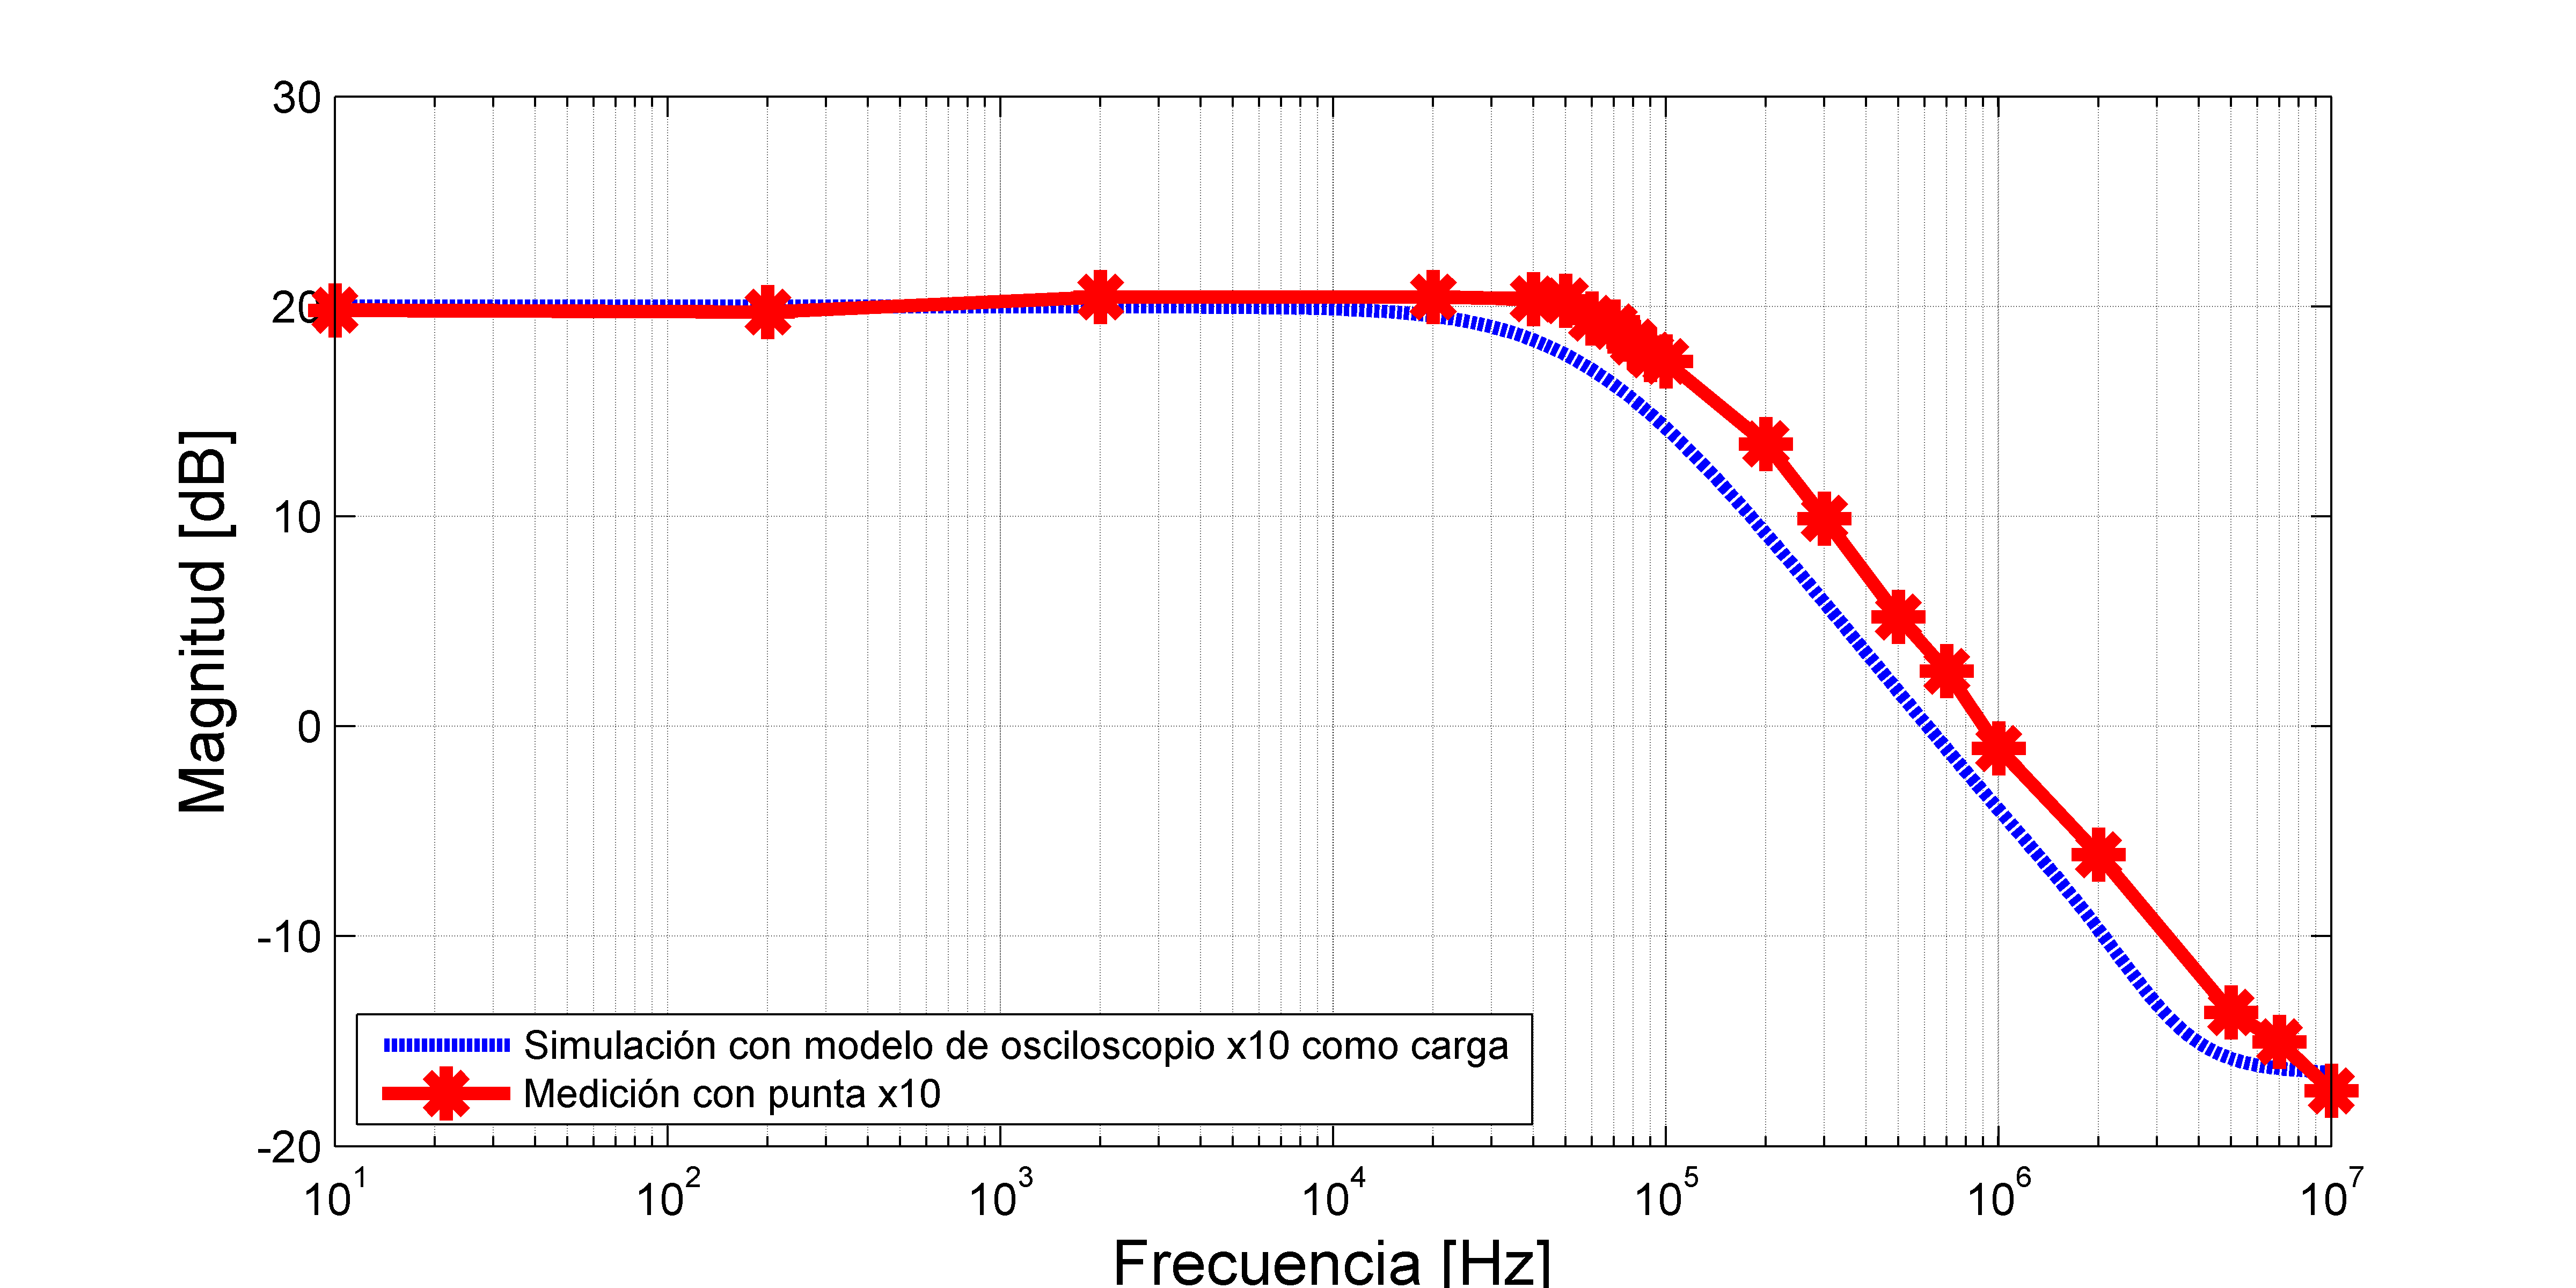
\includegraphics[width=1.1\textwidth]{gfx_22/INT2_MF}
  \caption{Medición de la respuesta en frecuencia del circuito integrador con control de ganancia medido con el osciloscopio en punta $10x$ y su comparación contra la simulación.}
  \label{mf:int2}
\end{figure}



\subsection{Circuito sumador}

La Figura \ref{circ:sum} muestra el esquemático de un circuito sumador, mientras que la Figura \ref{t:sum} representa la respuesta de la simulación tras introducirle a la entrada dos sinusoidales de amplitudes $20mV$ y $200mV$ a $1kHz$ en fase.

La respuesta a baja frecuencia de este circuito se rige por la ecuación:

\begin{equation}
v_o(t) = - 10.(v_a(t)+v_b(t))
\end{equation}


\begin{figure}[H]
  \centering
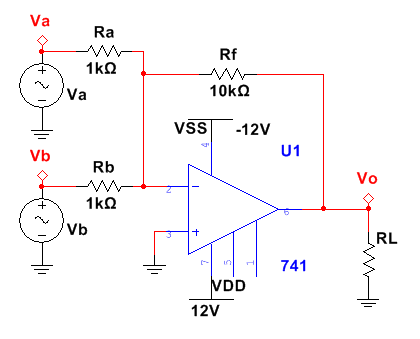
\includegraphics[width=.5\textwidth]{gfx/SUM_CIRC}
  \caption{Circuito sumador.}
  \label{circ:sum}
\end{figure}



\begin{figure}[H]
  \centering
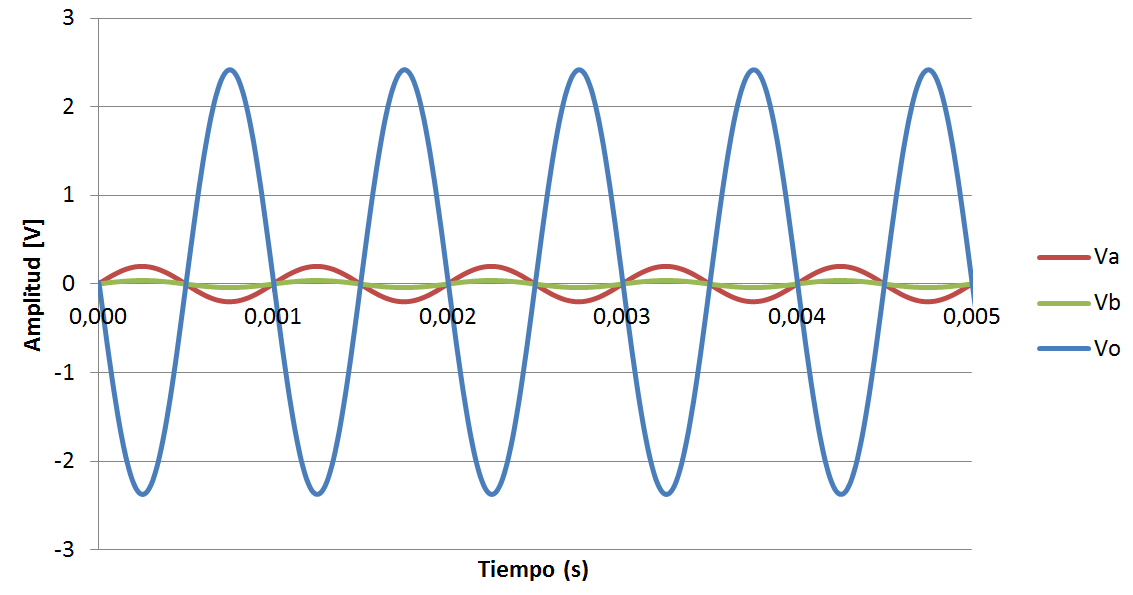
\includegraphics[width=.8\textwidth]{gfx/SUM1}
  \caption{Simulación temporal del circuito sumador.}
  \label{t:sum}
\end{figure}



\subsection{Circuito diferenciador}

El esquemático de este circuito es el presentado en la Figura \ref{circ:diff}, mientras que las ecuaciones paramétricas del sistema considerando componentes ideales son:

\begin{equation*}
C.\frac{dv_1(t)}{dt} = -\frac{0V-v_O(t)}{R}
\end{equation*}


\begin{equation}
v_O(t) = -R.C.\frac{dv_1(t)}{dt} = - 10^{-5}.\frac{dv_1(t)}{dt}
\end{equation}


\begin{figure}[H]
  \centering
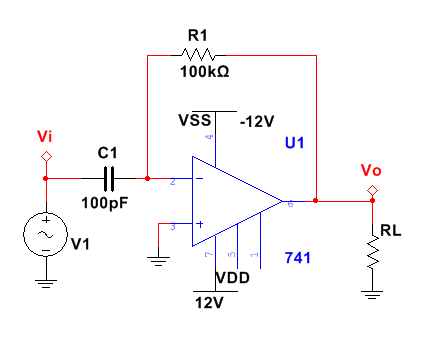
\includegraphics[width=.5\textwidth]{gfx/DIFF}
  \caption{Circuito diferenciador.}
  \label{circ:diff}
\end{figure}

\begin{figure}[H]
  \centering
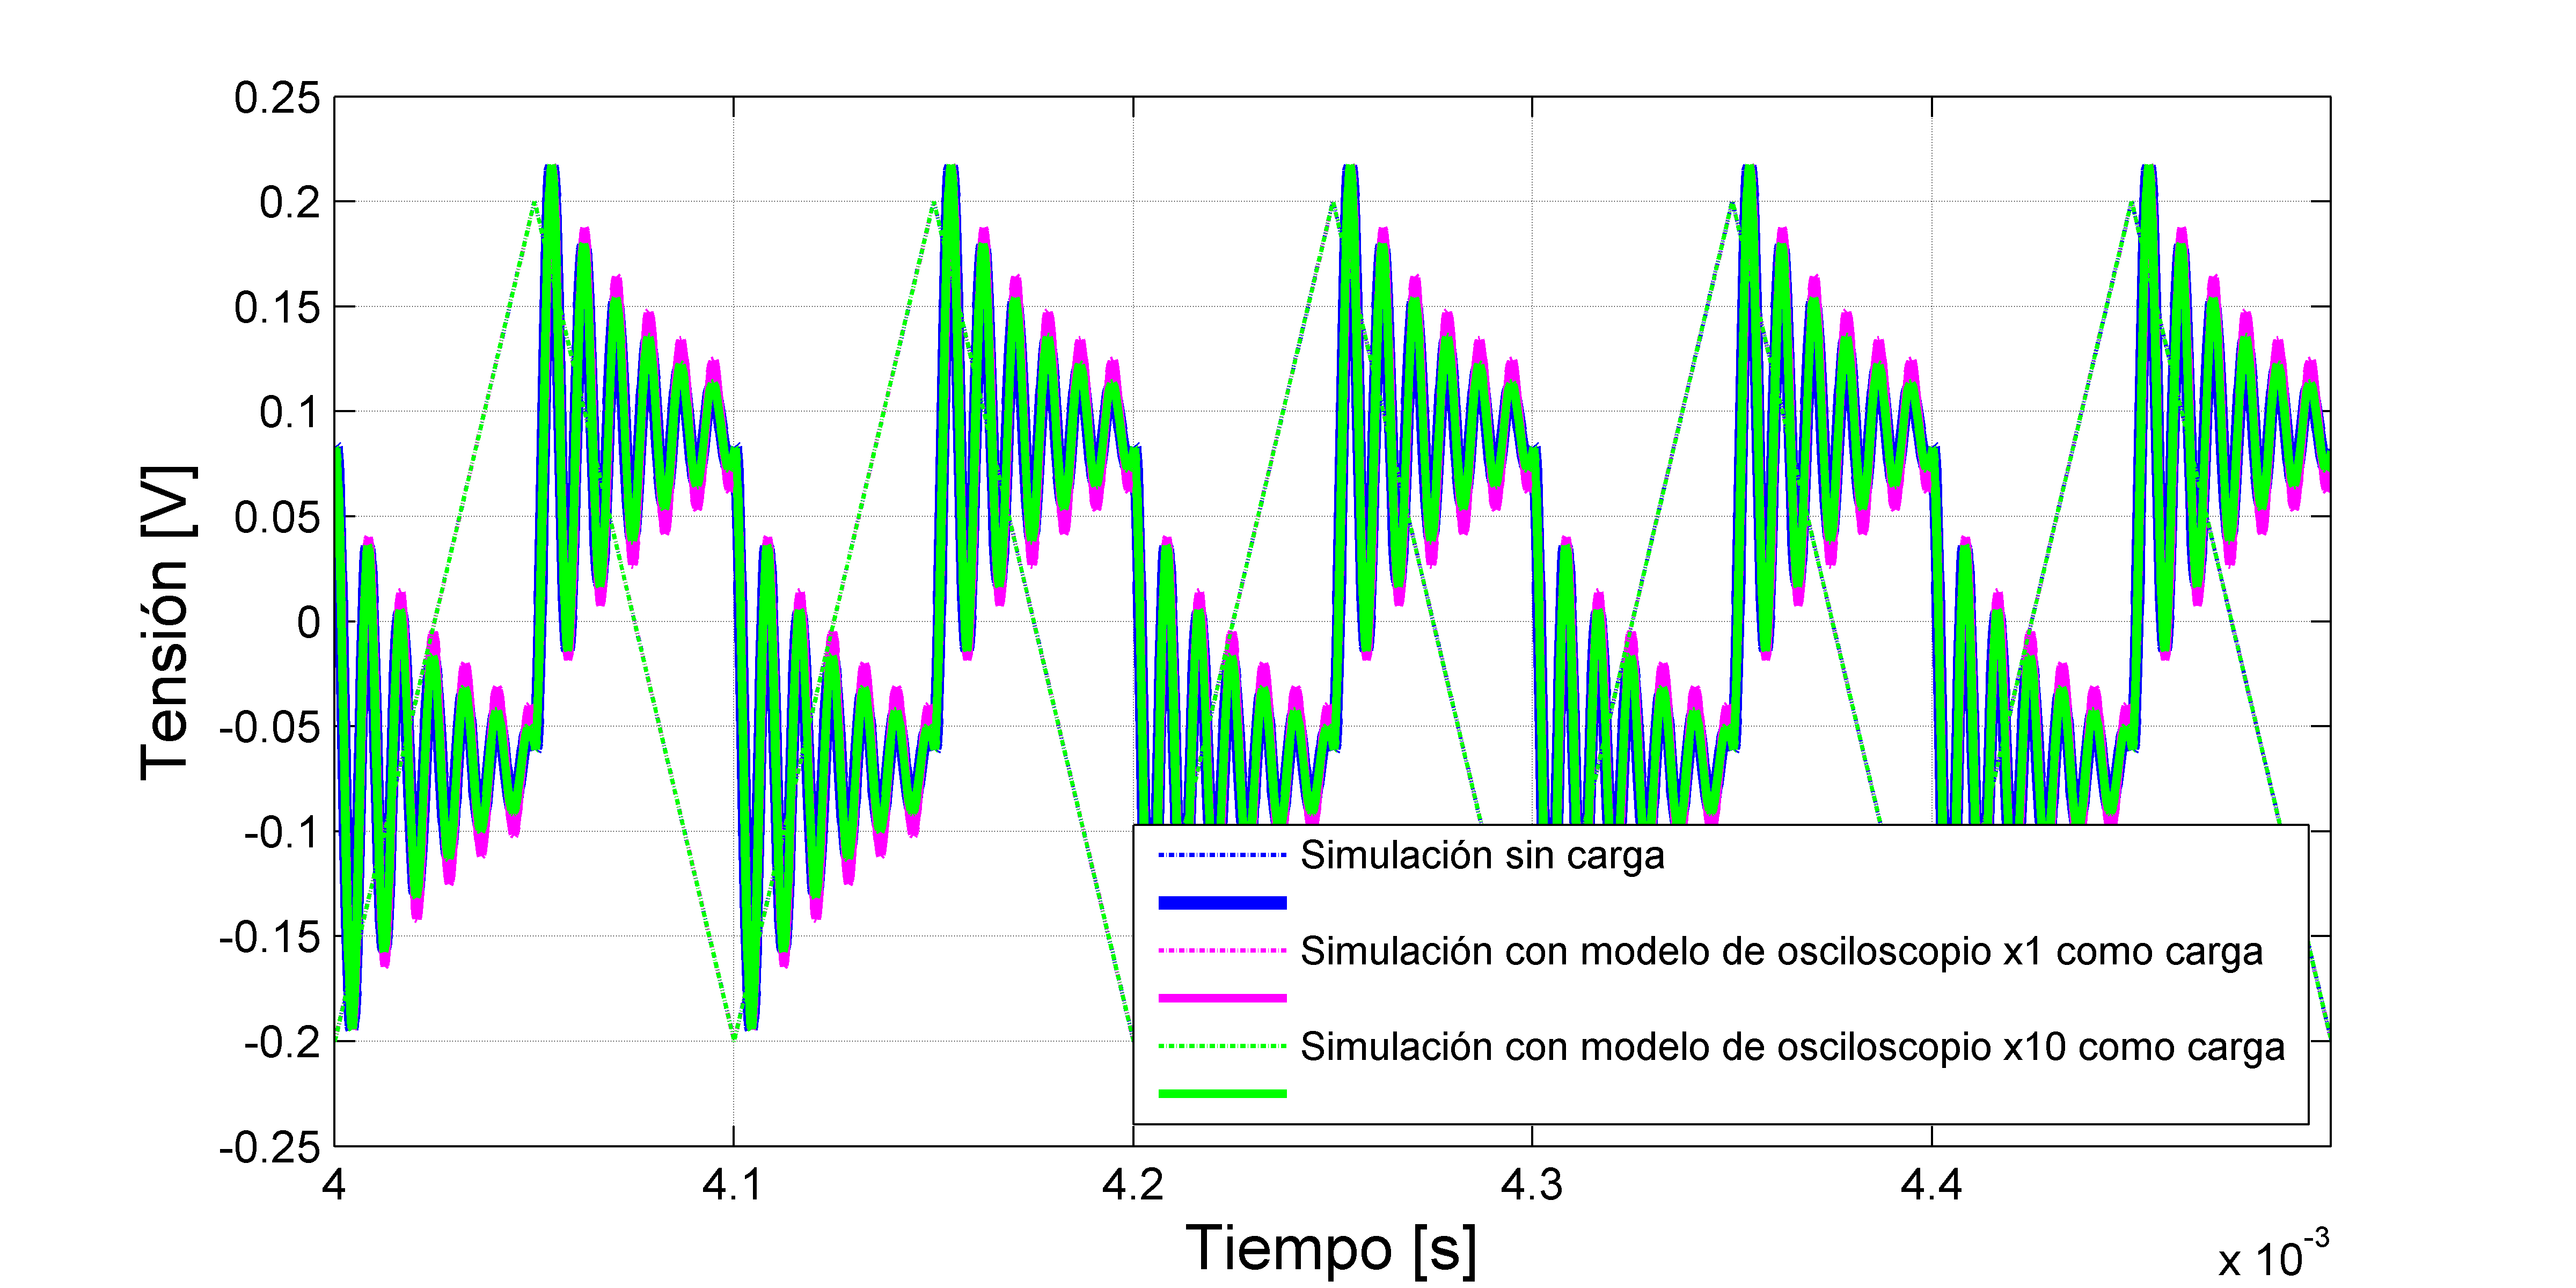
\includegraphics[width=1.1\textwidth]{gfx_22/DIFF_T}
  \caption{Respuesta del circuito diferenciador ante una señal triangular de $200mV$ con período de $100us$.}
  \label{t:diff}
\end{figure}


\noindent$\blacktriangle$\textbf{ ¿Qué problemas se encontraron al realizar la medición? Utilizar puntas directa y compensada.}

Este circuito no realizó la operación matemática de derivación de la señal triangular para generar una señal cuadrada.

De la resolución analítica se extrae que el circuito solo posee un cero a $0Hz$, y su amplificación en continua es $-10^{-5}$. Lo presentado en esta respuesta es la falta de compensación de amplificación a altas frecuencias. Es decir que el circuito es inestable a altas frecuencias.

Al ser la señal triangular compuesta por los infinitos armónicos múltiplos impares de la frecuencia fundamental, a la salida se ven estas componentes amplificadas.

Para compensar este problema (como en el integrador), se puede colocar una resistencia en serie al capacitor.


\begin{figure}[H]
  \centering
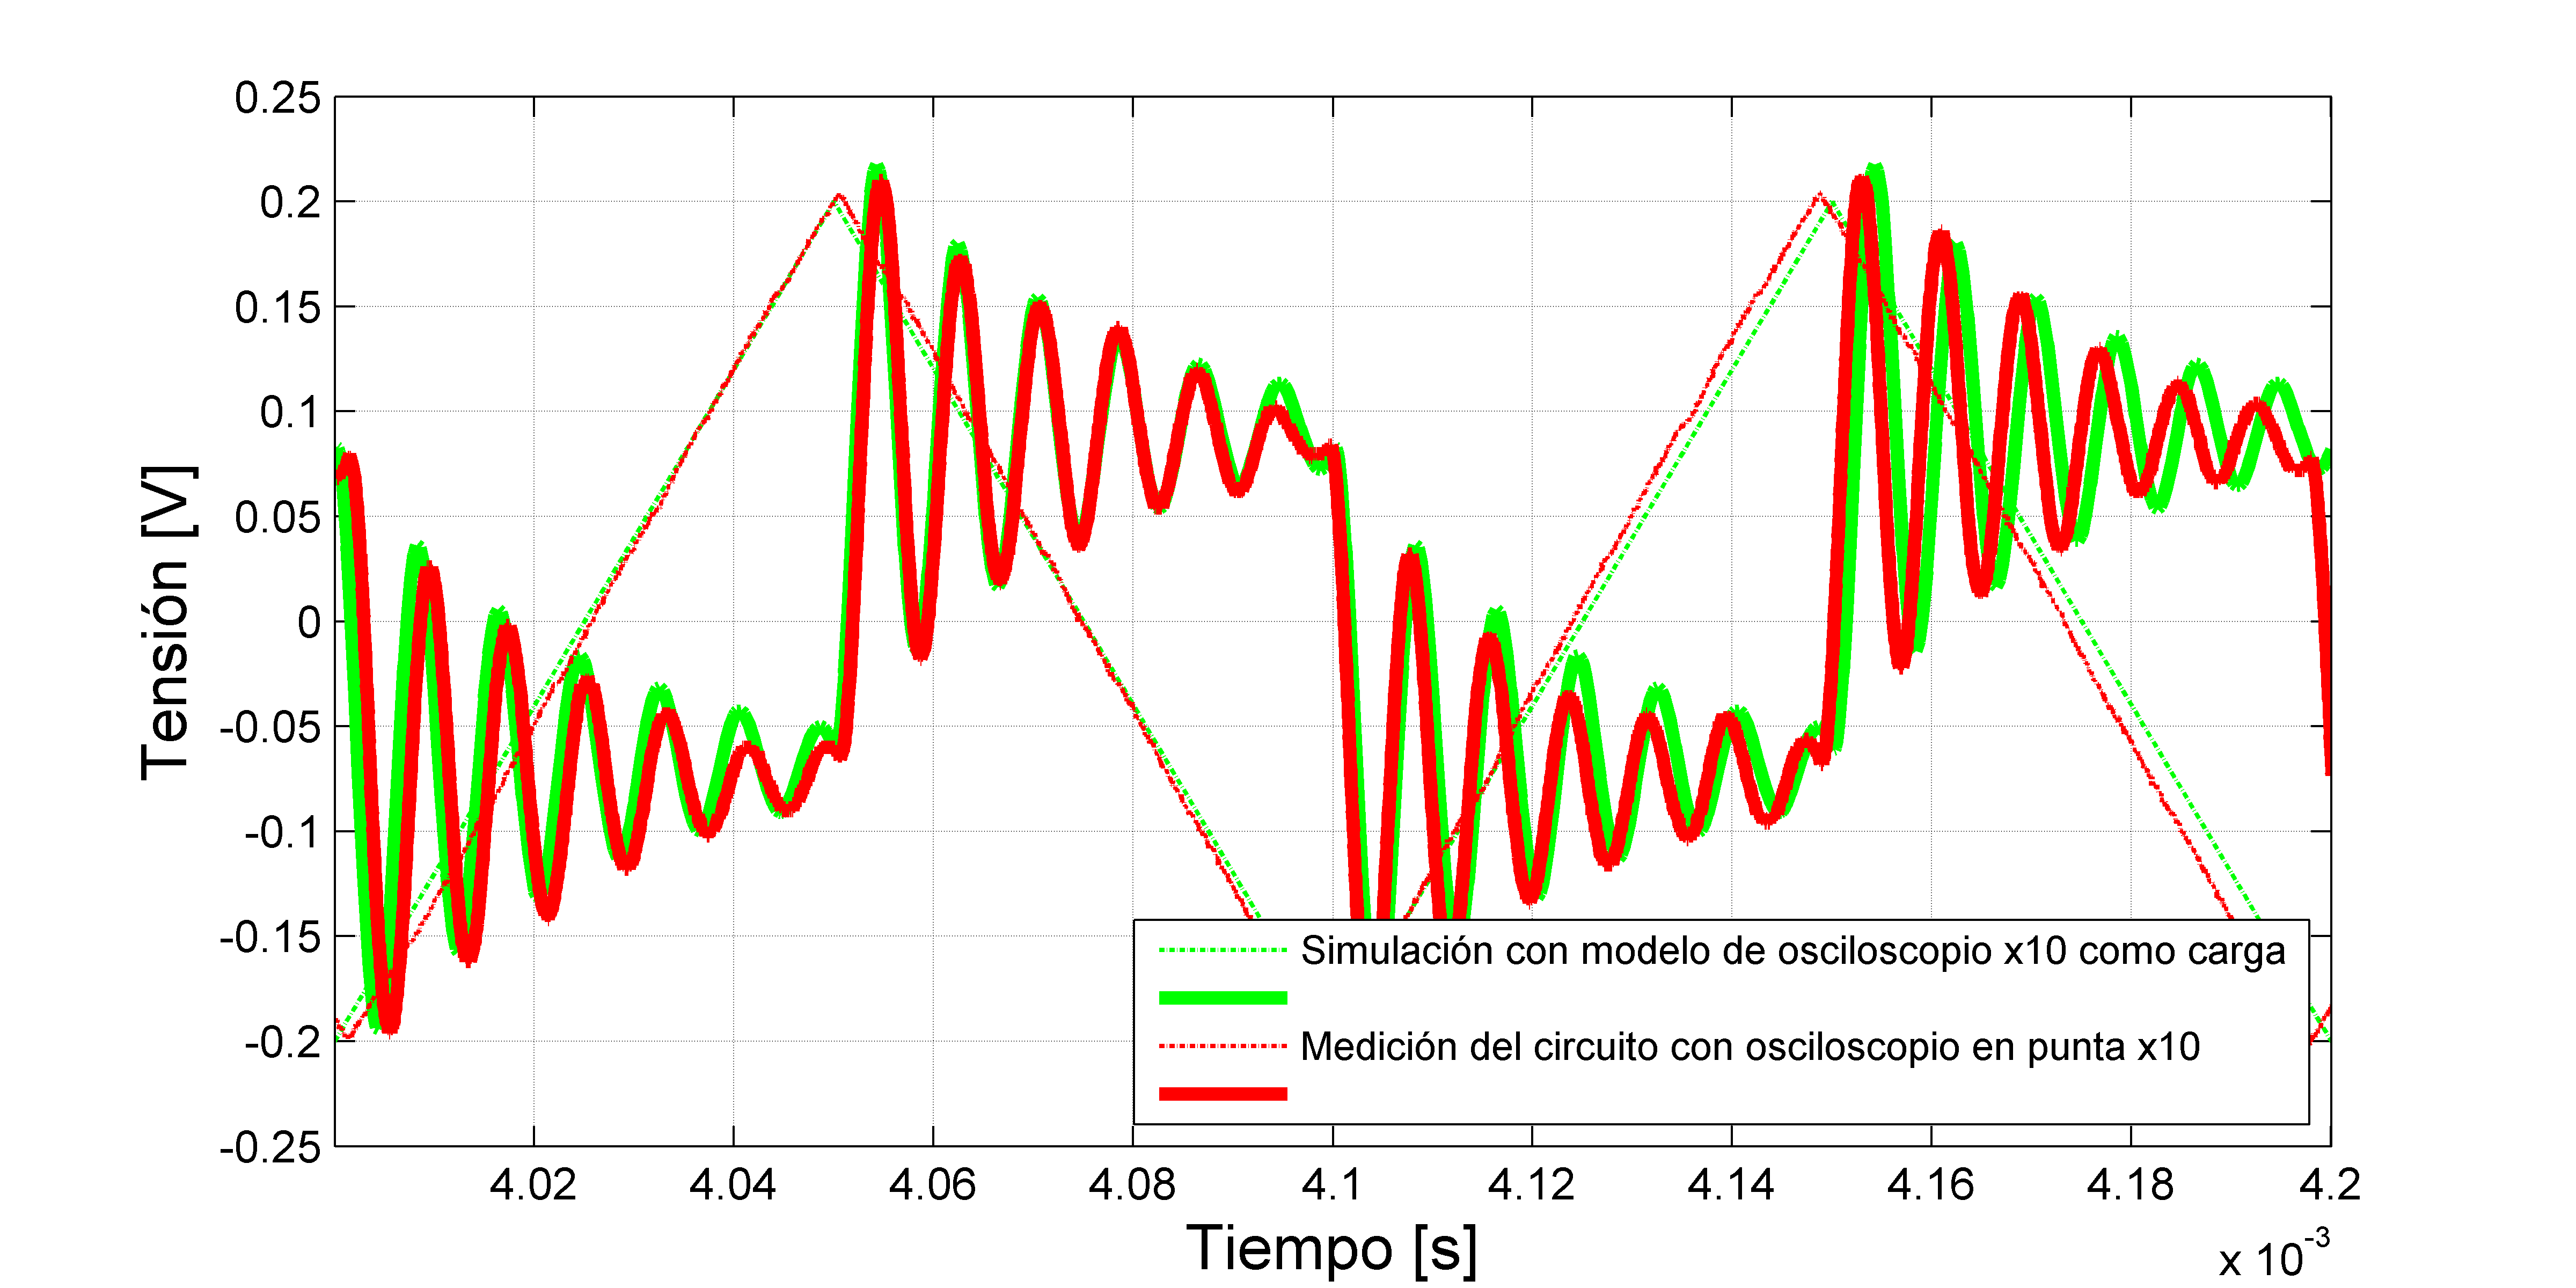
\includegraphics[width=1.1\textwidth]{gfx_22/DIFF_M}
  \caption{Comparación entre la simulación y la medición de la respuesta del circuito diferenciador.}
  \label{m:diff}
\end{figure}



\subsection{Amplificador logarítmico}

\begin{figure}[H]
  \centering
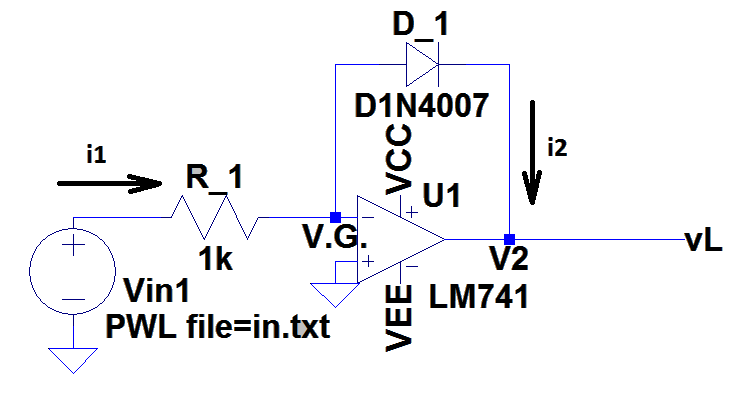
\includegraphics[width=.5\textwidth]{gfx_22/circ_log}
  \caption{Circuito amplificador logarítmico.)}
  \label{circ:log}
\end{figure}


El siguiente circuito a analizar es el de la Figura \ref{circ:log}. Se procede a realizar el análisis circuital con los modelos ideales ya discutidos:

\begin{equation}
\frac{v_{in}(t)-V_{irtual}G_{round}}{R_1}= I_s.e^{\frac{V_{irtual}G_{round}-v_L(t)}{V_T}}
\end{equation}

\begin{equation}
v_L(t) = V_T.ln(\frac{R_1.I_S}{v_{in}}) = 25mV.ln(\frac{10uV}{v_{in}(t)})
\end{equation}

Se identifica una característica logarítmica en cuanto a la respuesta, la cual se corresponde a un sistema alineal.

Los gráficos comparativos entre la simulación y la medición de la respuesta ante señales de $12mV$ a frecuencias $1kHz$, $3kHz$ y $10kHz$ se muestran en las Figuras \ref{v:log1}, \ref{v:log3} y \ref{v:log10} respectivamente.

La dispersión de las muestras tomadas del osciloscopio se da debido al ruido de las mediciones sobre la tensión de la señal de $12mV_p$ a la entrada. Esto puede ser visto en la Figura \ref{t:log}, donde se muestra la respuesta alterna ante la señal diente de sierra de $10kHz$.


\begin{figure}[H]
  \centering
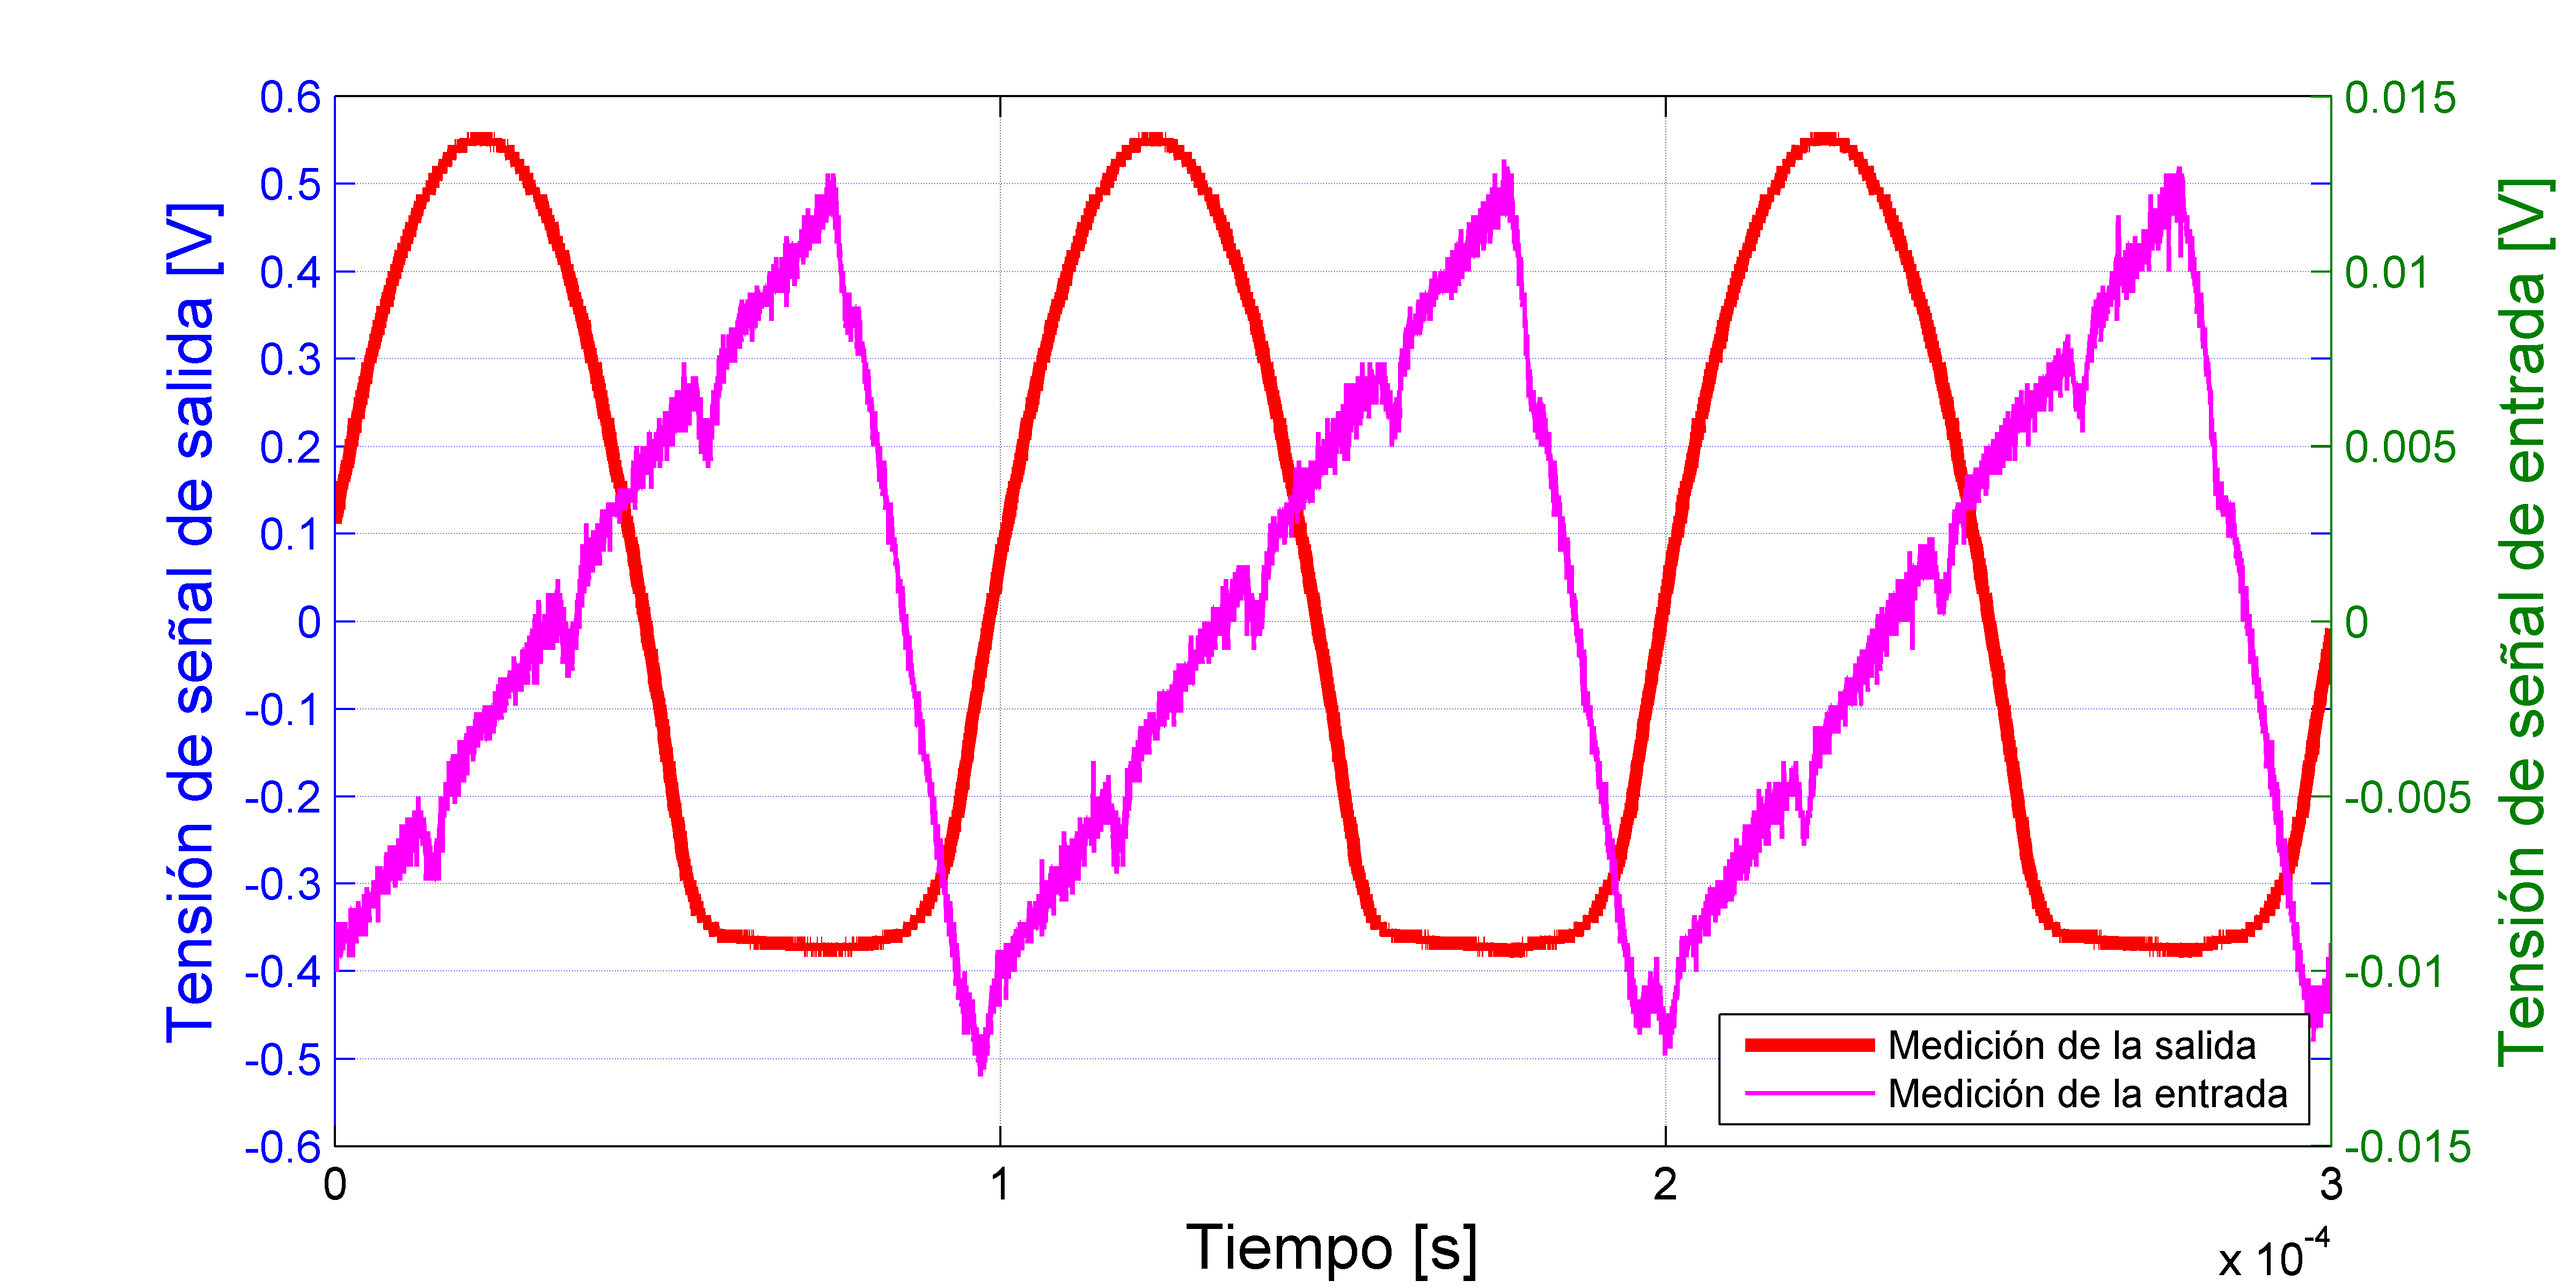
\includegraphics[width=.8\textwidth]{gfx_22/LOG_t}
  \caption{Medición de la respuesta alterna del circuito logarítmico ante una señal diente de sierra de $10kHz$.}
  \label{t:log}
\end{figure}


\begin{figure}[H]
  \centering
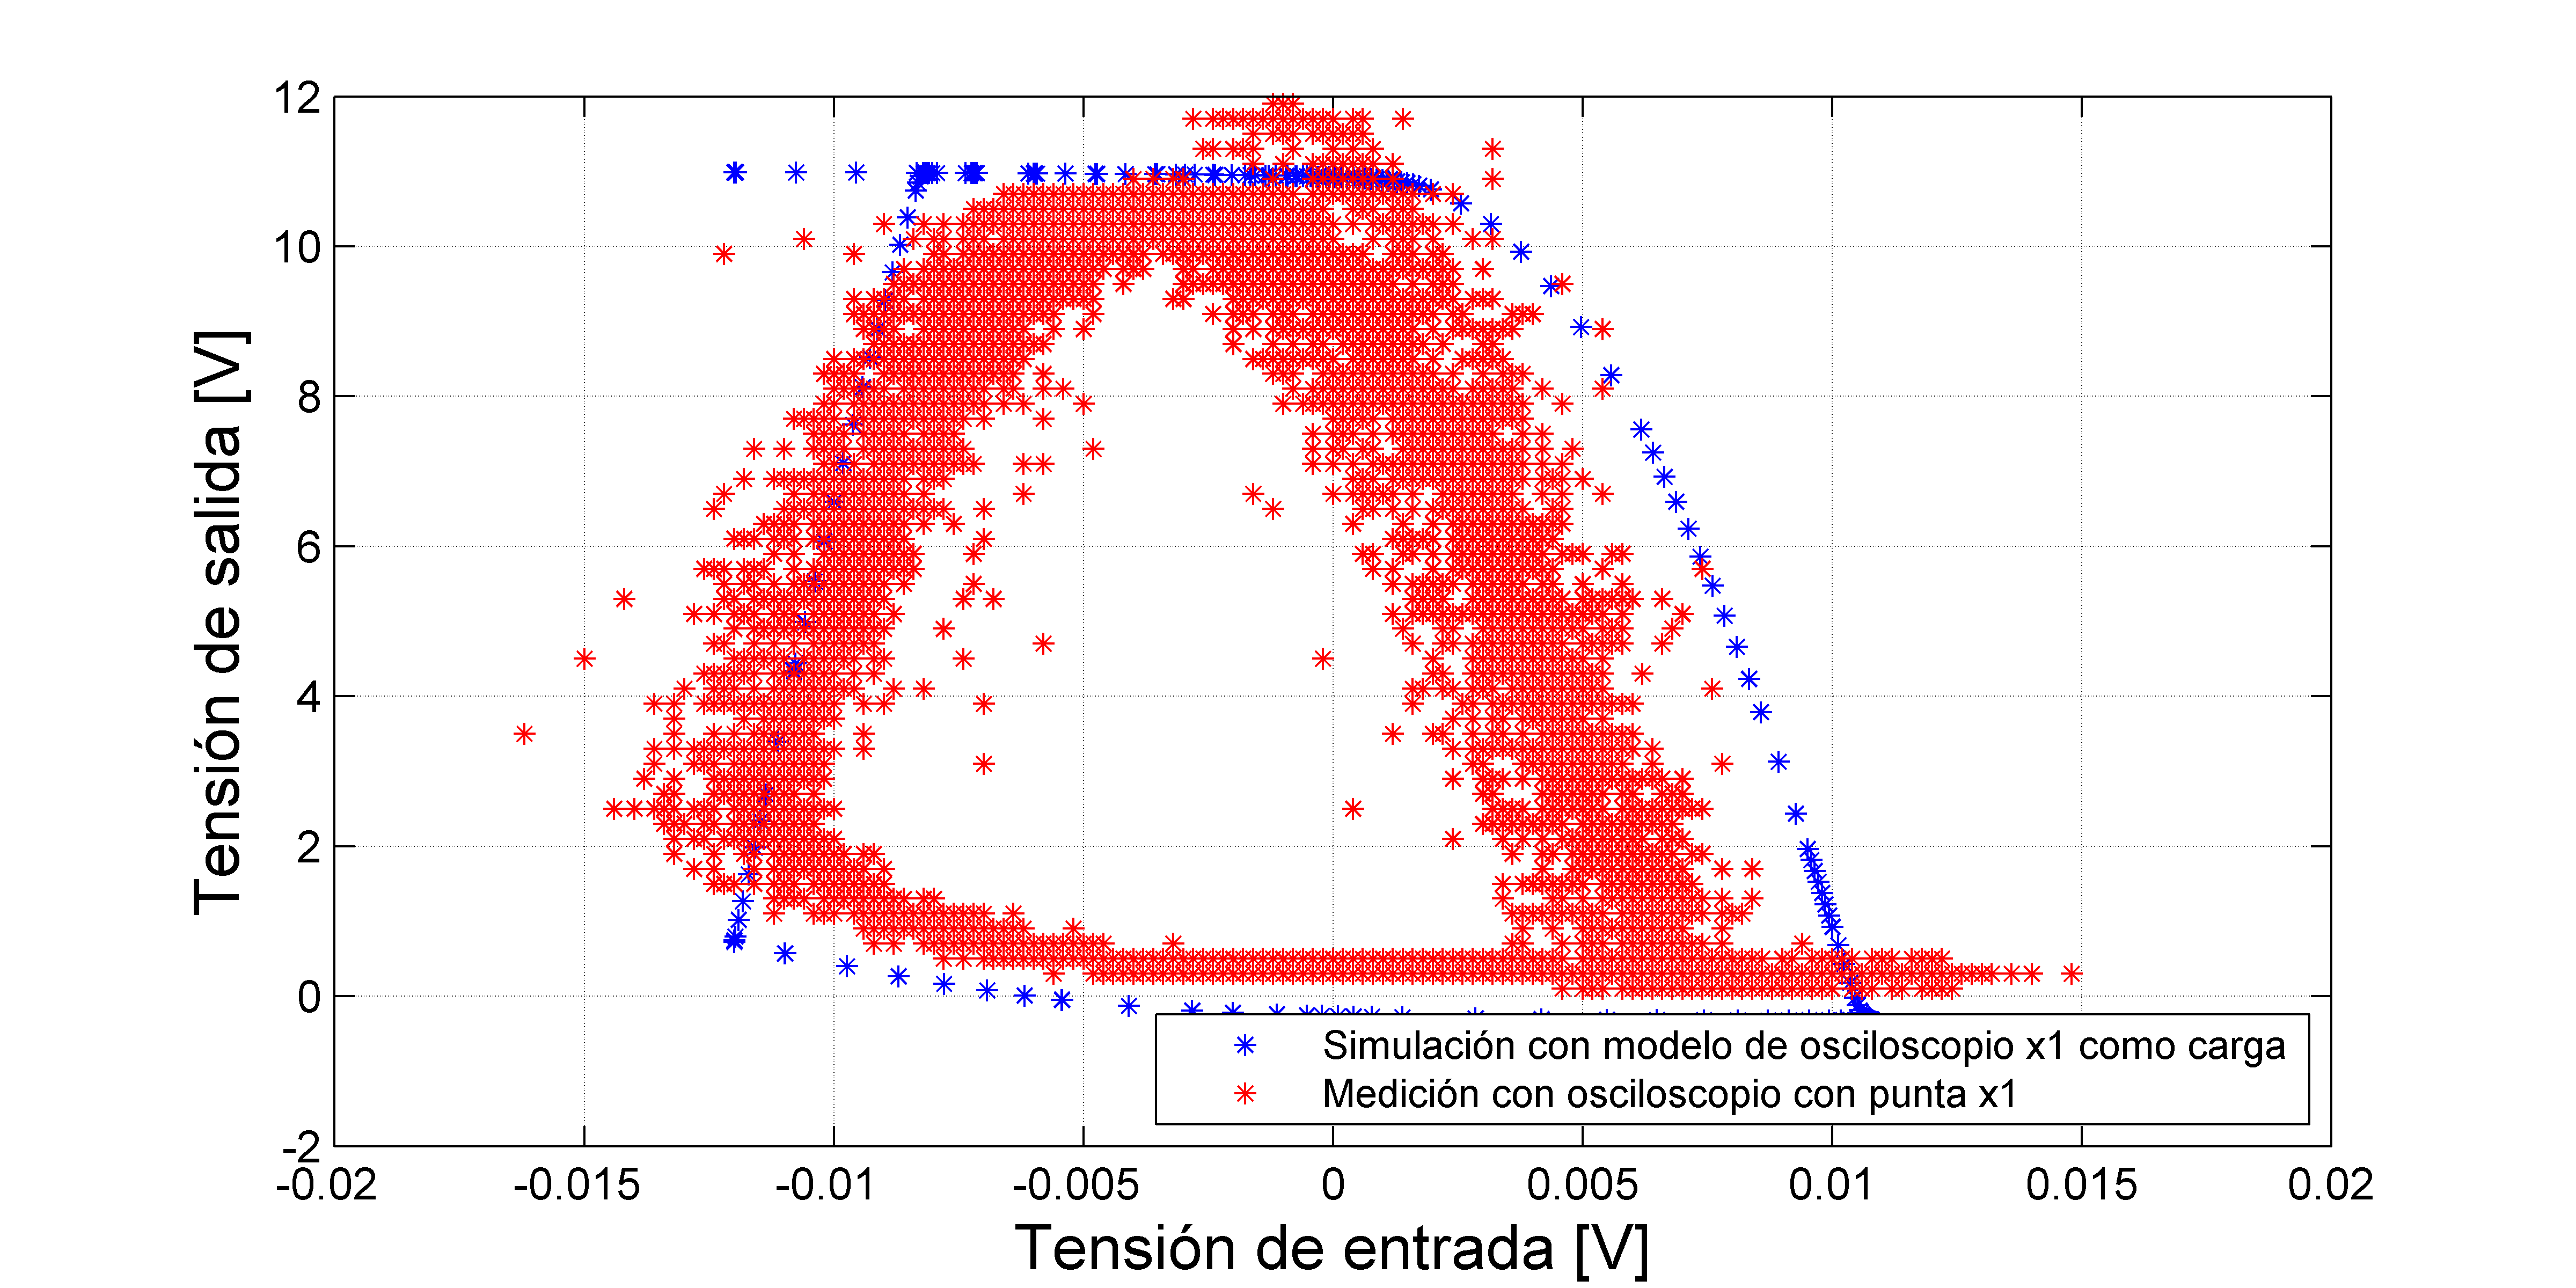
\includegraphics[width=1.1\textwidth]{gfx_22/LOG_1}
  \caption{Comparación entre simulación y medición de la relación entre la señal de entrada y salida para una frecuencia de $1kHz$.}
  \label{v:log1}
\end{figure}


\begin{figure}[H]
  \centering
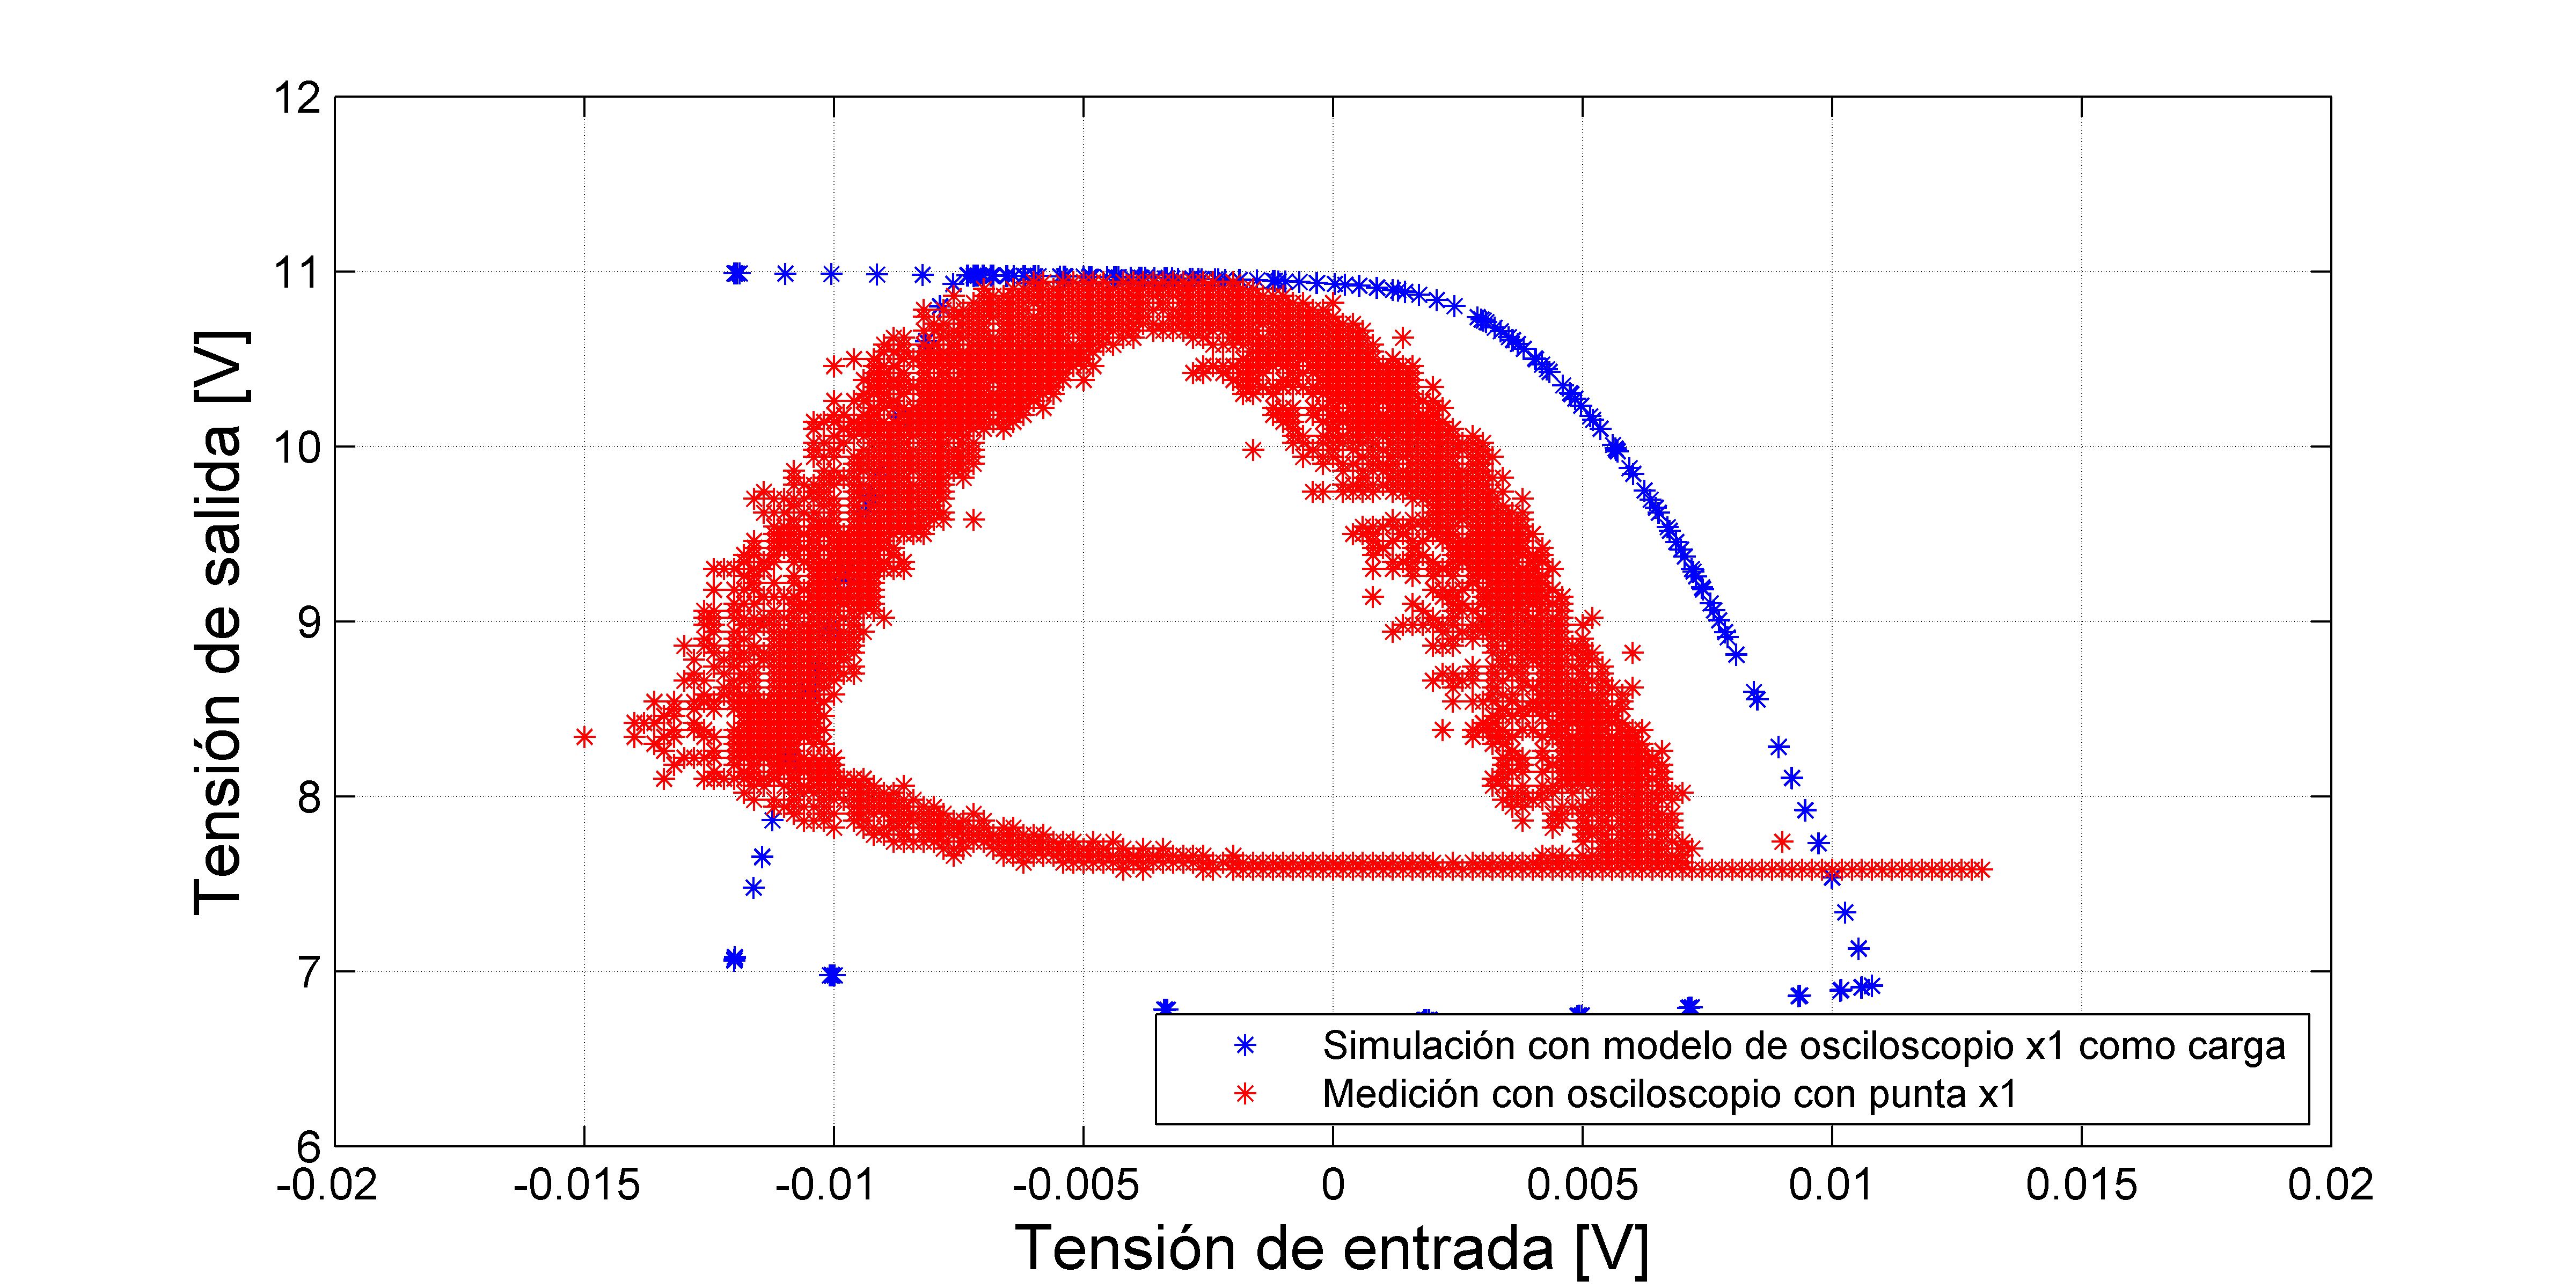
\includegraphics[width=1.1\textwidth]{gfx_22/LOG_3}
  \caption{Comparación entre simulación y medición de la relación entre la señal de entrada y salida para una frecuencia de $3kHz$.}
  \label{v:log3}
\end{figure}



\begin{figure}[H]
  \centering
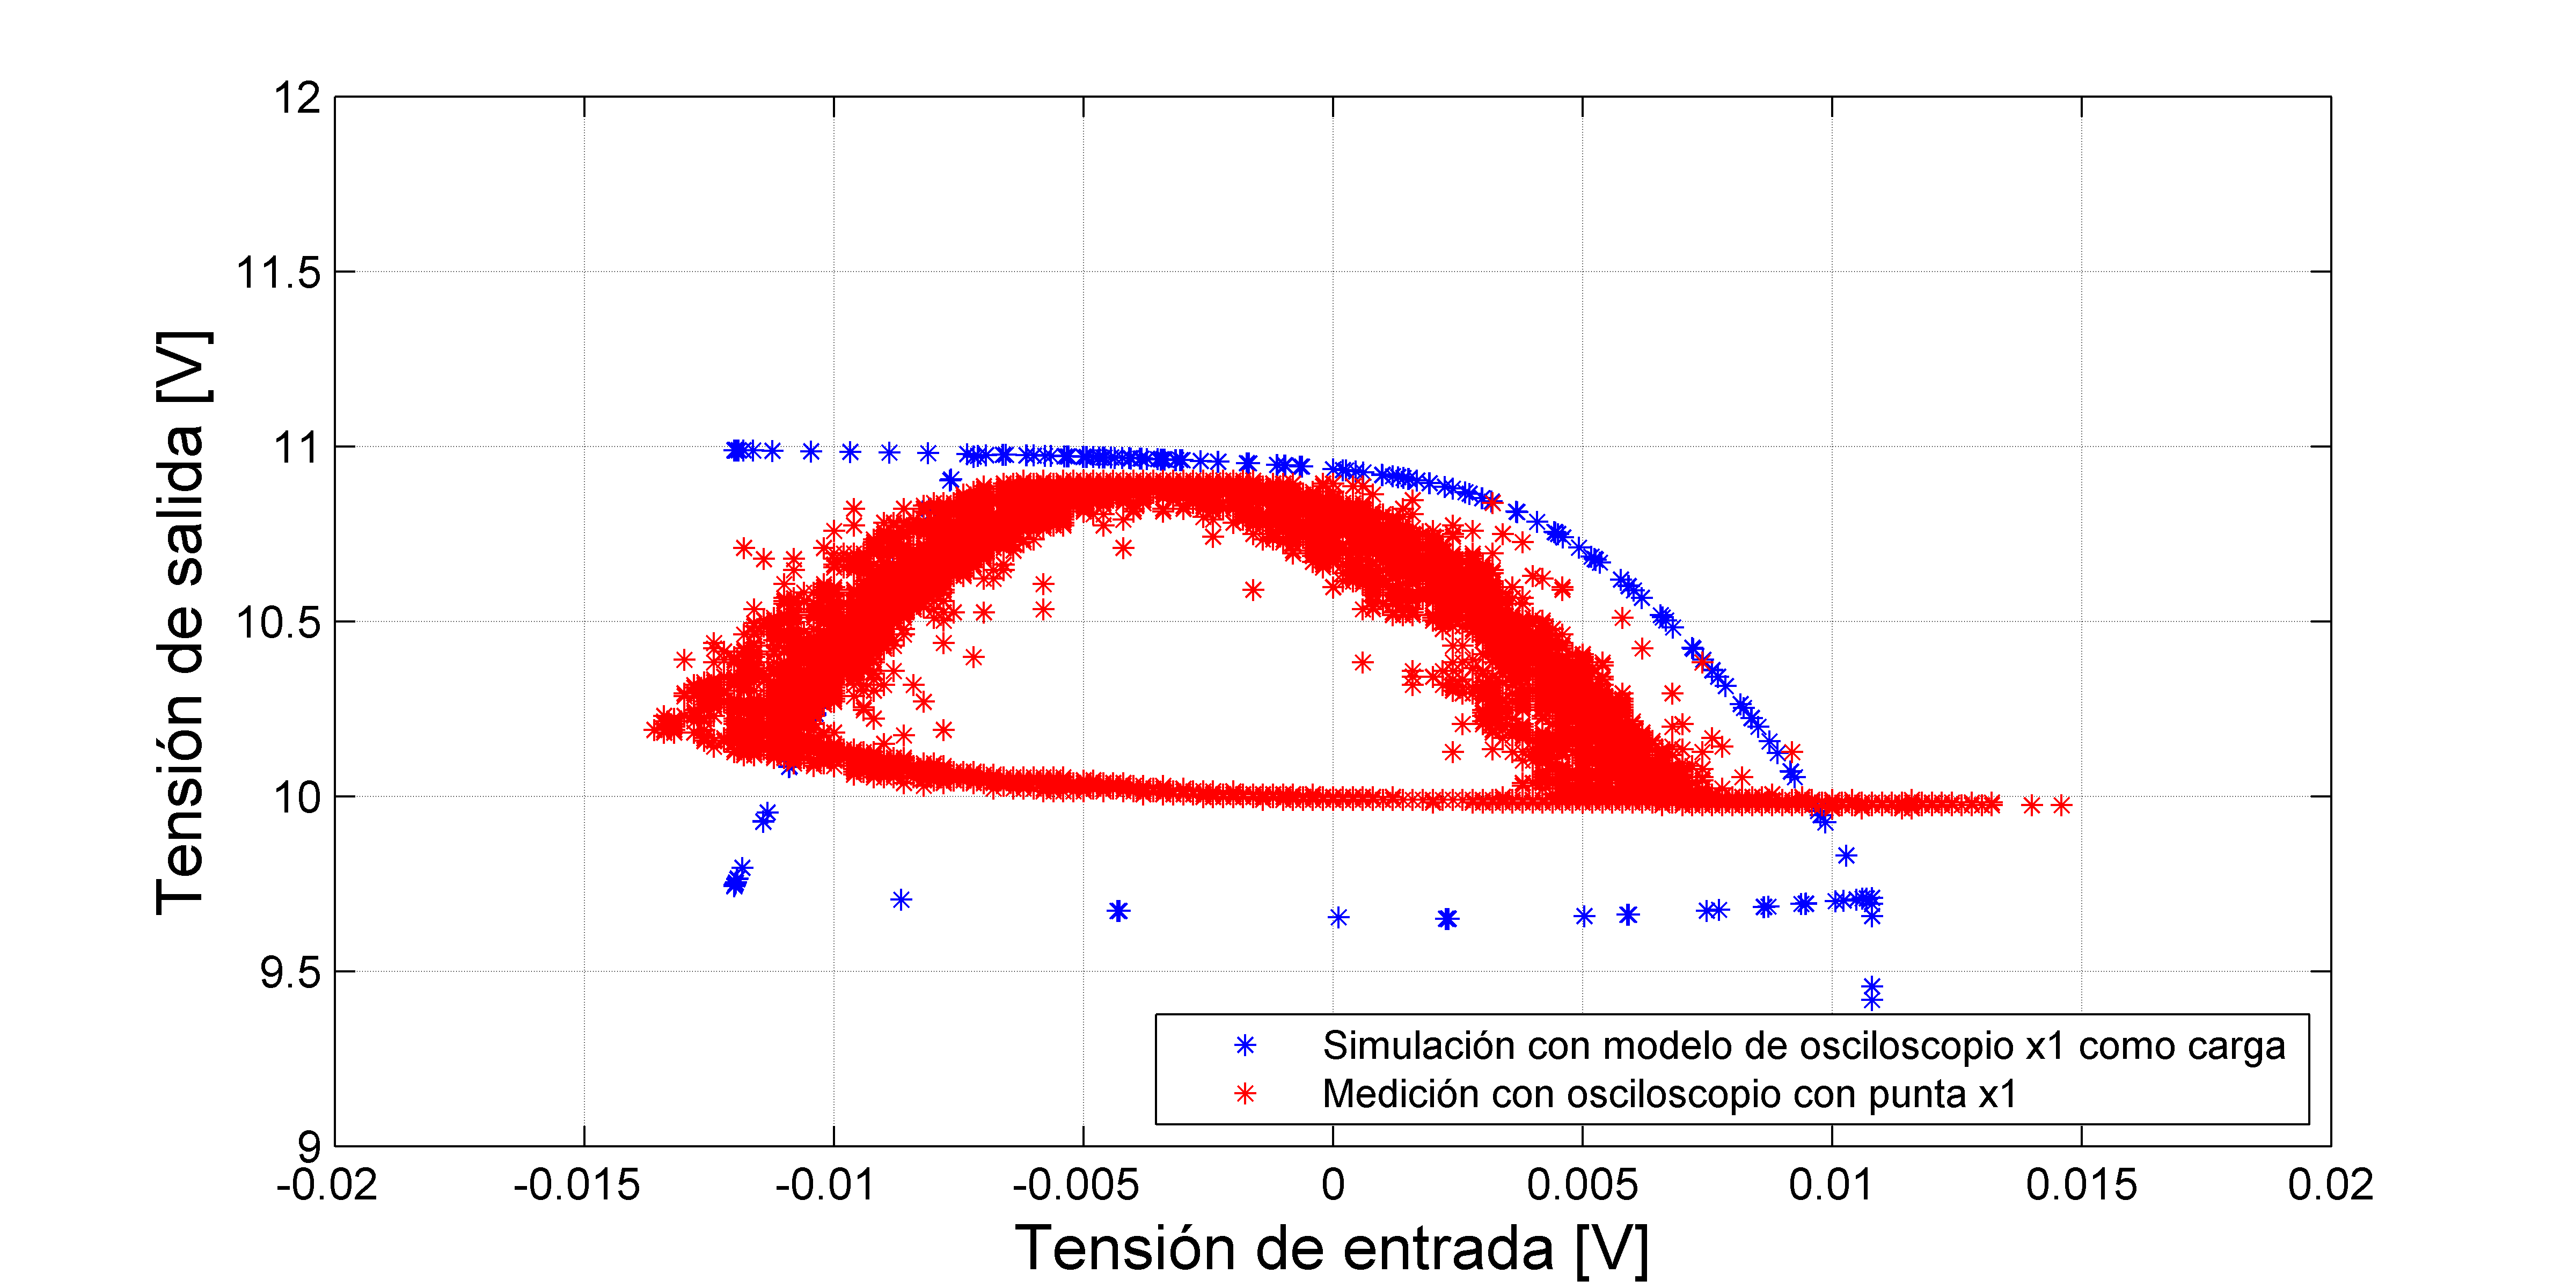
\includegraphics[width=1.1\textwidth]{gfx_22/LOG_10}
  \caption{Comparación entre simulación y medición de la relación entre la señal de entrada y salida para una frecuencia de $10kHz$.}
  \label{v:log10}
\end{figure}

Mientras que en los circuitos anteriores se contaba con sistemas lineales (siempre y cuando se trabaje sin saturar señales), aquí es posible apreciar la curva exponencial que introduce el diodo al circuito.


\subsubsection{Aplicaciones de la etapa}

\begin{itemize}
\item Medir una magnitud muy grande, tal que se haga énfasis en la zona de menor amplitud.


\item Se puede medir la respuesta de un diodo ante una rampa y verificar si tras pasar por el filtro, ésta es lineal.

\item Tras una serie de cálculos y ajustes de componentes, es posible transformar un nivel tensión a decibeles en la salida, de modo que la función de transferencia sea $20.log(\frac{v_1}{v_{ref}})$

\item Con unos ligeros retoques al circuito, es factible obtener un sistema que reproduce la exponencial de la entrada, lo que permitiría identificar los picos de señales de muy baja magnitud. Esta etapa podría ser implementada, por ejemplo, para la detección de pulsos de baja amplitud en una señal ruidosa.
\end{itemize}








\clearpage
\section{Rectificadores}
\label{sec:rect}
\subsection{Rectificador de media onda simple}
\begin{figure}[H]
  \centering
      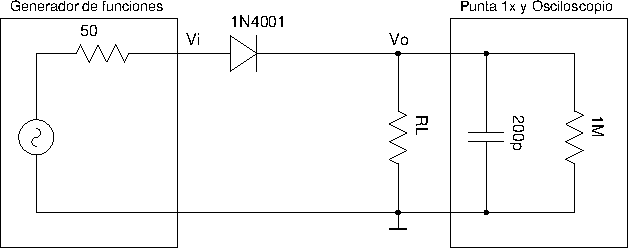
\includegraphics[width=0.8\textwidth]{gfxsantiago/FIG_CIRC_Rectificador_Simple_A.pdf}
  \caption{Circuito correspondiente al rectificador simple junto con el banco de medición utilizado y los equivalentes Thevenin de los instrumentos que fueron considerados para las simulaciones.}
  \label{fig:circ_3A}
\end{figure}
En esta parte del trabajo realizaremos mediciones relacionadas con el circuito que se muestra en la Figura \ref{fig:circ_3A}, el cual se denomina rectificador de media onda. El diodo utilizado es el 1N4001 y el resistor será de $R_{L} = 10 k\Omega$. El banco de medición correspondiente se muestra en la figura ya mencionada, el cual consta del circuito en cuestión excitado por una señal sinusoidal de $50Hz$ y amplitud $5V$ proveniente de un generador de funciones y los equivalentes de Thevenin correspondientes al generador de funciones y a la punta 1x que se conecta al osciloscopio.\\

\begin{figure}[H]
  \centering
      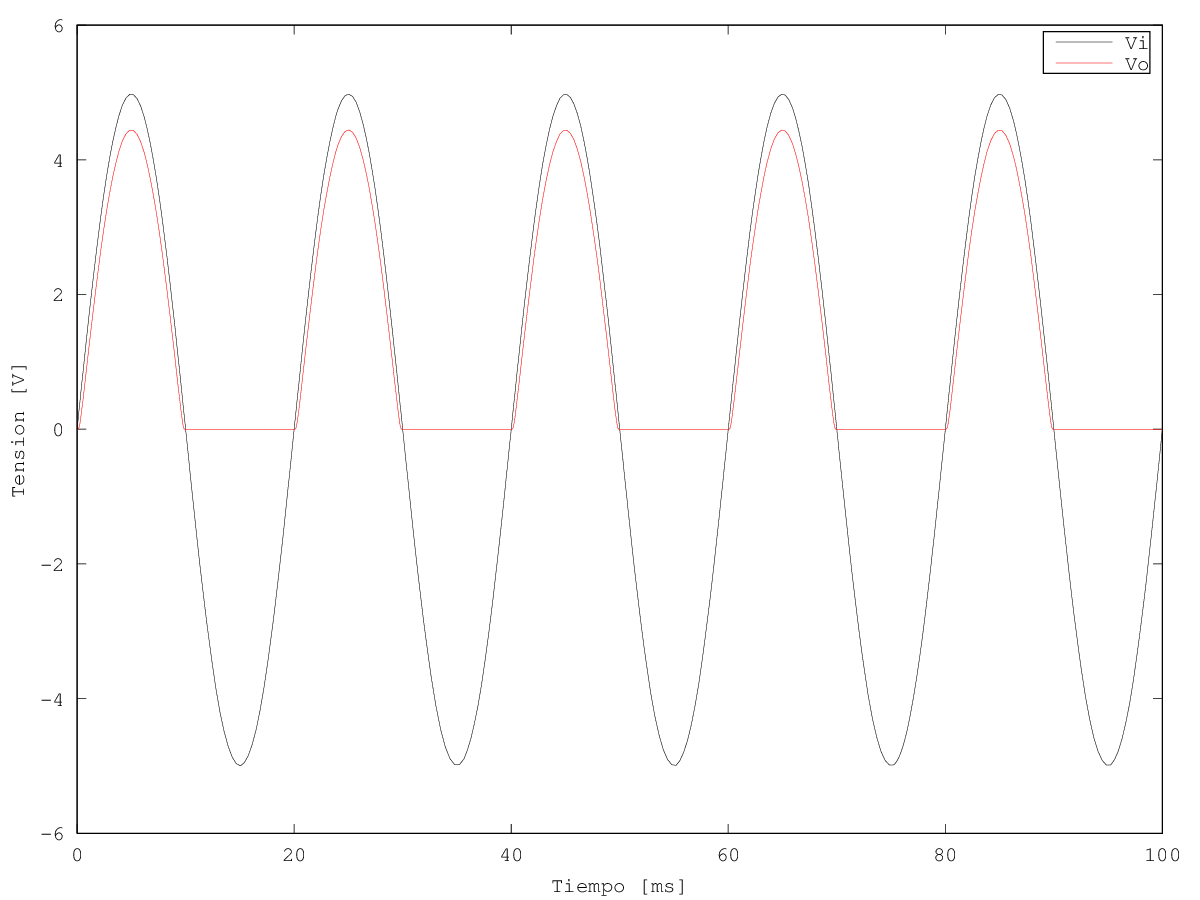
\includegraphics[width=0.8\textwidth]{gfxsantiago/FIG_SIM_Rectificador_Simple_3A1.png}
  \caption{Simulación de $v_{o}$ con señal de entrada de 50 Hz}
\end{figure}

\begin{figure}[H]
  \centering
      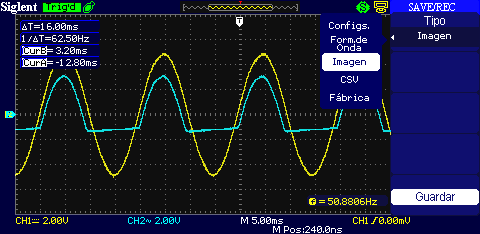
\includegraphics[width=0.8\textwidth]{gfxsantiago/FIG_MED_Rectificador_Simple_3A1.png}
  \caption{Medición de $v_{o}$ (azul) y $v_{i}$ (amarillo) con señal de entrada de 50 Hz}
\end{figure}

\noindent$\blacktriangle$\textbf{ ¿Por qué se utiliza una amplitud de 5 V en la excitación y no de 50 mV?}

La amplitud de la señal de excitación no puede ser de valores pequeños, como por ejemplo 50 mV, ya que en ese caso no se supera la tensión necesaria para que el diodo permita el paso de corriente.\\

A partir de las simulaciones realizadas se obtuvo un valor de 4,4 V pico para la tensión de salida $v_{o}$, cuyo valor medio (dado que se trata de una sinusoide rectificada) es $V_{o (medio)} = \hat{V}_{i}/\pi$ = 1,4 V.\\

\begin{figure}[H]
  \centering
      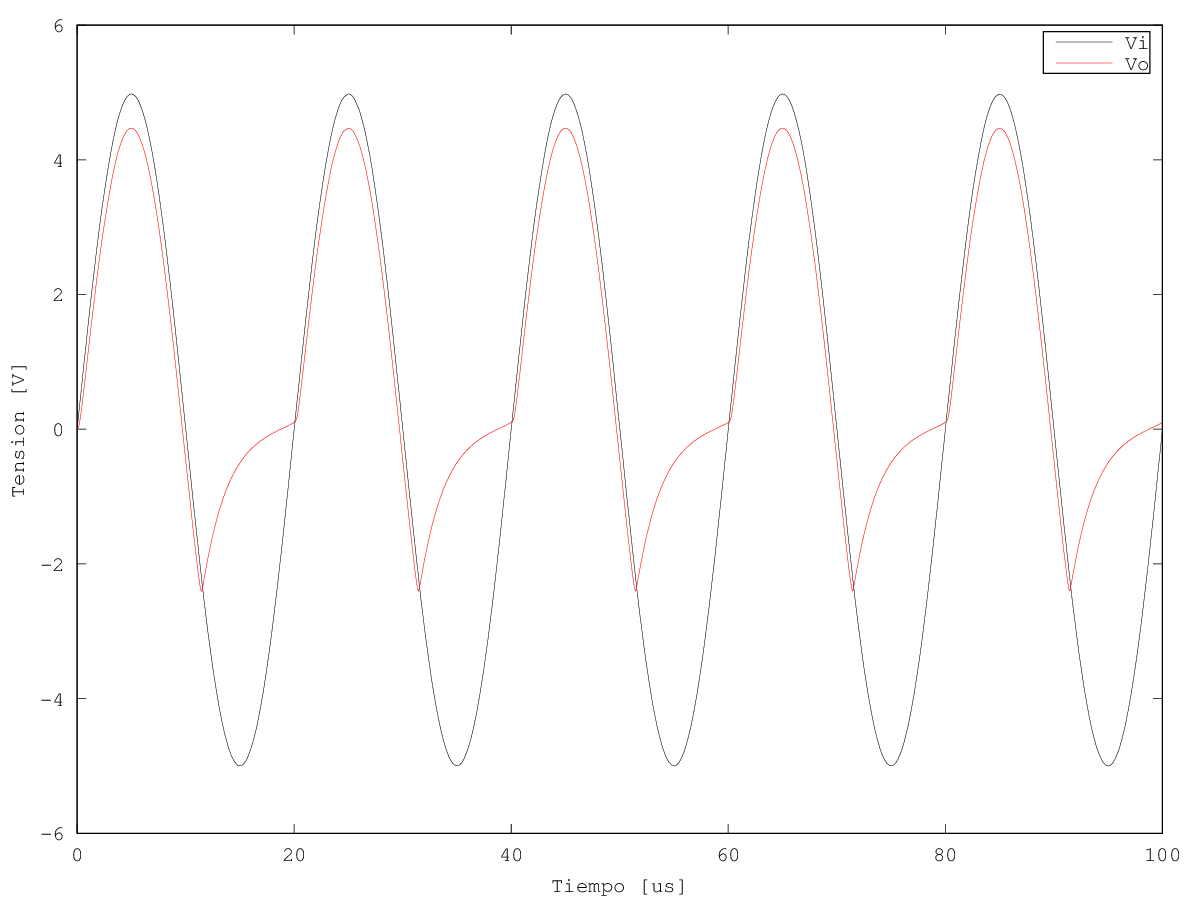
\includegraphics[width=0.8\textwidth]{gfxsantiago/FIG_SIM_Rectificador_Simple_3A2.png}
  \caption{Simulación de $v_{o}$ con señal de entrada de $50kHz$}
  \label{fig:sim_3A2}
\end{figure}

En estas mismas condiciones se incrementó la frecuencia de la señal de entrada a 50 kHz y la salida obtenida se puede observar en la Figura \ref{fig:sim_3A2}. En este caso, lo que sucede es que el tiempo de recuperación del diodo 1N4001 no permite la utilización de frecuencias tan altas, lo que tiene como consecuencia que no se puede utilizar el modelo de diodo al que estamos acostumbrados y eso se confirma al comparar las simulaciones para $v_{o}$ con $50Hz$ y $50kHz$.\\

Seguidamente se procede a conectar un capacitor de 47 $\mu F$ en paralelo a $R_{L}$, manteniendo el resto del banco de medición igual que antes (Figura \ref{fig:circ_3B}). Aquí, a partir de los datos obtenidos en las simulaciones y en las mediciones realizadas en el laboratorio es posible obtener valores de $v_{o (medio)}$, $v_{ripple}$ y el $z\%$ o porcentaje de ripple con la ayuda de las siguientes ecuaciones:

\begin{equation}
v_{ripple (ef)} = ( V_{o1 (ef)}^{2} + V_{o2 (ef)}^{2} + \ldots )^{1/2}
\end{equation}

\begin{equation}
z\% = 100 \frac{v_{ripple (ef)}}{v_{o (medio)}} 
\end{equation}

Para poder obtener los valores de $V_{oj (ef)}$, los cuales corresponden a las j-ésimas componentes de Fourier de la onda $V_{o}$ se hizo uso de la función FFT del LTSpice y del osciloscopio.\\

Los resultados se expresan a continuación en la Tabla \ref{table:rect_simple} y también se grafican las curvas correspondientes a $v_{o}$ para cada valor de $R_{L}$ en las Figuras \ref{fig:sim_3B1} a \ref{fig:med_3B3}. La presencia del capacitor genera que $v_{o}$ se mantenga dentro de un rango de valores denominado $v_{ripple}$ en vez de ser igual a la sinusoide rectificada como venia sucediendo. Si bien antes también podíamos considerar que había un capacitor en paralelo a la carga a partir del modelo de Thevenin de la punta 1x, este es de un valor muy pequeño como para que se acumule la carga necesaria para formar un ripple. Otra forma de ver esto último es a través de la constante de tiempo ($\tau$) del circuito que se forma, a partir del cual se puede aproximar el tiempo de carga y descarga del capacitor como:

\begin{equation}
5 \tau = 5 R C = 5 \cdot 10 k\Omega \cdot 200 pF = 10 \mu s
\end{equation}
mientras que al agregar el capacitor en paralelo, se modifica la constante de la siguiente manera: 

\begin{equation}
5 \tau = 5 R C = 5 \cdot 10 k\Omega \cdot 47\mu F = 2,35 s
\end{equation}

Además, al aumentar el valor de $R_{L}$ disminuye la corriente que puede circular por ella, con lo cual el capacitor se descarga más lentamente y $v_{ripple}$ disminuye.

Una de las observaciones que se pueden realizar sobre las gráficas realizadas es que al disminuir el valor de $R_{L}$, el semiciclo de la señal de entrada se deforma (esto es más claro en las figuras correspondientes a una carga de 1 $k\Omega$). Esto sucede porque el generador de funciones no es capaz de proveer la corriente que le esta demandando el circuito (la resistencia equivalente del generador tiene una caída de tensión interna) y solo tiene lugar en el semiciclo positivo ya que en el negativo el diodo no permite que circule corriente.

\begin{figure}[H]
  \centering
      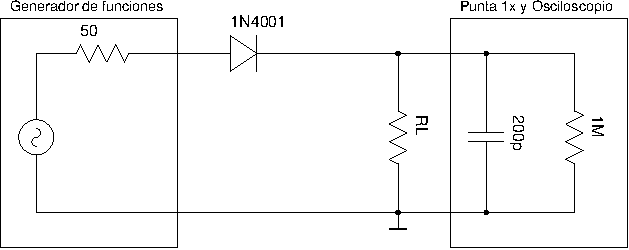
\includegraphics[width=0.8\textwidth]{gfxsantiago/FIG_CIRC_Rectificador_Simple_B.pdf}
  \caption{Circuito correspondiente al rectificador simple y capacitor junto con el banco de medición utilizado y los equivalentes Thevenin de los instrumentos que fueron considerados para las simulaciones.}
  \label{fig:circ_3B}
\end{figure}

\begin{figure}[H]
  \centering
      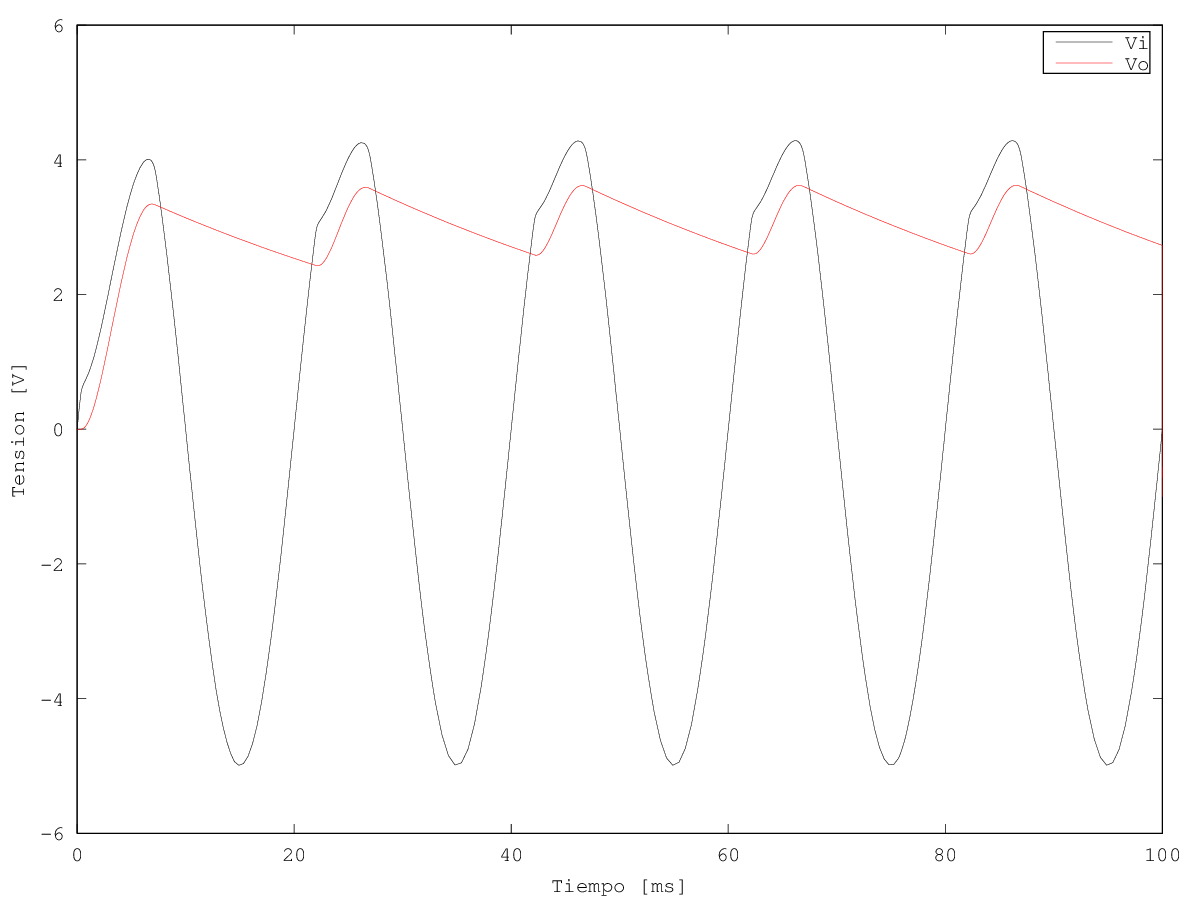
\includegraphics[width=0.8\textwidth]{gfxsantiago/FIG_SIM_Rectificador_Simple_3B1.png}
  \caption{Simulación de $v_{o}$ con $R_{L}$ = 1 $k\Omega$}
  \label{fig:sim_3B1}
\end{figure}

\begin{figure}[H]
  \centering
      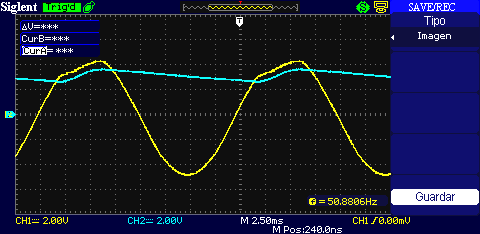
\includegraphics[width=0.8\textwidth]{gfxsantiago/FIG_MED_Rectificador_Simple_3B1.png}
  \caption{Medición de $v_{o}$ (azul) y $v_{i}$ (amarillo) con $R_{L}$ = 1 $k\Omega$}
\end{figure}

\begin{figure}[H]
  \centering
      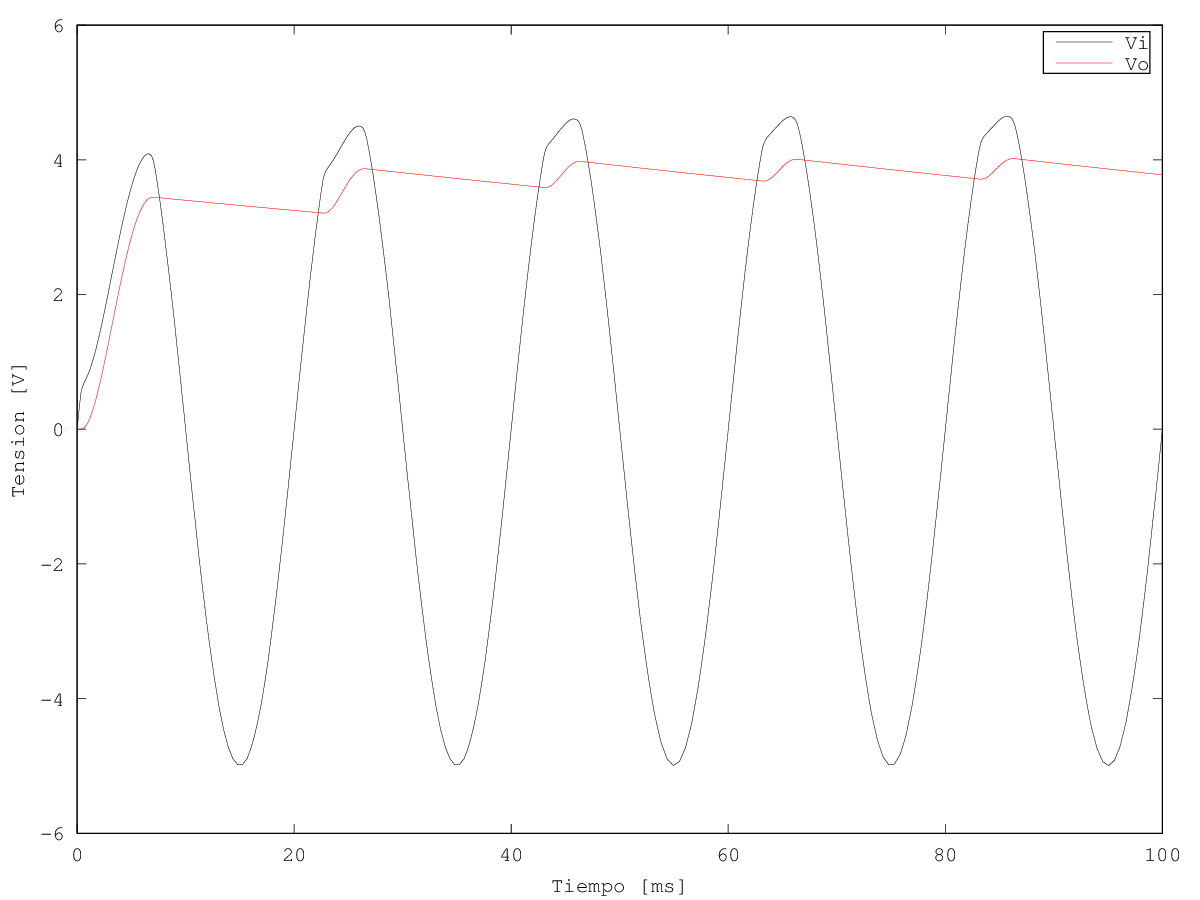
\includegraphics[width=0.8\textwidth]{gfxsantiago/FIG_SIM_Rectificador_Simple_3B2.png}
  \caption{Simulación de $v_{o}$ con $R_{L}$ = 4,7 $k\Omega$}
\end{figure}

\begin{figure}[H]
  \centering
      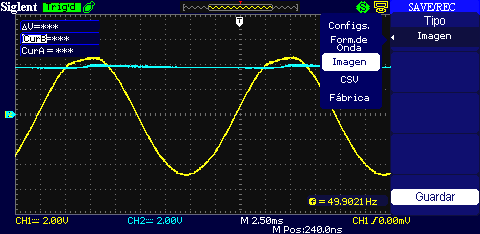
\includegraphics[width=0.8\textwidth]{gfxsantiago/FIG_MED_Rectificador_Simple_3B2.png}
  \caption{Medición de $v_{o}$ (azul) y $v_{i}$ (amarillo) con $R_{L}$ = 4,7 $k\Omega$}
\end{figure}

\begin{figure}[H]
  \centering
      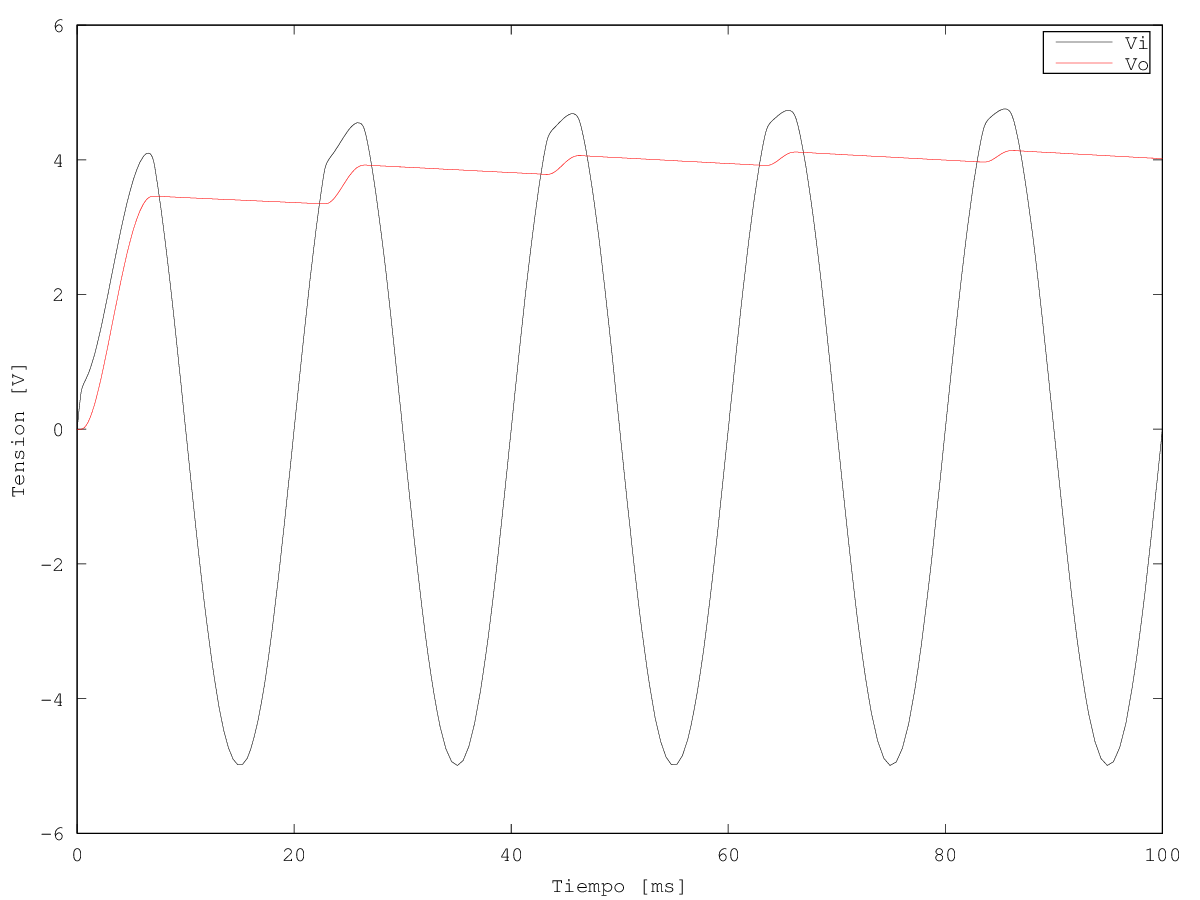
\includegraphics[width=0.8\textwidth]{gfxsantiago/FIG_SIM_Rectificador_Simple_3B3.png}
  \caption{Simulación de $v_{o}$ con $R_{L}$ = 10 $k\Omega$}
\end{figure}

\begin{figure}[H]
  \centering
      \includegraphics[width=0.8\textwidth]{gfxsantiago/FIG_MED_Rectificador_Simple_3B3.png}
  \caption{Medición de $v_{o}$ (azul) y $v_{i}$ (amarillo) con $R_{L}$ = 10 $k\Omega$}
  \label{fig:med_3B3}
\end{figure}

\begin{table}
\centering
\begin{tabular}{ccccccc}
\toprule
Carga $R_{L}$  & \multicolumn{3}{c}{Simulación}  & \multicolumn{3}{c}{Medición} \\

             & $v_{ripple(ef)}$    & $v_{o(medio)}$    &   $z\%$	& $v_{ripple(ef)}$    & $v_{o(medio)}$    &   $z\%$ \\
\midrule
1 $k\Omega$            & 0,33 V    & 3,68 V   & 9 \%	& 0,32 V    & 3,07 V   & 10\% \\
4,7 $k\Omega$            & 0,16 V    & 4,18 V   & 4 \%	& 0,08 V    & 3,83 V   & 2\% \\
10 $k\Omega$            & 0,1 V    & 4,28 V   & 2,5 \%	& 0,04 V    & 4,02 V   & 1\% \\
\bottomrule
\end{tabular}
\caption{}
\label{table:rect_simple}
\end{table}

\noindent$\blacktriangle$\textbf{ ¿Para qué sirve la curva llamada característica de regulación?}

A partir del análisis de la gráfica de dicha curva es posible analizar como varía la tensión media de salida del circuito según varía la carga $R_{L}$. Al aumentar la carga esto provoca una disminución de la corriente que circula por ella cuando el capacitor se esta descargando, con lo cual el ripple va haciéndose más pequeño (y $v_{o (medio)}$ aumenta).

\begin{figure}[H]
  \centering
      \includegraphics[width=0.8\textwidth]{gfxsantiago/FIG_Rectificador_Simple_Caracterisica_Regulacion.png}
  \caption{Curva característica de regulación obtenida en simulaciones y mediciones con osciloscopio.}
\end{figure}

\noindent$\blacktriangle$\textbf{ Proponer un banco de medición para medir la corriente a través del diodo. Justificar cualitativamente su forma y valores extremos.}

\begin{figure}[H]
  \centering
      \includegraphics[width=0.8\textwidth]{gfxsantiago/FIG_CIRC_Rectificador_Simple_Corriente_Diodo.pdf}
  \caption{Circuito propuesto para la medición de la corriente que circula por el diodo.}
  \label{circ:corr_diodo}
\end{figure}

Una posibilidad es colocar una resistencia pequeña (en este caso se eligió utilizar una de 50 $\Omega$) a la que llamaremos $R_t$ en serie entre el diodo y la carga, como muestra la figura \ref{circ:corr_diodo}. En estas condiciones se puede medir la tensión que cae sobre dicho resistor colocando dos puntas de medición entre sus terminales, obteniendo finalmente la corriente que circula por el diodo haciendo:

\begin{equation}
i_D = i_{R_t} = \frac{v_{t2} - v_{t1}}{R_t}
\end{equation}

En la figura \ref{fig:sim_corr_diodo} se muestran los resultados de la simulación realizada utilizando el circuito propuesto, el cual coincide con lo esperado ya que el diodo solo conduce cuando la señal de entrada esta en el semiciclo positivo, generando una corriente en el sentido propuesto en la figura \ref{circ:corr_diodo}.

\begin{figure}[H]
  \centering
      \includegraphics[width=0.8\textwidth]{gfxsantiago/FIG_SIM_Rectificador_Simple_Corriente_Diodo.png}
  \caption{Simulación de la corriente que circula por el diodo utilizando el método propuesto.}
  \label{fig:sim_corr_diodo}
\end{figure}

\noindent$\blacktriangle$\textbf{ Si en lugar de un rectificador de media onda se tuviese un puente rectificador de onda completa, ¿se esperaría un z\% mayor o menor?}

En el caso de un rectificador de onda completa, es fácil concluir que el porcentaje de rizado será menor que en el de media onda, ya que la tensión media de salida será mayor puesto que el tiempo durante el cual el capacitor se descarga es menor.\\


\subsection{Rectificador de media onda de precisión}
\begin{figure}[H]
  \centering
      \includegraphics[width=0.8\textwidth]{gfxsantiago/FIG_CIRC_Rectificador_Precision_B.pdf}
  \caption{Circuito correspondiente al rectificador de precisión junto con el banco de medición utilizado y los equivalentes Thevenin de los instrumentos que fueron considerados para las simulaciones.}
  \label{fig:circ_4A}
\end{figure}
En este caso se utilizará un circuito cuya principal diferencia con respecto al del punto 3.1 es la presencia de un amplificador operacional. El circuito correspondiente se puede observar en la Figura \ref{fig:circ_4A}. Las mediciones a realizar son bajo las mismas condiciones que las del punto 3.1.\\

\begin{figure}[H]
  \centering
      \includegraphics[width=0.8\textwidth]{gfxsantiago/FIG_SIM_Rectificador_Precision_4A1.png}
  \caption{Simulación de $v_{o}$ con señal de entrada de 50 Hz}
\end{figure}

\begin{figure}[H]
  \centering
      \includegraphics[width=0.8\textwidth]{gfxsantiago/FIG_MED_Rectificador_Precision_4A1.png}
  \caption{Medición de $v_{o}$ (Canal 2) y $v_{i}$ (Canal 1) con señal de entrada de $50Hz$}
\end{figure}

\begin{figure}[H]
  \centering
      \includegraphics[width=0.8\textwidth]{gfxsantiago/FIG_SIM_Rectificador_Precision_4A2.png}
  \caption{Simulación de $v_{o}$ con señal de entrada de $50kHz$}
\end{figure}
En principio se utilizó como señal de entrada una sinusoide de 5 V pico y $50Hz$, junto con una resistencia de carga de 10 $k\Omega$. Es inmediato que el circuito, tal y como describe su nombre, rectifica manteniendo el semieje positivo de la señal de entrada prácticamente igual, a diferencia del caso del rectificador de media onda simple, en el cual había una diferencia entre $v_{o}$ y $v_{i}$ provocada por una caída de tensión en el diodo. Posteriormente se realizó la simulación correspondiente al mismo banco de trabajo pero modificando la frecuencia a $50kHz$. Las diferencias que se obtienen al realizar las simulaciones según se modifica la frecuencia de trabajo son notables y tiene la misma explicación que en el punto 3.1 para el diodo, a lo que hay que sumarle las variaciones respecto al modelo ideal de amplificador operacional según se aumenta la frecuencia, tal y como expresa la hoja de datos del AO LM741 (entre las cuales se destacan el aumento de la resistencia de salida, la disminución de la resistencia de entrada, etc.).

El funcionamiento del rectificador de precisión se puede subdividir según el semiciclo de la señal de entrada:
\begin{itemize}
  \item Semiciclo positivo: Viendo únicamente a las resistencias y considerando al amplificador como ideal es fácil concluir que $v_{o}$ será igual a $v_{i}$ pero de signo opuesto ya que la corriente que circula por ellas es la misma y son de igual valor (10 $k\Omega$). En este caso el diodo conectado entre la salida del operacional y $v_{o}$ conduce y genera una tensión de $v_{o} - 0,7 V$ en la salida del amplificador operacional, pero el diodo restante no permite que circule corriente puesto que no se cumple que $V_{D} < 0,7 V$, considerando a $V_{D}$ como la tensión entre el ánodo y cátodo del diodo.
  \item Semiciclo negativo: En este caso la corriente que circula por $R_{1}$ va en sentido contrario al de antes, por lo que el diodo que se encuentra entre la salida del operacional y el terminal de entrada negativo conduce esta corriente que esta provista por el AO. Dado que consideramos al operacional como ideal en ambos terminales de entrada hay una tierra virtual y como no circula corriente por $R_{2}$ se puede concluir que no cae tensión sobre ella y por lo tanto $v_{o} = 0 V$.
\end{itemize}

Luego, se procedió a colocar un capacitor de 47 $\mu F$ en paralelo a $R_{L}$, cuyo valor se fue aumentando al igual que en el punto anterior, es decir, 1 $k\Omega$, 4,7 $k\Omega$ y 10 $k\Omega$. Para estos tres casos se simuló y se midió con la ayuda de un osciloscopio el valor de $v_{o}$ y los resultados están expresados en las Figuras \ref{fig:sim_4B1} a \ref{fig:med_4B3}. Al igual que antes la presencia del capacitor genera que la tensión $v_{o}$ se mantenga dentro de un rango de valores reducido llamado $v_{ripple}$, y a medida que aumenta el valor de la resistencia $R_{L}$ el ripple va disminuyendo. Los resultados obtenidos para $v_{ripple(ef)}$, $v_{o(medio)}$ y $z\%$ correspondientes tanto a las simulaciones como a las mediciones se pueden observar en la tabla \ref{table:rect_precision}. \\

\begin{table}
\centering
\begin{tabular}{ccccccc}
\toprule
Carga $R_{L}$  & \multicolumn{3}{c}{Simulación}  & \multicolumn{3}{c}{Medición} \\

             & $v_{ripple(ef)}$    & $v_{o(medio)}$    &   $z\%$	& $v_{ripple(ef)}$    & $v_{o(medio)}$    &   $z\%$ \\
\midrule
1 $k\Omega$            & 0,3 V    & 4,15 V   & 7 \%	& 0,48 V    & 7,34 V   & 6\% \\
4,7 $k\Omega$            & 0,2 V    & 4,72 V   & 4 \%	& 0,16 V    & 8,40 V   & 2\% \\
10 $k\Omega$            & 0,17 V    & 4,8 V   & 3,5 \%	& 0,12 V    & 8,63 V   & 1\% \\
\bottomrule
\end{tabular}
\caption{}
\label{table:rect_precision}
\end{table}

\begin{figure}[H]
  \centering
      \includegraphics[width=0.8\textwidth]{gfxsantiago/FIG_SIM_Rectificador_Precision_4B1.png}
  \caption{Simulación de $v_{o}$ con $R_{L}$ = 1 $k\Omega$}
  \label{fig:sim_4B1}
\end{figure}

\begin{figure}[H]
  \centering
      \includegraphics[width=0.8\textwidth]{gfxsantiago/FIG_MED_Rectificador_Precision_4B1.png}
  \caption{Medición de $v_{o}$ (Canal 2) y $v_{i}$ (Canal 1) con $R_{L}$ = 1 $k\Omega$}
\end{figure}

\begin{figure}[H]
  \centering
      \includegraphics[width=0.8\textwidth]{gfxsantiago/FIG_SIM_Rectificador_Precision_4B2.png}
  \caption{Simulación de $v_{o}$ con $R_{L}$ = 4,7 $k\Omega$}
\end{figure}

\begin{figure}[H]
  \centering
      \includegraphics[width=0.8\textwidth]{gfxsantiago/FIG_MED_Rectificador_Precision_4B2.png}
  \caption{Medición de $v_{o}$ (Canal 2) y $v_{i}$ (Canal 1) con $R_{L}$ = 4,7 $k\Omega$}
\end{figure}

\begin{figure}[H]
  \centering
      \includegraphics[width=0.8\textwidth]{gfxsantiago/FIG_SIM_Rectificador_Precision_4B3.png}
  \caption{Simulación de $v_{o}$ con $R_{L}$ = 10 $k\Omega$}
\end{figure}

\begin{figure}[H]
  \centering
      \includegraphics[width=0.8\textwidth]{gfxsantiago/FIG_MED_Rectificador_Precision_4B3.png}
  \caption{Medición de $v_{o}$ (Canal 2) y $v_{i}$ (Canal 1) con $R_{L}$ = 10 $k\Omega$}
  \label{fig:med_4B3}
\end{figure}

\begin{figure}[H]
  \centering
      \includegraphics[width=0.8\textwidth]{gfxsantiago/FIG_Rectificador_Precision_Caracterisica_Regulacion.png}
  \caption{Curva característica de regulación obtenida en simulaciones y mediciones con osciloscopio.}
\end{figure}

\noindent$\blacktriangle$\textbf{ ¿Qué sucede si se reemplaza $R_2$ = 10 $k\Omega$ por un resistor de 22 $k\Omega$?}

En estas condiciones, a partir del análisis del circuito se puede predecir que el valor pico de $v_{o}$ aumentará prácticamente el doble. Esto se verifica tanto en las simulaciones (Figura \ref{fig:sim_4C}) y en las mediciones (Figura \ref{fig:med_4C}) pero también se observa que la señal tiene distorsión en los picos . Esto sucede debido a que en esos casos la tensión de salida es superior a lo que puede proveer el operacional.\\

\begin{figure}[H]
  \centering
      \includegraphics[width=0.8\textwidth]{gfxsantiago/FIG_SIM_Rectificador_Precision_4C.png}
  \caption{Simulación de $v_{o}$ con $R_{2}$ = 22 $k\Omega$}
  \label{fig:sim_4C}
\end{figure}

\begin{figure}[H]
  \centering
      \includegraphics[width=0.8\textwidth]{gfxsantiago/FIG_MED_Rectificador_Precision_4C.png}
  \caption{Medición de $v_{o}$ (Canal 2) y $v_{i}$ (Canal 1) con $R_{2}$ = 22 $k\Omega$}
  \label{fig:med_4C}
\end{figure}

\noindent$\blacktriangle$\textbf{ ¿Qué sucede si se invierte la conexión de cada diodo?}

La inversión de las conexiones de cada diodo del circuito tendrá como consecuencia que cuando la señal de entrada se encuentra en su semiciclo positivo se tendrá 0 V en la salida mientras que cuando $v_{i}$ esta en el semiciclo negativo $v_{o}$ valdrá igual pero con signo opuesto. En la figura \ref{fig:sim_4D} se puede ver la gráfica de los datos obtenidos al simular esta situación, corroborando el análisis realizado.

\begin{figure}[H]
  \centering
      \includegraphics[width=0.8\textwidth]{gfxsantiago/FIG_SIM_Rectificador_Precision_4D.png}
  \caption{Simulación de $v_{o}$ con diodos invertidos}
  \label{fig:sim_4D}
\end{figure}

\clearpage
\section{Conclusiones}
\label{sec:conclu}

Durante el desarrollo de este trabajo se fueron verificando las hipótesis con las que se partió: los modelos ideales son aplicables solamente en determinadas situaciones. En el caso de no tener en cuenta estas condiciones se pueden encontrar con resultados imprevistos a la hora de trabajar con circuitos cuyo correcto funcionamiento solo puede ser predicho si se trabaja con una modelización apropiada.

En principio, bajo las condiciones que se analizaron, se encontró que el amplificador operacional tiene un ancho de banda limitado, esto implica que su impedancia de salida no es cero. También, en la experiencia en la que se trabajó con resistencias del orden de $1M\Omega$, se corroboró que la impedancia de entrada no es infinito. A su vez, su salida no puede superar la tensión de alimentación, lo que produce las alinealidades y los recortes ya vistos.

En el caso de los circuitos rectificadores ésto se evidenció principalmente a la hora de intentar aplicar al diodo señales de alta frecuencia para las cuales no fue diseñado, lo que introdujo un efecto capacitivo al sistema.

Por otro lado, en algunos ejercicios también fue necesario considerar los modelos no ideales de los instrumentos para que la respuesta de la simulación sea semejante a la medición. Esto sucedió en la deformación de la señal generada en el rectificador.

% Habías escrito algo del ancho de banda del operacional antes, lo corregí porque el BW del opamp es de 1MHz, y eso no lo probamos.


\cleardoublepage
% --------------------------------------------------
% BIBLIOGRAFÍA
%\bibliography{biblio}{}
%\bibliographystyle{plain}
%\clearpage
% --------------------------------------------------
\end{document}